\documentclass[binding=0.6cm, LaM]{sapthesis}
\usepackage{microtype}
\usepackage[english]{babel}
\usepackage[utf8]{inputenx}
\usepackage{hyperref}
\usepackage{wasysym}
\usepackage{siunitx}
\usepackage{titlesec}
\usepackage{float}
\usepackage{xcolor}
\usepackage{nameref}
\usepackage{verbatim}
\usepackage{natbib}
\newcommand{\fpg}[1]{\textcolor{red}{#1} }
\newcommand\apjl{The Astrophysical Journal Letters}
\newcommand\apj{The Astrophysical Journal}
\newcommand\prl{Physical Review Letters}
\newcommand\mnras{Monthly Notices of the Royal Astronomical Society}
\newcommand\prd{Physical Review D}
\newcommand\nat{Nature}
\newcommand\physrep{Physics Reports}
\DeclareUnicodeCharacter{2009}{\,} 
\hypersetup{pdftitle={My thesis},pdfauthor={Giada Caneva Santoro}}
\usepackage{amsmath, amssymb}
\title{Coherent and Coincident Analyses of LIGO-Virgo Data from the Third Observing Run}
\author{Giada Caneva Santoro}
\IDnumber{1490713}
\course{Facolt\`a di Scienze Matematiche Fisiche e Naturali}
\courseorganizer{Corso di Laurea Magistrale in Fisica}
\AcademicYear{2018/2019}
\copyyear{2020}
\advisor{Dr. Francesco Pannarale Greco}
\authoremail{giada.greenday92@gmail.com}
\DeclareUnicodeCharacter{2212}{-}

\usepackage{natbib}
\begin{document}

\frontmatter
\maketitle
\dedication{Se non tengo presente l’universo, perdo il senso delle proporzioni. \\ Italo Calvino.}


\tableofcontents

\begin{acknowledgments}
We are grateful for computational resources provided by Cardiff University, and funded by an STFC grant supporting UK Involvement in the Operation of Advanced LIGO.
\end{acknowledgments}

\mainmatter 

\chapter*{Introduction}
\label{sec:intro}
\addcontentsline{toc}{chapter}{Introduction}
\markboth{Introduction}{Introduction}
%
\fpg{In vari punti usi {\ttfamily cite\{\}}. Inoltre citi senza averle in biblio 213 e 215.  Nella bibliografia hai varie entries solo come arXiv preprints, anche per roba gi\`a pubblicata!}%
\fpg{Giri di correzione: 1.}%
	More than 100 years ago, Albert Einstein predicted the existence of gravitational waves (GWs) starting from his theory of general relativity \cite{1,2}.
	He discovered that the acceleration of masses
	can cause distortions in the curvature of spacetime that 
        spread throughout spacetime itself at the speed of light, similarly to the ripples in a pond when a stone is tossed in it.
	He derived that the amplitude of GWs would be extremely small and concluded that it would be impossible to detect them with any of the technology foreseen at his time.

	Nowadays, roughly a century later, we are able to directly detect GWs.  
	The most energetic GWs are generated when high speeds and compact objects, that is, 	
	celestial bodies with a high concentration of gravitational mass per unit volume, are involved.
	Orbiting pairs of black holes (BHs) and neutron stars (NS), the densest objects in the universe,
	are therefore efficient GW emitters and are indeed present in all the GW sources detected by the LIGO-Virgo Collaboration so far.
        BHs and NSs result from the gravitational collapse of massive progenitor stars.
        BHs represent the extremes of spacetime curvature:
        they contain a singularity, have no surface, and possess an event horizon that separates the information
        from within the BH interior from the rest of the universe.
        They are extraordinary cosmic laboratories to probe gravity in the strong-field regime.
        Astrophysical BHs are entirely described by two parameters: their gravitational mass and their rotational angular momentum (spin).
        On the other hand, NSs are extreme objects from the point of view of all fundamental forces, 
	as their masses fall in the range $1$--$2.5M_\odot$, while their radii are of the order of 10\,km; 
	additionally, they are equipped with magnetic fields that can exceed $10^{15}\,$G 
	(in this case one refers to the NS as magnetar). 
	One of the main difficulties in modelling NSs is that the equation of state that governs the microphysics in their interiors is currently unknown.

        Binaries of NSs and BHs are collectively called compact binaries,
        and come in three flavours: systems that consist of two NSs (indicated as BNSs, for binary NSs), 
	of two BHs (indicated as BBHs, for binary BHs), or of a BH and an NS (indicated as NSBHs).
        As the two compact objects orbit one another, the binary loses orbital energy and orbital angular momentum, 
	as both are radiated away via GWs.
        As a results, the two compact objects spiral in towards each other, 
	reaching extreme velocities ($\sim 0.5c$) at the very end of this process. 
        At the end of the inspiral, the two compact companions merge and 
	the GW emission reaches its peak. 
	The newly formed remnant then settles down emitting a weak GW signal that dies out.  
	This whole process goes under the name of compact binary coalescence (CBC).
	In the final fraction of a CBC, a significant amount of gravitational mass is converted 
	into gravitational energy carried away by the GWs.  
	These waves fall within the frequency range of current terrestrial GW detector, 
	if the binary contains NSs and/or BHs with masses up to $\mathcal{O}(100M_\odot)$.
        The masses of the objects involved dictate the how long the GW signal they emit 
	lasts in the $\sim 10$--$1000$\,Hz sensitivity band of current detectors.
        More massive binaries merge at lower frequencies and therefore have fewer cycles in band.
        For example, the first GW signal ever detected, GW150914, came from the coalescence of two fairly massive BHs: 
	the signal was visible for only two-tenths of a second \cite{14}, as discussed in Sec.\,\ref{subsec:GW150914}. 
        BNS systems, by contrast, accumulate many cycles in the instrumental band.
        The first BNS coalescence witnessed by LIGO-Virgo, GW170817, 
	generated a GW signal that lasted $\sim 100\,$s in the sensitivity window of the detectors \cite{15}, 
	as described in Sec.\,\ref{subsec:GW170817}.
	The observation of GW150914 (Sec.\,\ref{subsec:GW150914}) was a truly remarkable accomplishment: 
	it \emph{directly}\footnote{Until then, GWs had only been observed indirectly by using pulsar timing to monitor 
        their effect on the orbit of pulsar binary star systems.} confirmed Einstein's prediction of the existence of GWs, 
	and it demonstrated that stellar-mass BBH systems form in the universe and merge within a Hubble time.
	This event marked the beginning of a new era of GW astronomy, 
	which enables the observations of violent astrophysical events that are not visible with traditional astronomy.
	The BNS merger GW170817 (Sec.\,\ref{subsec:GW170817}) marked, instead, the beginning of multi-messenger astronomy 
	because as it was the first GW observation with recorded electromagnetic counterparts.  	

	The LIGO-Virgo GW network routinely performs multiples searches aimed at detecting signals 
	emitted by all three kinds of CBCs\footnote{See Sec.\,\ref{sec:sources} for a brief overview of other kinds of searches.}.
        These are run both online, to detect and report compact binary merger events 
	with sub-minute latencies, and offline, to take advantage of improved data calibration 	
	and of additional information regarding data quality to produce a more sensitive search.
	This thesis focuses on two kinds of offline analyses of a part of LIGO-Virgo data collected during the third observing run (O3).
        Specifically, I used the CBC matched-filtering search pipeline {\ttfamily PyCBC}, discussed in Chapter \ref{ch:datatools}, 
	to perform an all-sky search for BNS, NSBH, and BBH signals; further, I used the {\ttfamily PyGRB} pipeline, 
	discussed in Chapter \ref{ch:datanalysis}, to search for BNS and NSBH signals compatible 
	with the sky-location and time of three short gamma-ray bursts (GRBs) that occurred during O3.

	GRBs are short ($\Delta t \sim 0.1-100s$) and intense bursts of 
	electromagnetic radiation in the high-energy (1\,keV--10\,MeV) $\gamma$-ray spectrum.
	This radiation is produced when an ultra-relativistic fireball of high energy photons 
	is launched from a central engine, and it can be accompanied by a detectable afterglow emission 
	in the X-ray and sometimes optical and radio bands, as the fireball expands and cools down \cite{139}.
	GRBs can be broadly classified based on the timescale during which 5\% to 95\% of the counts are recorded ($T_{90}$)
	as either long GRBs, $T_{90} > 2\,$s or short GRBs, $T_{90} \leq 2\,$s.\footnote{For the purposes of the {\ttfamily PyGRB} analysis, the classification is augmented by factoring in the duration error $\delta T_{90}$: 
        when $T_{90}-|\delta T_{90}| > 4\,$s the GRBs are labelled as {\it long},
	when $T_{90}+|\delta T_{90}| \leq 2\,$s as {\it short},
        while the rest are labelled as {\it ambiguous}.  The purpose of this is to ensure that indeed {\it all} GRBs potentially generated by an NS binary coalescence --- i.e., short and ambiguous ones --- are followed up.}
	The two groups also show other differences.  
	Short GRBs have fainter afterglows and harder emission spectra than long GRBs; 
	they are also seen to have an offset relative to their host galaxy center \cite{154}.
	For decades, the exact origin of short GRBs was an open question in high-energy astrophysics.  
	The data indicated a compact source smaller than a stellar-scale object, 
	and a progenitor involving old astrophysical objects with a significant velocity with respect to the host galaxy.  
	BNS and NSBH mergers were the natural candidates as short GRB progenitors, 
	but the observational confirmation of this conjecture came with GW170817.
	This event marked the first direct observation of a BNS unambiguously associate to a short GRB, 
	GRB 170817 which followed $1.74\,$s after the GW trigger and was detected by {\it Fermi}/GBM and INTEGRAL SPI-ACS \cite{15}.
	The unambiguous association also allowed for the most precise comparison to date
	between the speed of GWs and the speed of light.  
	Further, it posed new constraints on alternative theories of gravity. 
	Subsequent electromagnetic follow-up of GW170817 showed that BNS merger events 
	help explain the origin of heavy elements in the universe.

	There remain several open questions surrounding these extreme and energetic events, 
	and multi-messenger astronomy with GWs has proven to be a resourceful means of gaining 
	knowledge of the astrophysical sources and their emission engines, 
	providing insight that electromagnetic observations alone cannot achieve.
	To mention a few examples of open problems, we do not yet know whether NSBH systems are also short GRB progenitors.  
	Similarly, the exact mechanism that launches the jet is currently not yet understood.
        These and other questions motivate the targeted searches for GWs at the sky-position and time of GRBs, 
	as they increase the chances of achieving joint GW-GRB detections.
	Knowing the time and sky-location of a sought for GW event
	allows to perform a deeper search in the GW data, potentially uncovering signals 
	that are not accessible to all-sky, all-time searches, as discussed in Chapter \ref{subsec:coincident}.

	Since the observed properties of short GRBs may be attributed to matter accretion onto a BH,
	following the tidal disruption of a NS, in addition to BNSs, NSBH systems are also considered likely short GRBs progenitors.
	At the time of writing this work, no certain NSBH coalescence has been observed.
	This motivates further the use of 
	offline GW searches targeting short GRB triggers, as the one I conducted in Chapter \ref{ch:datanalysis}.
	To enable this search in O3, I also generated and validate the set of waveforms used to filter the data (see discussion in Sec\,\ref{subsec:construction_and_validation})
	This specific set of waveform is known as an ``EM-bright template bank,'' 
	as it covers only BNSs and NSBH systems that have undergone tidal disruption and are thus potential short GRB progenitors.

	This thesis is organized as follows: Chapter \ref{ch:GWDetectionPrinciples} provides a theoretical introduction to gravitational waves and 
	describes the LIGO and Virgo detectors and the physics behind its purpose, and noise sources.
	Chapter \ref{ch:datatools} gives an introduction to data analysis tools for a matched filtering source, 
	describes the generation of template banks and signal consistency tests.
	It then provides an overview of coherent vs coincident searches; the last section describes injections.
	Chapter \ref{ch:ObservingRuns} gives a summary of the gravitational wave detection from the first to the third observing run.
	Chapter \ref{ch:datanalysis} illustrates the difference between the old and new model for the remnant mass of a neutron star-black hole system.
	It then describes how the template bank has been updated and how well it works.
	Finally, the results of the offline {\ttfamily PyCBC} and {\ttfamily PyGRB} search are presented and discussed.

%----------------------------------------------------------------------------------------------------------------------------------------------------------------------------------------------------------
\chapter{Gravitational-Wave Detection Principles}
\label{ch:GWDetectionPrinciples}
\fpg{Giri di correzione: 1.}%
	The aim of this thesis is to expose the methodologies involved 
	in compact binary coalescence through gravitational wave observation. 
	Before giving into this topic, it is useful to shortly discuss gravitational waves, 
	the theory behind them and the instrumental apparatus that is being used to detect them. 
	In this chapter we give a broad outline of these subjects, 
	without going too deep into details.

	We begin by introducing the basics of gravitational wave theory in section 2.1. 
	In section 2.2 we discuss gravitational wave interferometric detectors. 
	In section 2.3 we briefly describe the noise sources that affect the detection. 
	Finally. in section 2.4, we describe the astrophysical sources of gravitational radiation.

\section{Gravitational Waves in Linearized Gravity}

	In 1915, Albert Einstein presented his general theory of relativity
	The classical Newtonian notion of gravity, which stated that gravity arises from an 
	action at a distance, was replaced by a geometric interpretation of the Universe, 
	the spacetime continuum: this may be regarded as a fabric and that can be curved 
	by mass \cite{1}. 
	The motion of masses on this curved spacetime fabric will then be perceived as gravity. 
	In general relativity, spacetime is regarded as a four-dimensional manifold 
	with a Lorentzian metric, and gravity is a manifestation of the manifold’s curvature.

	The space-time curvature is associated with the stress-energy tensor 
	of matter fields through the Einstein field equation:
		\begin{equation}
		G_{\mu\nu} \equiv R_{\mu\nu}  - {\frac{1}{2}}g_{\mu\nu}R = \frac{8\pi G_{N}}{c^4}T_{\mu\nu} 
		\end{equation}
	where $G_{\mu\nu} $ is the Einstein tensor, $T_{\mu\nu} $ is the stress-energy 
	tensor of matter-fields, $ G_{N}$ is Newton’s gravitational constant and $c$ the speed of light.

	In 1916 Einstein found the weak-field solutions to general relativity had wave-like solutions, GWs.
	GWs are ripples in the fabric of spacetime, 
	which periodically lengthen and shorten space, and speed up and slow down time \cite{2}.
 	To study the properties of GWs, it is instructive to first study them 
	in situations where the gravitational fields are weak.
	In the so-called weak-field approximation, one can view the metric as the Minkowski metric 
	with a small perturbation: the Einstein equations can be expanded around the flat-space metric, of special relativity.

	Letting $ x_\mu = (t, x, y, z)$ denote the time and space coordinates, 
	we can write the proper distance between events $x_{\mu}$ and $x_{\mu} + dx_{\mu}$ as
		\[
		ds^2 = g_{\mu\nu}dx^{\mu}dx^{\nu} \approx (\eta_{\mu\nu} + h_{\mu\nu})dx_{\mu}dx_{\nu}. \hspace*{2cm}\|h_{\mu\nu}\|\ll 1
		\]
	Here $\eta_{\mu\nu} = diag(-1,1,1,1)$ is the usual Minkowski metric and the metric perturbation  $h_{\mu\nu}$        
	represents the linearised gravitational field, it encapsulates GWs, 
	but contains additional, non-radiative degrees of freedom as well. $\|h_{\mu\nu}\|$ means
	“the magnitude of a typical non-zero component of $h_{\mu\nu}$”. 
	The condition $\|h_{\mu\nu}\|\ll 1$ requires both the gravitational field to be weak, 
	and constrains the coordinate system to be approximately Cartesian.

	In linearized gravity, the smallness of the perturbation means that only terms which are linear in $h_{\mu\nu}$ are considered;
	higher order terms are discarded. As a consequence, indices are raised and lowered using the flat metric. 
	The metric perturbation $h_{\mu\nu}$ transforms as a tensor under Lorentz transformations, 
	but not under general coordinate transformations: since the numerical values of the components
	of a tensor depend on the reference frame, there exists a reference frame in which 
	the linearisation of the gravitational field holds on a sufficiently large region of the spacetime.
        
	The Einstein field equations are covariant under general coordinate transformations
		\begin{equation}
		x^{\mu} \rightarrow x^{\mu ‘}(x)
		\end{equation}
	So that the metric transforms as
		\begin{equation}
		g_{\mu\nu} \rightarrow g_{\mu^\prime\nu^\prime} = x^{\rho},_{\mu^\prime}x^{\sigma},_{\nu^\prime}g_{\rho \sigma}
		\end{equation}
	This means that one is free to choose a convenient coordinate system without 
	altering the physical predictions of the field equations \cite{16}.

	Choosing a reference frame breaks the invariance of general relativity under 
	coordinate transformations but it also erases spurious degrees of freedom. 
	After choosing a frame where the field is linearised, 
	a residual gauge symmetry remains.

	Under infinitesimal coordinate transformations
                 \[
			x_{\mu} \rightarrow x_{\mu} + \xi_{\mu}
                \]
	using the transformation law of the metric, to lowest order $h_{\mu\nu}$ transforms as	
		\[
			h_{\mu\nu} \rightarrow h_{\mu\nu} - \partial_{\mu}\xi_{\nu} - \partial_{\nu}\xi_{\mu}
		\]
	Rather than working with the metric perturbation, changing notation and using the trace-reversed perturbation 
	makes the computation more compact and cleaner. We define
		\begin{equation}
			{\bar h}_{\mu\nu} = h_{\mu\nu} - \frac{1}{2}\eta_{\mu\nu}h  
		\end{equation}
	the trace
		\begin{equation}
			h = \eta^{\mu\nu}h_{\mu\nu}
		\end{equation}
	and express the trace-reversed field:
		\begin{equation}
			h_{\mu\nu} = {\bar h}_{\mu\nu} + \frac{1}{2}\eta_{\mu\nu}{\bar h}
		\end{equation}
	The Rienmann tensor constructed in the linearised theory is given by
		\begin{align}
			R^{\mu}_{\nu\rho\sigma} &= \partial_{\rho} \Gamma^{\mu}_{\nu\sigma} - \partial_{\sigma}\Gamma^{\mu}_{\nu\rho}  \\
				       &= \frac{1}{2} (\partial_{\rho}\partial_{\nu}h^{\mu}_{\nu\rho} + \partial_{\sigma}\partial^{\mu}h^{\nu\rho} - \partial_{\rho}\partial^{\mu}h^{\nu\sigma} - \partial_{\					     \sigma}\partial_{\nu}h^{\mu}_{\rho})
		\end{align}
	From this, the Ricci tensor takes the form
		\begin{equation}
			R_{\mu\nu} = R^{\rho}_{\mu\rho\nu} = \frac{1}{2}(\partial_{\rho}\partial_{\nu}h^{\rho}_{\mu} + \partial^{\rho}\partial_{\mu}h_{\nu\rho} - \square h_{\mu\nu} - \partial_{\mu}\partial_{\nu}h)
		\end{equation}
	The curvature scalar is obtained contracting once more:
		\begin{equation}
			R = R^{\mu}_{\mu} = (\partial_{\rho}\partial^{\mu}h^{\rho}_{\mu} - \square h)
		\end{equation}
	Finally, the Einstein tensor can be expressed as
		\begin{equation}
			G_{\mu\nu} = \frac{1}{2}(\partial_{\rho}\partial_{\nu}h^{\rho}_{\mu} + \partial^{\rho}\partial_{\mu}h_{\nu\rho} - \square h_{\mu\nu} - \partial_{\mu}\partial_{\nu}h - \eta_{\mu\nu}\partial_{\rho}\partial^{\sigma}h^{\rho}_{\sigma} + \eta_{\mu\nu}\square h)
		\end{equation}
	Substituting the metric perturbation $h_{\mu\nu}$  with the $trace-reversed$ perturbation ${\bar h}_{\mu\nu}$ and expanding, 
	the linearized Einstein equations take the compact form:
		\begin{equation}
			\square {\bar h}_{\mu\nu} + \eta_{\mu\nu}{\partial}^{\rho}{\partial}^{\sigma}{\bar h}_{\rho\sigma} - {\partial}^{\rho}{\partial}^{\nu}{\bar h}_{\mu\rho} - {\partial}^{\rho}{\partial}^{\mu}{\bar h}_{\nu\rho} = - \frac{16\pi G_{N}}{c^4}T_{\mu\nu}.
		\end{equation}
	The linearised equations of motion are gauge-invariant, and the gauge freedom can
 	be used to simplify the form of the field equations \cite{17}.
 	In the Lorentz family of gauges, choosing the harmonic gauge $ \partial_{\mu}h_{\mu\nu} = 0 $ 
	reduces the Einstein equations to a simple wave equation that relates the trace-reversed field
 	to the stress energy tensor:
		\begin{equation}
			\label{reduceinstein}
			\square {\bar h}_{\mu\nu} =({\partial^2 \over {\partial t^2} } - {\partial^2 \over {\partial x^2}}  - {\partial^2 \over {\partial y^2}}  -  {\partial^2 \over {\partial z^2}}) {\bar h}_{\mu\nu} = -{{16\pi G_{N}} \over {c^4}}T_{\mu\nu}. 
		\end{equation}
	By imposing the harmonic gauge one has chosen the coordinates in such a way that for a single plane wave 
	(or a superposition of plane waves with their wave vectors pointing in the same direction),
	the GW polarisations are perpendicular to the direction of propagation.
	The harmonic gauge gives four conditions, that reduce the ten independent components of  
	$h_{\mu\nu}$ to six independent components, so it does not fix the gauge completely,
	leaving four additional components free to be gauge-fixed.
	If the metric perturbation is not in the harmonic gauge, by making an infinitesimal coordinate transformation
		\begin{equation}
			{\bar h}_{\mu\nu} \rightarrow {\bar h}_{\mu^\prime\nu^\prime}  = {\bar h}_{\mu\nu}  - \xi_{\mu,\nu} -\xi_{\nu,\mu} + \eta_{\mu\nu}\xi^{\rho}_{,\rho}
		\end{equation}
	and applying the harmonic gauge condition
		\begin{equation}
			{\bar h}_{\mu^\prime\nu^\prime,} ^{\nu^\prime} = {\bar h}_{\mu\nu,} ^{\nu} - \xi_{\mu,\nu}^{\nu}
		\end{equation}
	Therefore any metric perturbation can be put into an harmonic gauge by making an infinitesimal 
	coordinate transformation that satisfies
		\begin{equation}
			{\bar h}_{\mu\nu,} ^{\nu} = \xi_{\mu,\nu}^{\nu}
		\end{equation}
	This is a wave equation that always admits a solution, thus one can always achieve the harmonic gauge. 
	Outside the source where $T_{\mu\nu} = 0$ Eq.\,(\ref{reduceinstein}) reads 
		\begin{equation}
			\square {\bar h}_{\mu\nu} = 0
		\end{equation}
	In asymptotically flat ($h_{\mu\nu} \rightarrow 0$ as $r \rightarrow 0$) vacuum spacetimes, 
	the metric perturbation can be greatly simplified using
	the residual gauge freedom within the harmonic gauge class \cite{4}. 
	The transverse-traceless $TT$-gauge can be obtained by choosing the components of the metric tensor $h_{\mu\nu}$
	so that only the ones on the plane orthogonal to the direction of propagation (transverse) 
	are different from zero; this results in $h_{\mu\nu}$ being traceless:
		\begin{equation}
			h^{0\mu} = 0 \hspace*{0.5cm}  h^{i}_i = 0  \hspace*{0.5cm}   {\partial}^jh_{ij} = 0
		\end{equation}
	By imposing the harmonic gauge, the ten degrees of freedom of $h_{\mu\nu}$ 
	have reduced to six degrees of freedom, and the residual gauge freedom,
	associated to the four functions $\xi^{\mu}$, has further reduced these to just two degrees of freedom, 
	which correspond to the two possible polarisation states of the GW. 
	Equation (2.17) has plane wave solutions $h_{\mu\nu}^{TT}(x)=e_{ij}(k)e^{ikx}$ with 
	$k^{\mu}=(\omega/c,k)$ and $\omega/c=|k|$. The tensor $e_{ij}(k)$ is called the polarisation tensor.

	In vacuum spacetimes, a plane GW with a given wave-vector $k$ is characterised 
	by two functions $h_+$ and $h_{\times}$, while the remaining components can be set to zero by
	choosing the transverse-traceless gauge. 
	Along the z axis:
		\begin{equation} 
		h_{\mu\nu}^{TT} = 
		\begin{bmatrix}
		0 & 0 & 0 & 0 \\
		0 & h_{+} & h_{\times} & 0 \\
		0 & h_{\times} & -h_{+} & 0 \\
		0 & 0 & 0 & 0 
		\end{bmatrix}\cos{\omega(t-z/c)}
		\end{equation}

\subsubsection{Geodesic Equation and Geodesic Deviation}

	The usual notion of “gravitational force” disappears in general relativity, replaced instead 
	by the idea that freely falling bodies follow geodesics in spacetime.
	Geodesics are the curved-spacetime equivalents of straight lines, which can be found by 
	parallel transporting the tangent vector of a curve \cite{16}.

	Given a spacetime metric $g_{\mu\nu}$ and a set of spacetime coordinates $x^{\mu}$, 
	geodesic trajectories are given by the equation:
		\begin{equation}
			{{d^2x^{\mu}}\over{d\tau^2}} + \Gamma_{\nu\rho}^{\mu}(x){{dx^{\nu}}\over{d\tau}}{{dx^{\rho}}\over{d\tau}} = 0 \hspace*{2cm} m \neq 0
		\end{equation}
		\begin{equation}
			{{d^2x^{\mu}}\over{d\lambda^2}} + \Gamma_{\nu\rho}^{\mu}(x){{dx^{\nu}}\over{d\lambda}}{{dx^{\rho}}\over{d\lambda}} = 0 \hspace*{2cm} m = 0
		\end{equation}
	which is the classical equation of motion of a test mass in the curved background described 
	by the metric $g_{\mu\nu}$, in the absence of an external non-gravitational force and where $m$ is the mass
	of the object, $\tau$ represents the proper time given by $d\tau^2 = -ds^2$, 
	and $\lambda$ is some affine parameter along the geodesic.

	In a flat spacetime, two straight lines that are initially parallel to each other will remain parallel.
	In a curved spacetime, geodesics do not satisfy this property.
	Instead, two nearby geodesics, separated by $\zeta^{\mu}$, follow the geodesic deviation equation
		\begin{equation}
			{{D^2\zeta^{\mu}}\over{D\tau^2}} = -R^{\mu}_{\nu\rho\sigma}\zeta^{\rho}{{dx^{\nu}}\over{d\tau}}{{dx^{\sigma}}\over{d\tau}}
		\end{equation}
	where $D/D\tau$ is defined as
		\begin{equation}
			{{DV^{\mu}}\over{D\tau}} \equiv {{dV^{\mu}}\over{d\tau}} + \Gamma^{\mu}_{\nu\rho}V^{\nu}{{dx^{\rho}}\over{d\tau}}
		\end{equation}
	and denotes the covariant derivative along a curve parameterised by $\tau$. 
	The geodesics deviation equation describes the change in separation $\zeta^{\mu}$ between two nearby geodesic.
	As the Rienmann tensor describes the tidal forces caused by the gravitational field, 
	the geodesic deviation equation shows that tidal forces can be considered as deviations of nearby geodesics \cite{6}.

%----------------------------------------------------------------------------------------------------------------------------------------------------------------------------------------------------------
\section{Gravitational-Wave Detection with Laser Interferometers}

	Electromagnetic waves interact strongly with matter, while GWs travel unperturbed through space,
        as they interact only very weakly with matter. This makes them an excellent probe for astrophysical phenomena that are dark
        in the electromagnetic channel, such as the coalescence and merger of BHs, the collapse of a stellar core,
  	the dynamics of the early Universe.

	However, it also means that detecting GWs is extremely challenging.
        Electromagnetic radiation typically has a wavelength smaller than the size of the emitting system,
        and so can be used to form an image of the source, while the wavelength of gravitational radiation is typically comparable
        to or larger than the size of the radiating source \cite{18}. 
        Because GWs are generated by the bulk dynamics of the source itself therefore they cannot be used to form an image:
        the radiation simply does not resolve the generating system.
        In most cases, electromagnetic astronomy is based on observers obtain a large amount of information about sources on a small piece
        of the sky while GW astronomy is intrinsically an all-sky approach \cite{4}.

	The experimental search for GWs was initiated by Joseph Weber in the early 60  \cite{7}.
	Weber’s first GW detector was a resonant bar detector; 
	the detection’s principle behind these instruments is that 
	they would be set into oscillation at their resonant frequency 
	by passing GWs near that resonant frequency.
	For this purpose, Weber designed and built a big aluminum cylinder as a sort of antenna, 
	hung by a steel wire from a support to isolate vibrations of its environment. 
	The whole instrument was placed inside a vacuum chamber 
	and the cylinder surrounded by a belt of piezoelectric crystal, 
	to sense cylinder vibrations induced by GWs.
	Even though, over the course of the following years, the bar detectors’ sensitivity increased, 
	it did not reach a level where they would be able to detect an extragalactic source.

	The first explicit suggestion of a laser interferometer detector 
	was outlined by Gertsenshtein and Pustovoid in 1962 \cite{8}.
	From the early 2000s, several kilometer-scale ground-based interferometers 
	operated in the frequency band from 10 Hz to 1 kHz at a sensitivity 
	that all owed the potential for detection from a variety 
	of sources at large extragalactic distances.

\subsection{Description of Laser Interferometers}

	The optical layout of the detectors consists in perpendicular 
	Fabry–Perot arm cavities of the Michelson, 
	with lasers running along the 4 km arms, as shown in Fig.\,\ref{fig:interferometer}. 
	A beam splitter directs 1064 nm light from a diode-pumped, power amplified, 
	and intensity and frequency stabilized Nd:YAG laser to the Fabry-Perot arms, 
	which are made of an input test mass mirror and an end test mass mirror. 
	The two beams of laser light that return from the two arms are recombined out of phase so that, 
	in principle, no light reaches the so-called ``dark fringe'' of the detector. 
	The oscillating quadrupolar strain pattern of a GW, 
	as seen in Fig.\,\ref{fig:ring}, is well matched by a Michelson interferometer,
        which makes a very sensitive comparison of the lengths of its two orthogonal arms.
	Any variation caused by an alteration in the distance between the mirrors, 
	produces a very small shift in phase between the beams and, thus, 
	a variation of the intensity of the light, which is proportional to the wave's amplitude. \cite{10}.

	The Fabry-Perot arms are a modification to the Michelson 
	that increases the change in phase measured compared to that for a simple Michelson: 
	because of multiple reflections that occur within each cavity, 
	the tiny distance variation caused by a GW is amplified. 
	All the main interferometer optical components and beam paths are enclosed in the ultra-high vacuum system
        $(10^{−8} - 10^{−9} torr)$ for acoustical isolation and to reduce phase fluctuations from light scattering off residual gas.
        The photodetectors are all located outside the vacuum system, mounted on optical tables.
        The beam tubes are made from stainless steel and are designed to have low-outgassing
        so that the required vacuum can be attained by pumping only from the ends of the tubes \cite{11}. 
        The interferometer optics, including the test masses, are manufactured to have extremely low scatter and low absorption.

	The GW detectors offer the possibility of very high sensitivities over a wide range of frequency and
        are particularly suited for the detection of local perturbations in the spacetime metric from astrophysical sources,
        such as binary BH (BBH), or NS coalescences, asymmetric rapidly spinning NSs,
        and supernovae.
 	Gravitational radiation is produced by oscillating multipole moments of the mass distribution of a system.
        Quadrupole radiation is the lowest allowed form, and is thus usually the dominant form.
        In this case, the GW field strength is proportional to the second time derivative of the quadrupole moment of the source,
        and it falls off in amplitude $h$, the direct observable of gravitational radiation, with distance as $1/r$.
        This comparatively slow fall off with distances means that relatively small improvements in the sensitivity
        of GW detectors can have a large impact on their science:
        doubling the sensitivity of a detector doubles the distance to which sources can be detected,
        increasing the volume of the Universe to which sources are measurable by a factor eight.

	The frequency band $1Hz \apprle f \apprle 10^4 Hz$ is targeted by
        ground-based laser interferometric detectors has its low end set by the fact that it is extremely difficult
        to prevent mechanical coupling of the detector to ground vibrations at low frequencies,
        and probably impossible to prevent gravitational coupling to ground vibrations, human activity, and atmospheric motions.
        \begin{figure}[t]
          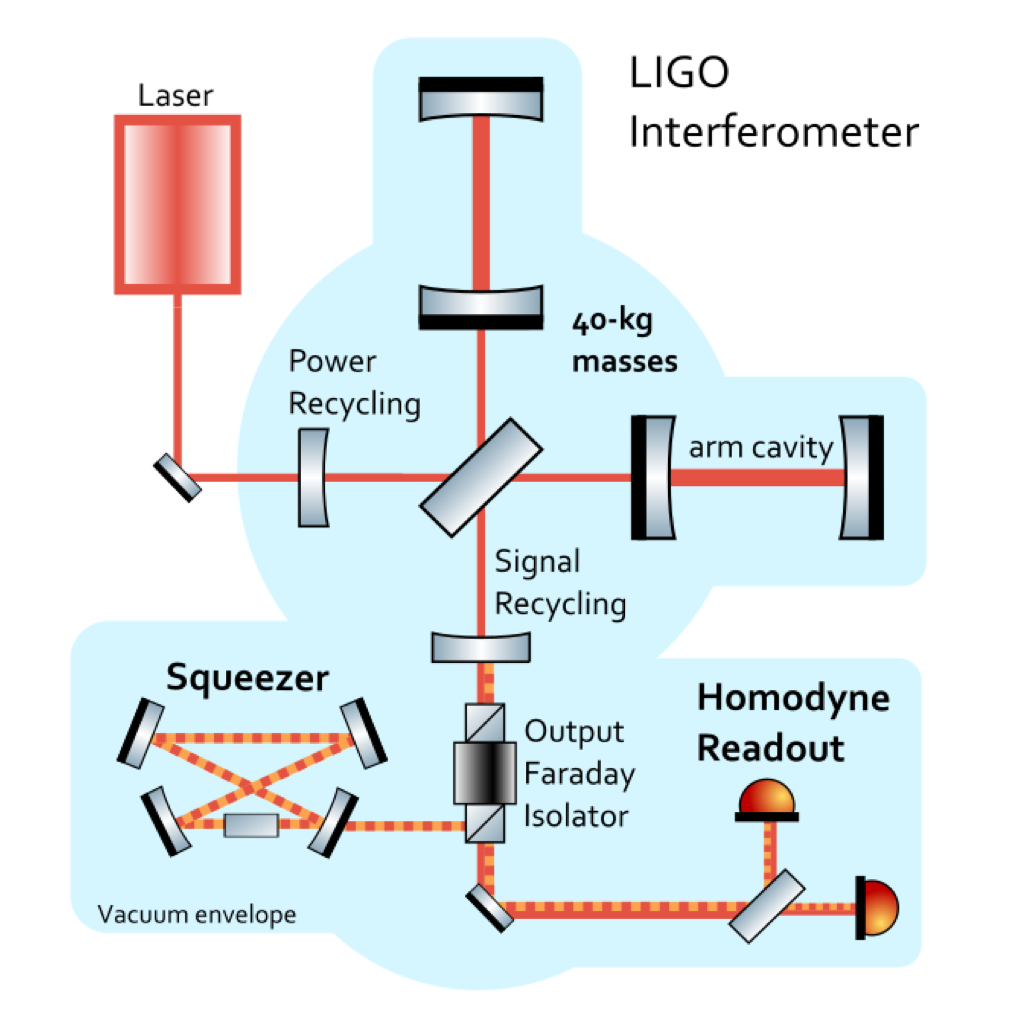
\includegraphics[scale=0.5]{interferometer}
          \centering
          \caption{Simplified schematic of the experimental setup. Several modifications to the Michelson interferometer are shown such as power and signal recycling. The photodetector records the differential lengths of the arms. \cite{9}}
          \label{fig:interferometer}
        \end{figure}

\subsection{Ground-Based Laser Interferometers}

	Detectors have nearly $4\pi$ steradian sensitivity to events over the sky. 
	This means that any source on the sky will be detectable,
        not just sources in specific pointing directions.

	A single interferometer is unable to detect GW alone,
	because it us difficult to separate a signal from noise confidently 
	and also provides no directional information about the source.
	A worldwide network of detector is essential to a successful GW detection:
	looking for identical, simultaneous signals from multiple detectors worldwide, 
	rules out noise sources which are local to a given detector. 
	More detectors means a better determination of the direction of GW sources: 
	to reconstruct the location of a transient signal is primarily due to triangulation 
	based on the observed time delays of the signal at several detectors. 
	For more than two sites, requiring a consistency between the observed amplitudes 
	will also serve to restrict the allowed sky positions\cite{12}.

	A crucial aspect of the research is to make the instrument sufficiently sensitive:
        at the targeted strain sensitivity of $10^{−21}$ m, the resulting arm length change is only $ 10^{-18}$ m for km-scale instruments, that is
        a thousand times smaller than the diameter of a proton.
        A key feature of the detectors is simply their scale:
        the arms are made as long as practically possible to increase the signal due to a GW strain.

	We now briefly list current GW interferometers.
	\begin{itemize}
        \item LIGO. LIGO operates two identical and far apart GW observatories: 
          LIGO Hanford Observatory (LHO), in Washington, and LIGO Livingston Observatory (LLO), in Louisiana.
          The sites are separated by roughly 3000 km, 
          and are situated to support coincidence analysis of events.
          LIGO's original instrument engaged in "science observations" from 2002 to 2010. 
          During this initial phase, the Hanford site operated two collocated interferometers:
          one detector with 4 km long arms (H1) and another with 2 km long arms (H2). 
          The Livingston site operated a second 4 km detector (L1). 
          Each observatory is made up of ultra high vacuum system, 
          where the interferometer is placed.

          This Advanced LIGO project successfully improved the capabilities of the detectors, 
          both interferometers were completely overhauled to incorporate much more sophisticated engineering.
        \item Virgo. The Advanced Virgo detector, located in Cascina (near Pisa) in Italy, 
          is the upgraded version of the Virgo detector. 
          As LIGO, it is a Michelson interferometer but with 3 km arms.
        \item GEO600. GEO600 is a 600 m interferometer located near Hannover,
          Germany. It is designed and operated by scientists from the
          Max Planck Institute for Gravitational Physics and the Leibniz Universität Hannover.
        \item KAGRA. It is Japan’s first GW detector and also the first GW detector to operate
          at cryogenic temperatures, improving sensitivity at frequencies around 100 Hz.
        \end{itemize}

\section{Interaction of Gravitational Waves with Test Masses}
	The effects of GWs cannot be seen in isolated bodies. 
	This is a result of the fact that a single test mass, 
	in a frame freely falling with it, will remain at rest.
	At least two test masses are required to measure the effects of GWs. 	
	This is also the case when one wants to measure any curvature of spacetime.
        Therefore, to understand how GWs interact with the interferometric detectors,
        it is necessary to use the geodesic equation and the geodesic deviation equation, which are also important tools
        for understanding the physical meaning of a given gauge choice \cite{3}. 
        In fact the physics must be invariant under coordinate transformations but GWs and the detector description's depend on the chosen reference frame.
        Consider a test mass initially at rest at $\tau = 0$.

	The geodesic equation then becomes
        \begin{equation}
          {{dx^i}\over{d\tau^2}} = -[\Gamma^i_{\nu\rho}{{dx^{\nu}}\over{d\tau}}{{dx^{\rho}}\over{d\tau}}]_{\tau=0} \\ 
          = - [ \Gamma^i_{00}({{dx^0}\over{d\tau}})^2]_{\tau=0}
        \end{equation}
        because
        \begin{equation}
          {{dx^i}\over{d\tau}} = 0 \hspace*{2cm} at \hspace*{0.5cm}\tau = 0
        \end{equation}
        since the mass is initially at rest. Expanding to first order in $h_{\mu\nu}$,
        the Christoffel symbol $\Gamma^i_{00} = 1/2(2\partial_{0}h_{0i} - \partial_i h_{00})$ vanishes in the TT gauge
        because both $h_{00}$ and $h_{0i}$ are set to zero by the gauge condition.
        Therefore, if at time $\tau = 0$ $dx^i/d\tau$ is zero, it remains zero at all times,
        because its derivative also vanishes.
        This shows that if two test masses are initially separated by a coordinate separation of $x^i$ in the TT frame,
        and are at rest with respect to each other, they will remain at this separation.
        Overall, it seems that a GW has no influence on the geodesic or on the deviation of geodesics. 
        In other words, in the TT gauge the coordinate location of a slowly moving, free-falling body is unaffected
        by a GW because the coordinates move with the waves \cite{4}.

        The TT gauge illustrates that, in general relativity, the physical effects are not expressed by what happens
        to the coordinates since the theory is invariant under coordinate transformations:
        the position of test masses does not change because the gauge freedom allowed to define the coordinates
        in such a way that they do not change \cite{3}.
        Physical effects can instead be found monitoring proper distances, or proper times. 
        GWs cause the proper separation between two freely falling particles to oscillate,
        even if their coordinate separation is constant. Consider two  free-falling particles,
        located at $z = 0$, and separated on the $x$ axis by a coordinate distance $L_c$.

        Consider a GW in TT gauge that propagates down the $z$ axis, $h^{TT}_{\mu\nu}(t,z)$.
        The proper distance L between the two particles in the presence of the GW is given by
        \begin{align}
          \label{distance}
          L & = \int^{L_c}_{0}{dx\sqrt{g_{xx}}} = \int^{L_c}_{0}dx\sqrt{1 + h^{TT}_{xx}(t,z=0)} \\
          & \simeq \int^{L_c}_{0}{dx[1 + {1 \over 2}h^{TT}_{xx}(t,z=0)]} \\
          &= L_c[1 + {1 \over 2}h^{TT}_{xx}(t,z=0)]
        \end{align}
        Therefore, the proper distance expands and shrinks periodically, with a fractional length change $\delta L/L_c$ given by
        \begin{equation}
          {{\delta L}\over{L_c}} \simeq {1 \over 2} h_{xx}^{TT}(t,z=0)
        \end{equation}
        Even though this result is calculated in the TT gauge, it is indeed gauge independent;
        $h_{xx}^{TT}$ acts as a strain, a fractional length change.
        Because the time that light travels between the two test masses is related to the proper distance,
        which directly relates to the accumulated phase measured by laser interferometric GW observatories,
        GWs leave an imprint on the time it takes for a photon to make a round trip \cite{4}.

        Consequently, interferometers can potentially measure these imprints by measuring the length difference between
        their arms. The “extra” phase $\delta \phi$ (if $L \ll \lambda$ so that the metric perturbation
	does not vary during a light travel time) accumulated by a photon that travels
        down and back the arm of a laser interferometer in the presence of a GW is $\delta \phi = 4\pi \delta L \lambda$,
        where $\lambda$ is the photon’s wavelength and $\delta L$ is the distance
        the end mirror moves relative to the beam splitter.

\subsection{Local Proper Reference Frame}
        Since positions in a lab are not marked by test particles,
        the $TT$ frame is not very practical.
        The preferred reference frame is the proper detector frame
        in which the test particle is free to move because of a passing GW.
        The path of a test particle can then be described by Newtonian equations of motion in terms of forces.
        There are terms proportional to the Riemann curvature tensor from the gravitational field of the Earth
        but also terms from static gravitational forces, Coriolis forces, etc \cite{5}.
	GW detectors need to be designed in order to maximise their sensitivity to the part proportional to the Riemann tensor while minimizing their sensitivity to all other terms.
        Consider a detector capable of measuring changes in the proper distance, between two test masses
        and assume the detector has a characteristic size that is much smaller
        than the characteristic wavelength of the GW.

        In this case, one can approximate the entire detector to be in a near local Lorentz frame
        (freely falling frame), even in the presence of GWs. This coordinate system is defined by the requirements
        \begin{equation}
          z^i(\tau) = 0, \hspace*{2cm} g_{ab}(t, 0) = \eta_{ab}, \hspace*{2cm} \Gamma^a_{bc}(t,0) = 0,
        \end{equation}
        which imply that the metric has the form
        \begin{equation}
          ds^2 \approx -dt^2 + \delta_{ij}dx^i dx^j + O({{x^ix^j}\over{L^2_B}})
        \end{equation}
        where $L^2_B$ denotes the typical variation scale of the metric.

        Consider now the proper distance between the two geodesics of the test masses, $\zeta^i$.
        The GWs influence these two test masses via the geodesic deviation equation
        \begin{equation}
          {{d^2\zeta^{\mu}}\over{d\tau^2}} + 2\Gamma^{\mu}_{\nu\rho}{{dx^{\nu}}\over{d\tau}}{{dx^\rho}\over{d\tau}} + \zeta^{\sigma}\Gamma^{\mu}_{\nu\rho,\sigma}{{dx^{\nu}}\over{d\tau}}{{dx^{\rho}}\over{d\tau}} = 0
        \end{equation}
        Assuming the two test masses are moving non-relativistically, $dx^i/d\tau$ can be neglected compared to $dx^0/d\tau$.
        Furthermore, the term proportional to $\Gamma^{\mu}_{\nu\rho}$ is negligible compared to other terms in a near  local-Lorentz frame, LLF. Hence,
        \begin{equation}
          {{d^2\zeta^{\mu}}\over{d\tau^2}} + \zeta^{\sigma}\Gamma^{i}_{00, \sigma}({{dx^0}\over{d\tau}})^2 = 0
        \end{equation}
        Further simplifying $\zeta^{\sigma}\Gamma^{i}_{00, \sigma} \approx \zeta^{j}\Gamma^{i}_{00, j}$
        \begin{equation}
          {{d^2\zeta^{\mu}}\over{d\tau^2}} + \zeta^{j}\Gamma^{i}_{00,j}({{dx^0}\over{d\tau}})^2 = 0
        \end{equation}
        But in the LLF, $R^i_{0j0} = \Gamma^i_{00,j} - \Gamma^i_{0j,0} = \Gamma^i_{00,j}$ and therefore
        \begin{equation}
          {{d^2\zeta^{\mu}}\over{d\tau^2}} + R^i_{0j0} \zeta^j({{dx^0}\over{d\tau}})^2 = 0
        \end{equation}
        Because $dx^0/d\tau \approx 1$, one can approximate $\tau \approx t$:
        \begin{equation}
          {\ddot \zeta}^j = - R^i_{0j0}\zeta^j
        \end{equation}
        The key quantity entering into the equation, the Rienmann tensor, is gauge invariant in the linearized theory and
        it can be evaluated in any convenient coordinate system.

        The expression for the Rienmann tensor in terms of the TT gauge metric perturbation $h_{ij}^{TT}$ is
        \begin{equation}
          R^i_{0j0} = R_{i0j0} = - {1 \over 2}{\ddot h}_{ij}^{TT}
        \end{equation}
        Substituting into the previous equation, the geodesic deviation equation in the proper detector frame takes the form
        \begin{equation}
          {\ddot \zeta}^i = {1 \over 2}{\ddot h}_{ij}^{TT}\zeta^j
        \end{equation}
        which can be interpreted as if the influence of a GW in a near LLF resembles a Newtonian force.
        Generalizing Eq.\,(\ref{distance}), the proper distance may be written as
        \begin{equation}
          s = \sqrt{L^2 + h_{ij}(t)L_{i}L_{j}}
        \end{equation}
        where $L_i$ denotes the spatial separation between two test masses and $L$ the associated coordinate distance.
        In the given metric for the proper reference frame, the proper distance is just $|L| = \sqrt{L_iL_j}$ up to fractional errors;
        since we are considering detectors such that
        $L \ll \lambda$, these errors are smaller than the fractional distance changes caused by the GW.
        Therefore, $|L|$ is simply identified as the proper separation. The equation for analyzing an interferometric GW detector is therefore
        \begin{equation}
          {\ddot L}^i = {1 \over 2}{\ddot h}_{ij}^{TT}L^j
        \end{equation}

\subsection{Ring of Test Masses}
        Consider a ring of test masses in the $(x, y)$ plane of a proper detector frame, initially at rest, centred at $z = 0$,
        and a GW travelling in the $z$-direction.
        This situation restricts the attention to the $(x,y)$ plane alone, because $h_{ij}^{TT}$ is transverse to the propagation direction,
        so the GW will only have influence in the plane of the test masses:
        the only non zero compontents of the metric perturbation are
        \begin{equation}
          h_{xx}^{TT} = - h_{yy}^{TT} = h_{+} \hspace*{3cm} h_{xy}^{TT} = h_{yx}^{TT} = h_{\times}
        \end{equation}
        where $h_{+}=h_{+}(t-z)$ and $h_{\times}=h_{\times}(t-z)$ are the two polarisation components, which are independent and can be considered separately.
        For the plus polarisation at $z=0$ and initial conditions $h_{ij}^{TT} = 0$ at $t=0$:
        \begin{equation}
          h_{ab}^{TT} = 
          \begin{bmatrix}
            1  & 0 \\
            0 &  -1 \\
          \end{bmatrix} 
          h_{+}\cos \omega t
        \end{equation}
        If the displacement between geodesics is $\zeta_a (t) = (x_0 + \delta x(t), y_0 + \delta y(t))$, then
        \begin{equation}
          \delta {\ddot x} = - {{h_{+}} \over 2} (x_0 + \delta x) \omega ^2 \sin \omega t
        \end{equation}
        \begin{equation}
          \delta {\ddot y} =  {{h_{+}} \over 2} (y_0 + \delta y) \omega ^2 \sin \omega t
        \end{equation}
        Assuming that the perturbations are $O(h)$, and thus small compared to the unperturbed locations, $\delta x$ and $\delta y$ can be neglected.
        The integrations gives the deviations caused by the plus polarisations:
        \begin{equation}
          \delta x(t) =  {{h_{+}} \over 2} x_0 \sin \omega t
        \end{equation}
        \begin{equation}
          \delta y(t) = - {{h_{+}} \over 2} y_0  \sin \omega t
        \end{equation}
        Similarly, for the cross polarisation at $z=0$ and initial conditions $h_{ii}^{TT} = 0$ at $t= 0$, the situation is described by the equations
        \begin{equation}
          \delta x(t) =  {{h_{\times}} \over 2} y_0 \sin \omega t
        \end{equation}
        \begin{equation}
          \delta y(t) =  {{h_{\times}} \over 2} x_0  \sin \omega t
        \end{equation}
        This set of equations describes the changes in the $x$ and $y$ components for a passing GW.
        The plus polarisation alternately stretches and compresses the ring of test masses in the x and y directions,
        while the cross polarisation exhibits the same behaviour rotated by $\ang{45}$ in the $x - y$ plane. This is shown in Figure 2.1.
        \begin{figure}[t]
          \label{ring}
          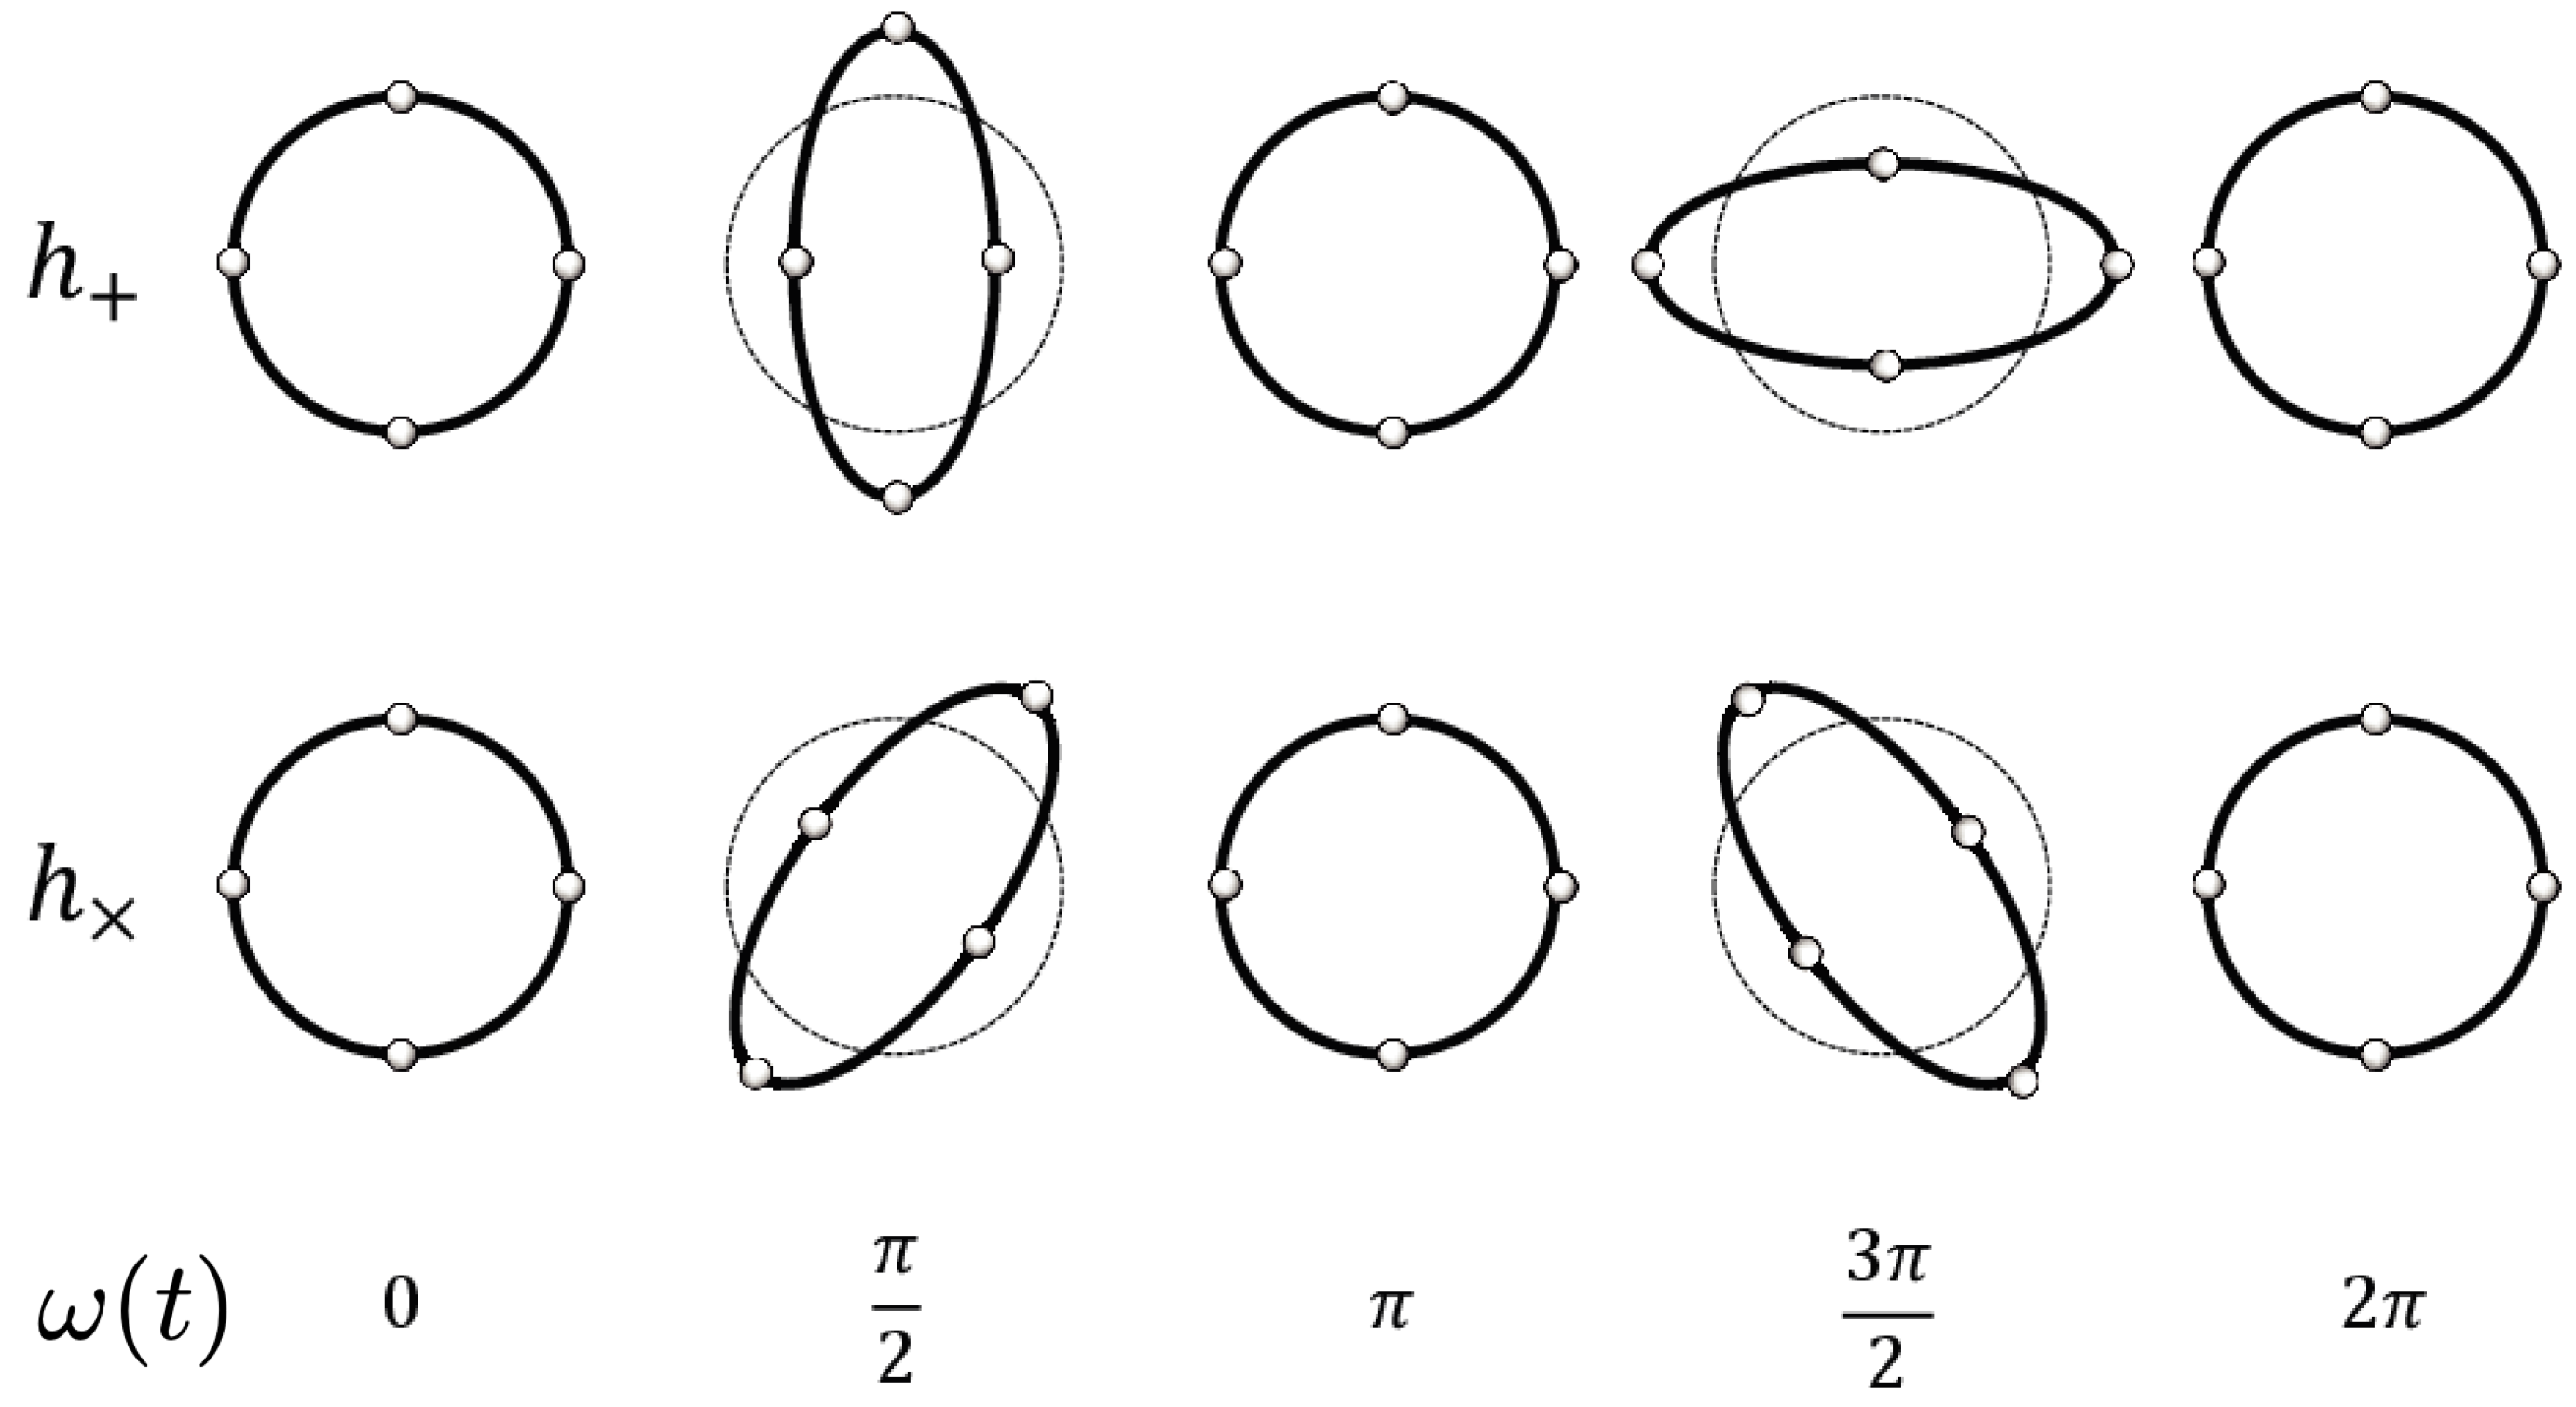
\includegraphics[scale=1]{ring}
          \centering
          \caption{The effects of plus and cross polarisation on a ring of test masses. The plus polarisation alternately compresses and stretches the x- and y-separations. The cross polarisation has the same effect only rotated by  $\ang{45}$.}
          \label{fig:ring}
        \end{figure}

\section{Response of an Interferometer to a Gravitational Wave}
        Interferometers are sensitive to the relative difference between two distances, the so-called strain \cite{6} .
        Suppose we have an interferometer with its arms pointing along the unit vectors $u^i$ and $v^i$. The strain $h(t)$ is given by
        \begin{equation}
          h(t) = {1 \over 2} (h_{ij}u^iu^j - h_{ij}v^iv^j) = D^{ij}h_{ij}(t)
        \end{equation}
        where $D^{ij}$ is referred to as the detector tensor and is given by
        \begin{equation}
          D^{ij} = {1\over 2} (u^iu^j -v^iv^j)
        \end{equation}
        As the expression for $h(t)$ is linear in $h_{+}$ and $h_{\times}$, one can also write
        \begin{equation}
          \label{beampattern}
          h(t) = F_{+}h_{+} (t) + F_{\times}h_{\times}(t)
        \end{equation}
        where $F_{+,\times}$ are called the beam pattern functions. Suppose we have a detector
        with arms that are perpendicular to each other, one pointing in the x-direction and the other
        in the $y$-direction in a Cartesian coordinate system. This detector frame, denoted by $(x,y,z)$,
        is generally different from the GW coordinate system, denoted by $(x^\prime,y^\prime,z^\prime)$, where the source
        is conveniently described. To account for such a difference, we first note that when the plus
        and cross polarisations are not equal in strength, we can rotate the coordinate system by
        an angle $\psi$ around the $z^\prime$ axis so that the $x^\prime$ and $y^\prime$ axes
        coincide with the mayor and minor axis of the associated ellipse.

        In going from the GW frame to the detector frame, we can rotate the GW frame by
        an angle $\theta$ around the $x^\prime$ axis and an angle $\phi$ around the $z^\prime$ axis,
        where the angles $(\theta, \phi)$ denote the direction of propagation of the GW in the detector frame.
        Applying these three rotations, the beam pattern functions for a detector with perpendicular arms are given by
        \begin{align}
          F_{+}^{\ang{90}}& = {1 \over 2} (1 + \cos^2 \theta)\cos 2\phi \cos 2 \psi - \cos \theta \sin2\phi \sin2\psi \\
          F_{\times}^{\ang{90}}& = {1 \over 2} (1 + \cos^2 \theta)\cos 2\phi \sin 2 \psi + \cos \theta \sin2\phi \cos2\psi
        \end{align}
        

\section{Non-Stationary Transient Noise Sources}
	The various noises of the detector can be conveniently characterised by a spectral strain
        sensitivity with dimensions of $1/\sqrt{Hz}$, as we explain in this section. 
        The detector output $s(t)$ is composed of instrumental noise $n(t)$ arising from
        naturally occurring random processes and a potential strain signal $h(t)$
        \begin{equation}
          s(t) = n(t) + h(t)
        \end{equation}
        The detection problem then becomes how to distinguish $h(t)$ from $n(t)$ when $h(t) << n(t)$.
        In a way, $n(t)$ provides a measure of how small an $h(t)$ we can detect.
        Thus we take $n(t)$ as the detector’s noise and have a convenient way to
        compare performances of different detectors.
	The instrument response $s(t)$ can be also expressed as a convolution of the antenna patterns 
	with the two GW polarisations $h_{+}, h_{\times}(t)$:
        \begin{equation}
          s(t) = n(t) +  F_{+}h_{+} (t) + F_{\times}h_{\times}(t)
        \end{equation} 
	The antenna patterns depend on the frequency and sky location of the source; 
	for wavelengths that are large compared to the detector, the antenna patterns are simple quadrupoles \cite{19}.
	The information contained in the time series is usually represented in the Fourier domain 
	as a strain amplitude spectral density, $h(f)$.
	This quantity is defined in terms of the power spectral density $S_s(f) = \tilde s^{*}(f) \tilde s(f)$
	of the Fourier transform of the time series:
        \begin{equation}
          \tilde s(f) = \int^{\infty}_{-\infty} e^{-2 \pi ift} s(t)dt
        \end{equation}
	The strain amplitude spectral density is then defined as $h(f) = \sqrt{S_s(f)}$.
	Noise is categorised as either displacement noise, which directly moves the suspended mirrors
        causing a differential change in the arm cavity lengths, or as sensing noise,
        which appears in the readout signal but is not caused by a GW.

        We describe the principal noises that dominate the limits of our sensitivity, (Fig.\,\ref{fig:noise2}).
        \begin{figure}[t]
          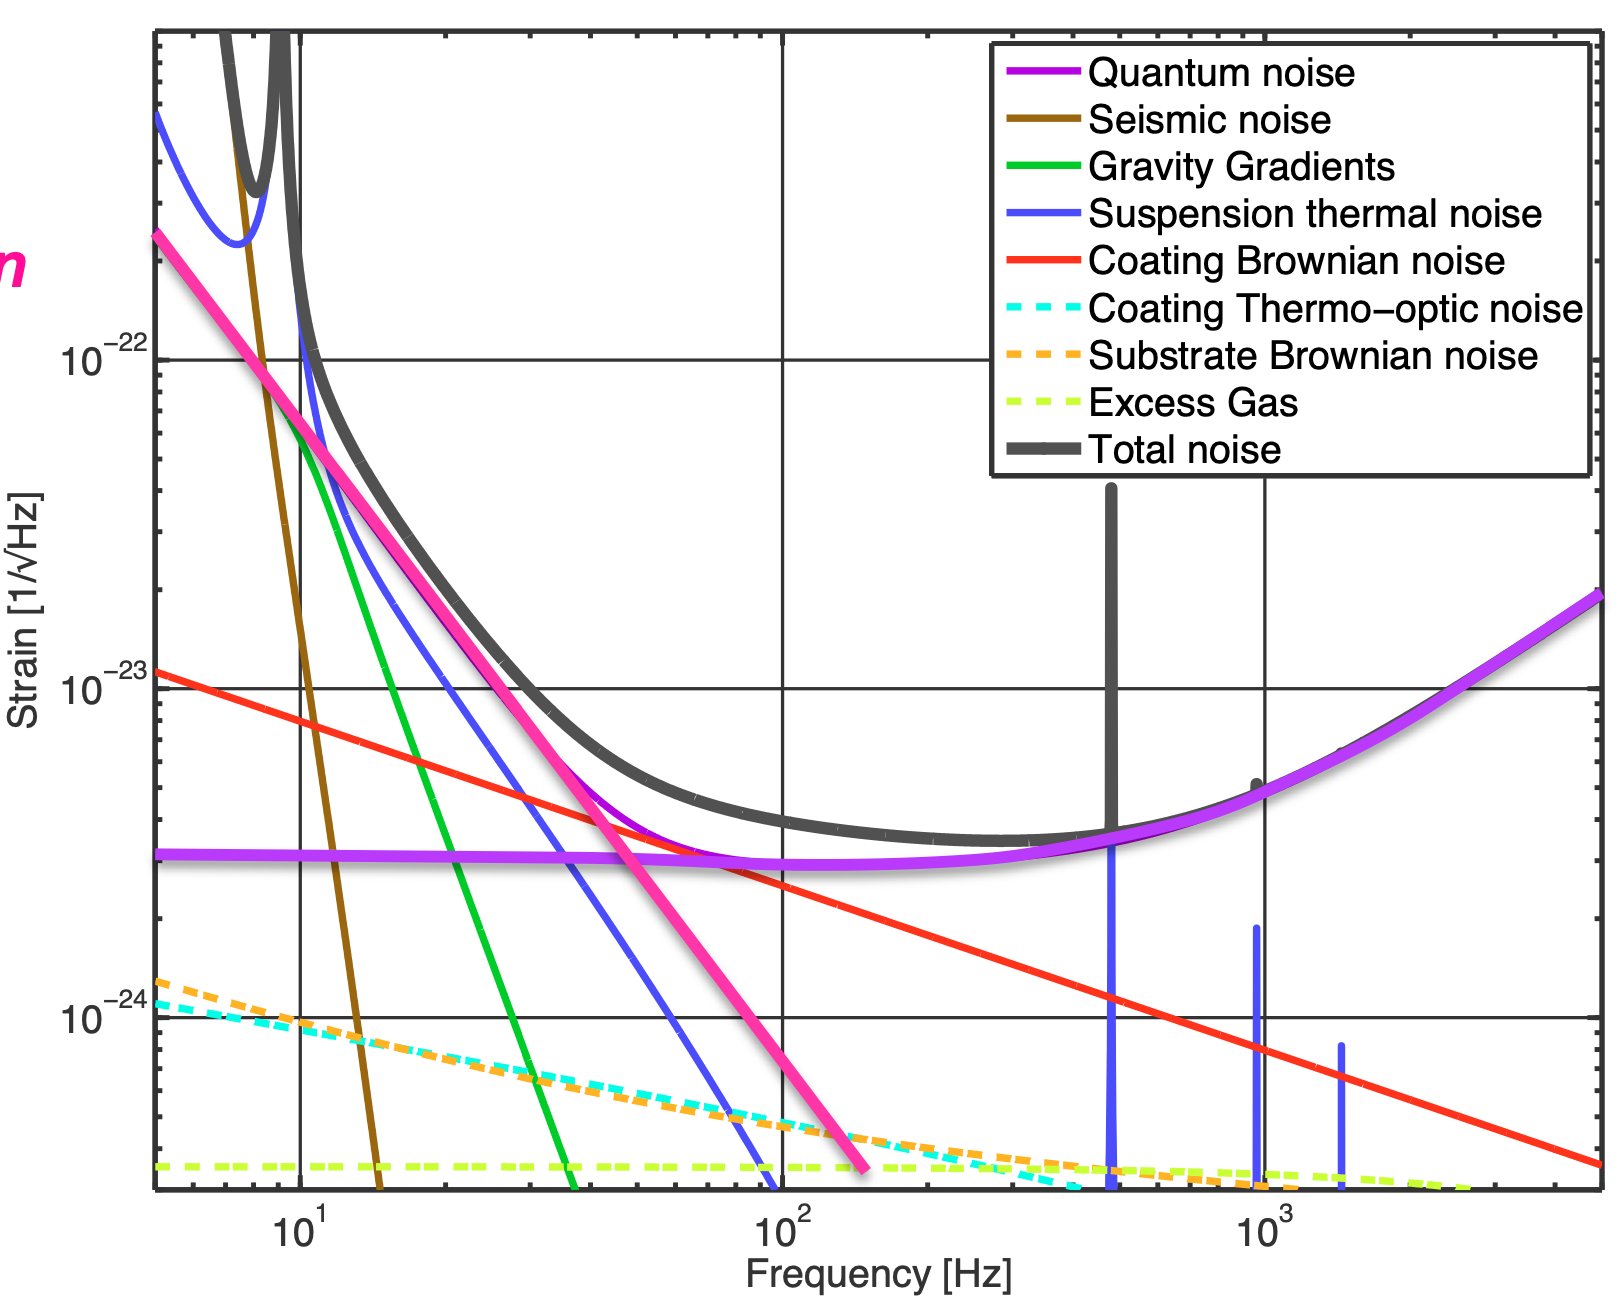
\includegraphics[scale=0.3]{noise2}
          \centering
          \caption{The strain equivalent spectral amplitudes $\sqrt{S_n(\omega)}$ of several noises couple to the detector. Most relevant contributions comes from quantum noise and from thermal noise of mirror coating and suspensions. Seismic noise dominates below 10Hz}
          \label{fig:noise2}
        \end{figure}
        At lower frequencies, up to 10Hz, the main contribution to the global noise
        is due to vibrations of the ground which couple to the mirror motion, (Fig.\,\ref{fig:noise2} brown line): 
	it shakes the optics and produces strain signals that mask GW signals. 
        This seismic noise is caused by earthquakes, weather and human activity.
        To reduce the potential movements of the optical elements,
        the mirrors are isolated using an advanced suspension system.

        At frequencies where the seismic motion has been sufficiently reduced,
        between 10Hz and 500Hz, the random Brownian motion of the molecules on the surface of the mirrors and wires dominates (Fig.\,\ref{fig:noise2}, red line).

        The thermal energy of the interferometer’s components induce vibrations both in the suspensions and in the mirrors.
        The nature of GW signal requires the sensitivity of the interferometric detectors
        to be extremely high in broad frequency band.
        Therefore, the power spectrum density of the thermal noise must be considered in the development of the detectors.
        The Fluctuation-dissipation Theorem relates the spectrum of the thermal noise to the amount of dissipation
        \begin{equation}
          S_{n}(\omega) = - {{4k_bT} \over {\omega}} Im[H(\omega)]
        \end{equation}
        From this equation is possible to state that the energy of fluctuations has a frequency dependent distribution;
        $H(z)$ is the transfer function of the system, it is a mathematical function that models the device’s output, defined as
        \begin{equation}
          H(x) = {1 \over {iWZ(\omega)}}
        \end{equation}
        In which $Z(\omega)$ is the impedance of the system in the frequency domain that can be computed as the ratio
        between the Fourier components of the generalised force $\tilde F(\omega)$ and the response of the system $\tilde X(\omega)$
        \begin{equation}
          Z(\omega) = {{\tilde F(\omega)} \over {i\omega \tilde X(\omega)}}
        \end{equation}
        In the case of an harmonic oscillator, the noise spectral density is
        \begin{equation}
          S_n(\omega) = {{4k_bT} \over {m\omega}} {{{\omega_0}^2 \phi(\omega)} \over {(\omega^2-{\omega_0}^2)^2 + {\omega_0}^4 \phi^2(\omega)}}
        \end{equation} 
	Generally, thermal noise can be reduced decreasing the dissipation with monolithic suspensions and better coatings
        other than lowering the temperature using cryogenic payloads as it is done in KAGRA.
        Quantum mechanics limits the precision at which the test mass positions can be determined.

        At high frequencies, photon shot noise limits the sensitivity, 
	while at low frequencies it is limited by radiation pressure.
        The photon shot noise is produced by the natural fluctuations in the rate of photons arriving at the photodiode,
        that follow a Poisson process. The noise will decrease with increasing laser power,
        recycling cavity gain, arm cavity gain, and arm length.
        The corresponding noise spectral density is
        \begin{equation}
          S_n(\omega) = \Bigg({{\lambda_{laser}} \over {4 \pi L}}\Bigg)^2 {{2 \hbar \omega_{laser}} \over {P}}
        \end{equation}
        Radiation pressure noise is associated with the photons from the laser striking the mirror
        and causing a force on the mirror. Of course, increasing the laser power to combat shot noise
        will actually result in an increase of radiation pressure.
        \begin{equation}
          S_n(\omega) =  {{32 \hbar \omega_{laser}P} \over {(4MLc \pi^2 f^2)^2}}
        \end{equation}
        This is an example of the Heisenberg’s Uncertainty Principle, which says that the knowledge
        of the position and the momentum of a body is restricted from the relation $\Delta x \Delta p \geq \hbar$. 
        The high laser power required to determine the position of the test masses exerts
        a fluctuating radiation pressure which perturbs the test mass positions. 
        The minimum noise level is called Standard Quantum Limit (SQL) and sets a fundamental limit
        on the sensitivity of beam detectors, contributing to the noise as
        \begin{equation}
          S_n(\omega) = {{2 \hbar} \over {M(\pi f L)^2}}
        \end{equation}
        Moreover, the presence of residual gas in the beam tubes would worsen the performance
        of the mirrors and of the laser; for this reason the vacuum system is maintained at a pressure
        of below $10^{-6}$Pa and the noise curve of the interferometer includes only
        the most dominant residual gas component, hydrogen, at a pressure of $10^{−7}$ Pa. 
        \begin{figure}[t]
          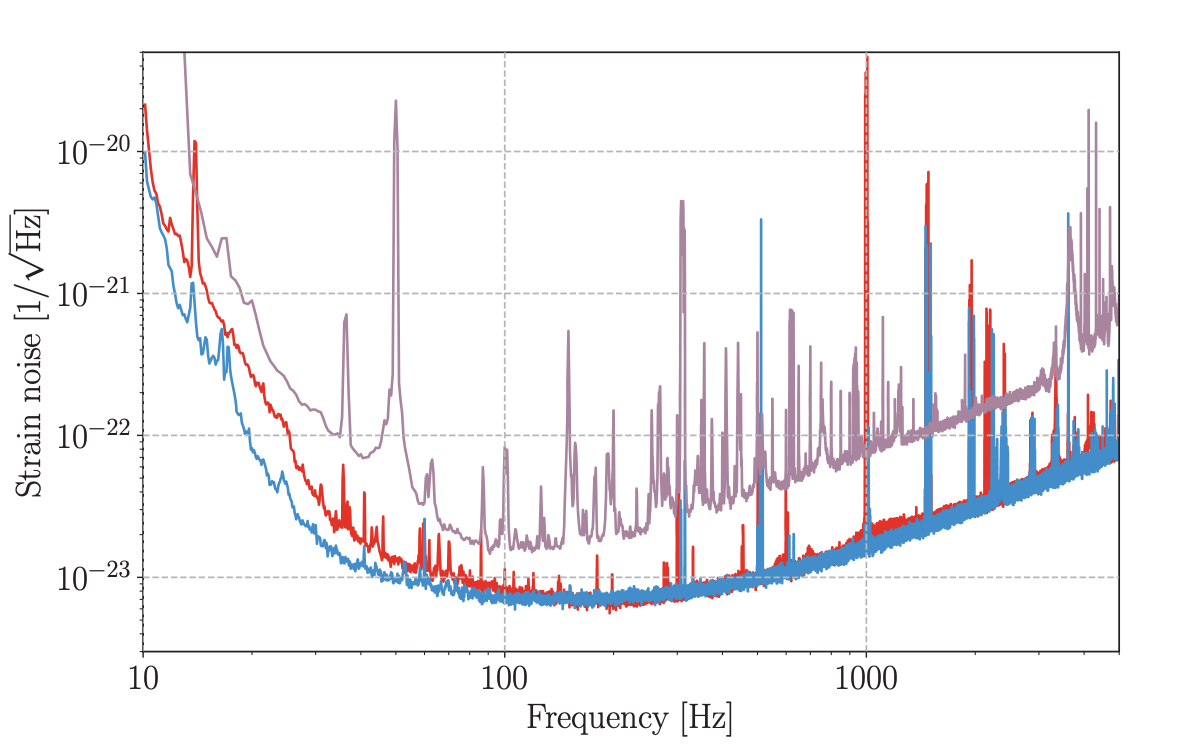
\includegraphics[scale=0.6]{noise1}
          \centering
          \caption{Amplitude spectral density of the total strain noise  of the Virgo, LHO, and LLO detectors. The curves are representative of the best performance of each detector during O2 \cite{13}.}
          \label{fig:noise1}
        \end{figure}

\subsection{Sources}
\label{sec:sources}
	There are four different classes of physical sources 
	that are potential sources of GWs 
	of sufficient amplitude to be detectable 
	by current or theorised GW detectors. 

\subsubsection{Compact Binaries Coalescences}
	Compact binary star systems, in which each member is a NS or BH, 
	are currently the only observed sources of GWs.
	They are an ideal source for ground based GW detectors, 
	as their compactness allows their orbital separation to become 
	small enough before they merge for them to emit GWs in the detectors sensitive frequency band.
	If one of the components of the binary is a NS 
	then there may be an electromagnetic counterpart to the GW signal \cite{20}. 
	The loss of energy from the system will cause the orbital radius to decay, 
	the frequency to increase, and the amplitude of the radiation to increase, 
	producing a distinctive chirp-like signal. 
	Eventually, the two objects will be close enough to merge together, 
	and the new single object will pulsate in an excite state as it tries to return to equilibrium \cite{21}. 
	If the remnant is a BH, this phase is known as the ringdown phase and it is well-modelled as a series of quasi-normal modes. 
	As the form of the gravitational radiation can be predicted allows 
	a more sensitive search to be performed: knowing the form of the signal 
	that is being search for allows powerful matched filtering techniques 
	and signal consistency tests to be used in the attempt to detect such signals.

\subsubsection{Bursts}
	A burst of GWs is an event that releases a large amount 
	of gravitational energy over a very short period of time, typically less than a few seconds.  
	Astrophysical events that are believed to result in a transient signal 
	include gamma ray bursts and supernovae explosion as well as the final stages of a coalescing binary. 
	GW signal with a partially modelled or unknown waveform, 
	this may be due to unknown or complicated physics, or the source may be something totally unpredicted. 
	The matched filtering is not a useful technique to search for this type of signal, 
	as the waveform of a GW burst signal is unknown \cite{3}. 
	Searches for GW bursts typically search for excess power that occurs coherently between multiple detectors.  
	Even with no knowledge of the source of a GW signal, 
	it is still possible to estimate some of the source parameters. 
	Searches for GW bursts typically give estimations of the duration, 
	amplitude and frequency of the source.

	An estimation of the sky position is given by measuring the difference 
	in arrival time between different detectors. 
	If the distance to the source is known, 
	perhaps through an electromagnetic counterpart, 
	then it is possible to estimate the energy of the source. 

\subsubsection{Continuous Sources}
	A periodic source is a source that emits at constant or nearly constant frequency.
	The prototypical source of continuous GWs is high frequency rotating NSs 
	with a non-axial deformation or low frequency binary systems 
	composed of white dwarfs or BHs far from merger. 
	These sources should be present throughout the operational lifetime of a detector, 
	so the greater the observation time, the better the sensitivity to periodic sources becomes. 
	Spinning NSs will lose energy and spin down over time, 
	and this energy loss is due to a number of different mechanisms, 
	including emission of gravitational radiation \cite{3}. 
	To emit a continuous GW with characteristic amplitude, 
	a NS must have a non-axisymmetry in the crust. 
	The radiation amplitude is proportional to the crucial parameter $\epsilon$, 
	the fractional asymmetry that is proportional to the mass of the bump on the surface.

	As NSs emit electromagnetic radiation, 
	it is possible to target searches of GWs for NSs with positions, 
	frequencies and spin-downs known from X-ray, radio and gamma-ray observations. 
	Examples are the Crab and Vela pulsars. 
	Continuous GWs have not yet been detected, 
	but current searches have produced upper limits for their emission. 
	Upgraded interferometers in LIGO could set an upper limit on  
	$\epsilon$ of order $10^{-6}$ for sources at $\sim10$ kpc, 
	and explain how a NS can be distorted to give a value of $\epsilon$ that is interesting as a GW source. 
	Whatever the mechanism generating the distortion, 
	it is clear that  $\epsilon$ will be small,
	so that $h \sim 10^{-24}$ or smaller, which is quite weak. 
	Measuring these waves will require
	coherently tracking their signal for a large number of wave cycles, 
	which is actually quite difficult, 
	since the signal is strongly modulated by the Earth’s rotation and orbital motion.

	Searching for periodic GWs means demodulating the motion of the detector, 
	a computationally intensive problem since the modulation is different for every sky position \cite{4}. 
	Unless one knows in advance the position of the source, 
	one needs to search over a huge number of sky position "error boxes”.

\subsubsection{Stochastic Background}
	Stochastic backgrounds are “random” GWs, 
	arising from a  number of sources that overlap 
	in time and frequency that are not individually resolvable \cite{22}. 
	The sum of the signals at any given time and frequency will have 
	a random pattern that may be analysed statistically but not predicted precisely.
	A particularly interesting source of stochastic waves is the dynamics of the early Universe, 
	which could produce an all-sky GW background, 
	similar to the cosmic microwave background.
	However, to measure waves from this epoch, 
	we would need much more sensitive detectors than the ground-based interferometers available.
	Stochastic backgrounds are usually idealized as being stationary, 
	isotropic and homogeneous and because of their random nature they look just like noise \cite{4}.	
	Another possible background could come from astrophysical sources.

	These possible sources include a population of rotating NSs 
	and a population of white dwarf binaries that would be important mostly for a space-based interferometers such as LISA. 

%----------------------------------------------------------------------------------------------------------------------------------------------------------------------------------------------------------
\chapter{Data Analysis for Coalescing Binary Systems}
\label{ch:datatools}
\fpg{Giri di correzione: 1.}%
	One of the tasks of GW data analysis is to extract GWs signal 
	buried into noisy interferometric strain data, hence achieving GW detections.
	The techniques involved in this proces depend on the type of source.
	GW searches from the inspiral, merger and ringdown phases of compact binary systems 
	are based on two broad techniques: 
	modelled searches which use theoretical waveforms for the GW emitted by such systems 
	as predicted by general relativity, and 
	unmodelled (or burst) searches which assume minimal information about these waveforms \cite{23}.
        This chapter provides a basic overview of the main data analysis ingredients needed to perform a modelled GW search:
        matched filtering, template banks, evaluation of a candidate's significance, measure of the sensitivity of a search.

\section{Matched Filtering}
\label{sec:matched_filtering}
	Although signals from coalescing binaries will most probably not stand above the broadband noise of the detector, 
	their detection is possible by the use of matched filtering, 
	which takes advantage of the fact that the waveform can be fairly well predicted. 
	As we will see, this technique is the optimal detection strategy when searching for GWs
        with well understood waveforms in Gaussian noise.

	The filtering procedure involves correlating the detector output 
	with a copy of the expected waveform, 
	called template.
	A real detector operates over a finite frequency band, 
	and acquires data at a finite sample rate \cite{24}. 
	In this case, the noise power spectrum $S_n$ 
	may be taken to be infinite outside the bandwidth of the instrument, 
	effectively restricting the range of integration to lie between $[-f_N, f_N]$, 
	where $f_N$ denotes the Nyquist frequency $f_N = 1/(2\Delta t)$, 
	and $\Delta t$ is the time between successive data samples.

	The measured detector strain amplitude, $s(t)$, may or may not contain a signal,
	thus it will be composed of $n(t)$, the real strain-equivalent noise
        produced by fluctuations within the detector and its environment, 
	and possibly a GW of known form, $h(t)$
        \begin{equation}
          \label{eq:strain}        
          s(t) = h(t) + n(t)\,.
        \end{equation}
        When no signal is present,   		
        \begin{equation}
          s(t) = n(t)\,.
        \end{equation}
        The aim of the match filtering is to look for a filter function to process the data,
	the output of which will be large when a signal is present and small otherwise. 
        If the waveform, $h(t)$, is embedded in stationary Gaussian noise with zero mean and one-sided power-spectral density (PSD) $S_n(f)$,
        the optimal filter takes the form $\tilde h_{\rm template}/S_n$, where $\tilde h_{\rm template}$
        is the frequency domain waveform template that approximates the real signal to the best of our knowledge.
	This optimal filter may be cross-correlated with the data over the detector frequency band to search for GW
        signals.  The output of this filtering operation may be viewed as a weighted inner product in the frequency domain, 
	between the data and the template, where the weight is the inverse PSD of the detector:
        \begin{equation}
          (s|h)(t) = 4Re \int^{f^{high}}_{f^{low}} {{\tilde s (f) \tilde h^{*}_{\rm template}(f)} \over {S_n (f)}} e^{2 \pi ift}df\,, 
        \end{equation}
	where the frequency limits $f_{low}$ and $f_{high}$ are determined by the detector bandwidth
	and $\hat s(f)$ denotes the Fourier-transformed detector data, defined as
        \begin{equation}
          \tilde s(f) = \int^{\infty}_{-\infty} s(t) e^{-2i \pi tf} dt\,.
        \end{equation}
        
\subsection{Signal-to-Noise Ratio}
	Finding the form of the filter which will optimally extract the signal from the noise,
        means locating the maxima of the output of the matched filter, $(s|h)(t)$, 
	over the arrival time and phase.
        One can therefore set a threshold value such that values of the matched filter 
	above it would indicate a signal candidate while values below would indicate the absence of signals.

	The filter output can be normalised by the variance of the optimal filter, $\sigma^2$,
	which is an estimate of the uncertainty in a measurement of $(s|h)$ due to the detector noise:
        \begin{equation}
          \sigma^2 =4 \int^{f^{high}}_{f^{low}} {{|\tilde h_{\rm template}(f)|^2} \over {S_n(f)}}df
        \end{equation}
 	The normalised output of the optimal filter is a new thresholding statistic and can be defined as  
	the signal-to-noise ratio (SNR), the ratio of the observed filter output to its,
        expected or observed, root-mean-square fluctuations \cite{24}:
        \begin{align}
          \rho(t) &= {{| (s|h) |} \over {\sigma_{h}}} \\
          &= {{(\tilde s|\tilde h_{\rm template})} \over {\sqrt{(h_{\rm template}|h_{\rm template})}}}\,.
        \end{align}
        The value of the SNR will then be proportional to the amplitude of the signal buried in the noise.
	The smart choice for a threshold that can be set on this value is such that
	it can admit as many signals as possible, while still keeping the false alarm rate low. 

\subsection{Matched Filtering for Compact Binary Coalescence Signals}
\label{subsec:mfcbc}
	An interferometric detector is sensitive to a linear combination 
	of the two GW polarisations \cite{26}: 
        \begin{equation}
          h(t) = F_{+}h_{+} (t) + F_{\times}h_{\times}(t)\,,
        \end{equation}
	where $F_{+}$ and $F_{\times}$ are the two antenna response functions of the detector, 
	which depend on $\theta$ and $\phi$, 
	the angular coordinates of the source sky position with respect to axes defined by the interferometer arms. 
	Due to the nature of GW signals from the inspiral stage of compact binary coalescences (CBCs), 
	it follows that the phase evolution of the cross polarisation is $\ang{90}$ out of phase with the plus polarisation:
        \begin{equation}
          h_{+}(t) = A(t) \cos (\phi (t))
        \end{equation}
        \begin{equation}
          h_{\times}(t) = A(t) \sin (\phi (t))  
        \end{equation}
	where $A(t)$ is the amplitude evolution of the signal 
	and $\phi(t)$ is the phase evolution of the signal. 
	The Fourier transform of the two polarisation are related by $\tilde h_{+} = i\tilde{h}_{\times}$, 
	which means that the inner product between the two orthogonal polarisations is zero 
        \begin{equation}
          (h_{\times}|h_{+}) = 0
        \end{equation}
	Hence, when filtering  $s = (Xh_{+}/\sigma_{h}) + (Y h_{\times}/\sigma_{h})$ 
	with the templates $h_{+}$ and $h_{\times}$, we obtain the matched-filter real-time series
        \begin{equation}
          z_{+} = X\sigma_{h}
        \end{equation}
        \begin{equation}
          z_{\times} = Y \sigma_{h} 
        \end{equation}
	This leads to the definition of the two-phase filter, 
	which has twice the degrees of freedom of a single-phase filter:
        \begin{equation}
          \rho = {1 \over \sigma_h} \sqrt{|z_{+}| ^2+ |z_{\times}|^2}
        \end{equation}
	The bonus of extracting information from both polarisations of the GW 
	comes at the cost of increasing the expectation value of $\rho$ when there is no signal present. 
	For a detector output that includes a signal at distance $D_{\rm eff}$, 
	$s(t) = n(t) + (D_{\rm eff}/1 Mpc)^{-1}h_{1Mpc}$, 
	a biased estimate of the effective distance for a given trigger 
	may be defined by combining the definition of the SNR with the template normalization $\sigma_h$:
        \begin{equation}
          \hat D_{\rm eff} = {{\sigma_h} \over {\rho}}
        \end{equation}
	In reality, the parameters of astrophysical systems will not be known a-priori, 
	and searches must therefore be sensitive to signals at any location in the parameter space \cite{25}. 
	Performing the matched-filter calculation at every point in the full parameter space 
	would be computationally prohibitive, 
	and therefore a number of analytic approximations are used to reduce the size of the parameter space. 
	It is assumed that the ``extrinsic'' parameters of a GW signal --- 
	sky-location, source orientation, polarisation phase and distance --- 
	can all be absorbed by applying a constant phase-shift, 
	constant time-shift and a constant amplitude scaling to the observed waveform \cite{27}. 
	With these assumptions in place, 
	one can analytically maximise over an overall amplitude and phase of the signal, 
	and use an inverse Fourier transform to quickly evaluate the statistic as a function of time.

	The component masses and spins --- the intrinsic parameters --- 
	are searched over by repeating the search process with a well chosen discrete set of waveform models 
	with varying values of the component masses and spins, 
	known as the template bank \cite{27}. 
	Physically, these assumptions hold if one assumes that the sources being observed 
	have negligible orbital eccentricity, precession and contributions from higher-order modes 
	to the GW signal \cite{23}. 

\section{Template Banks}
\label{sec:template_banks}
	To perform a matched-filtered search that recovers compact binary coalescence signals
	with minimal loss of SNR over a given range of intrinsic parameters, 
	one must filter the data against a predetermined collection of waveform models: the template bank \cite{28}.
	The manifold of waveforms is a continuous space in the component masses and spins. 
	One may only to search over this manifold on a discrete points, 
	which have to be placed in such a way that any signal
	that has parameters in the targeted space will still produce an SNR 
	above threshold by matching with the ''loudeest'' template \cite{27}.

	In order to compute the distance between two templates with different parameter values, 
	one can create a metric over the parameter space and then compute an ``error'' between two waveforms.
	Two neighbouring templates can be defined as $h(f;\lambda)$ and $h(f;\lambda + \Delta \lambda)$,
        where $\lambda = \{\lambda_{intr}, \lambda_{extr}\}$ is the set of
        intrinsic (masses and spins) and extrinsic (time and phase shifts) template parameters.
	The overlap of two waveforms, defined as the inner product inversely weighted by the detector one-sided  PSD $S_n(f)$, 
	can be written as  
        \begin{equation}
          (h_i| h_j)  \equiv 4 \int_{0}^{\infty} df {{\tilde h_i(f) \tilde h^*_j(f)} \over {S_n(f)}}.
        \end{equation}
	The normalised overlap between the two waveforms is given by
        \begin{align}
          (\hat{h}_i|\hat{h}_j)& = {{(h_i|h_j)} \over {\sqrt{(h_i| h_i)(h_j| h_j)}}}\,.
        \end{align}
	As the template waveforms are defined up to an overall normalization, 
	it is customary to work directly with the normalised $\hat{h}_i$'s. \\
	The match is then defined as
        \begin{equation}
          \mathcal{M}(\lambda, \Delta \lambda) \equiv \max_{\Delta \lambda_{extr}} (\hat h(f;\lambda), \hat h(f;\lambda + \Delta \lambda))
        \end{equation}
	The match is maximised only over the two extrinsic parameters of a template, 
	because waveforms related by time and phase offsets
	are described by the same template, 
	since all possible coalescence times and phases are searched for \cite{29}.

	This expression can be Taylor-expanded about $\Delta \lambda = 0$:
        \begin{equation}
          \mathcal{M}(\lambda, \Delta \lambda) \simeq 1 - g_{ij} \Delta \lambda^i \Delta \lambda^j\,,
        \end{equation}
	where 
        \begin{equation}
          g_{ij} \equiv -{1 \over 2} {{\partial^2\mathcal{M}} \over {\partial  \Delta \lambda^i  \partial \Delta \lambda^j}}\vert_{\Delta \lambda = 0}
        \end{equation}
	can be interpreted as a metric in the waveform manifold.  A commonly used quantity related to this metric
	is the mismatch between two templates $MM = (1 − \mathcal{M})$.
	Any mismatch between signal and template leads to a loss in SNR, 
	and to a down-weighting by the signal-based vetoes, see Sec.\,\ref{subsec:chi_square_test}.

        When constructing a template bank, this mismatch can be viewed as the means
	to compute the proper distance in the waveform space:
        \begin{equation}
          ds_{ij}^2 = 1 − \mathcal{M} = g_{ij} \Delta \lambda^i \Delta \lambda^j\,.
        \end{equation}
	This proper distance should be chosen to guarantee that the loss in SNR due to the mismatch 
	between template and signal does not jeopardize the detectability of the signal \cite{30}.

\subsubsection{Fitting Factor}
\label{subsec:fittingfactor}
	The standard measure used to determine the set of waveform models to used in a
        search is the fitting factor, $FF$.
	The fitting factor quantitatively describes the ``closeness'' of 
	the true signals to the template manifold, in terms of the fraction of 
	SNR obtained when filtering 
	the data with an approximate family of templates \cite{31}. 
	To quantify the bank coverage, usually Monte-Carlo simulations are carried out   
	to compute the distribution of fitting factors of the templates in the bank against 
	a set of injected signal waveforms with randomly chosen parameters \cite{32}.

	The fitting factor, $FF$, of a template bank with respect to an injected signal $h_{*}$ 
	is defined as the maximum value of match over all the templates:
        \begin{equation}
          FF(h_{*}) = \max_\Lambda \mathcal{M}(\tilde{h}_{*}, \tilde{h}(\Lambda))
        \end{equation}
	assuming that the signal model is the same for both templates and injections. 
	The fractional loss of SNR in capturing the signal 
	$h_{*}$ with the template bank is $1 - FF(h_{*})$.
	If the fitting factor is less than unity, the signal lies outside the parameter space, 
	and the fitting factor represents the cross-correlation between 
	the signal and its nearest template in the waveform parameter space \cite{33}. 
	This loss arises from the discrete placement of the templates. 
	Because binaries are, on large scales, uniformly distributed in space 
	and because the signal strength scales inversely with distance, 
	the fraction of events retained is approximately $FF(h_*)^3$.

	Therefore it is desirable that the template bank is constructed such that 
	no putative signal anywhere in the parameter space
	has a FF value less than the minimal match. 
	A bank is said to be effectual if it can satisfy this condition.
	It has become conventional to set $FF = 97\%$ as a reasonable goal when building a template bank, 
	as this translates into a $10\%$ loss of events \cite{33}.

\subsubsection{Frequency Bound}
	An algorithm that most efficiently covers the parameter space relies on the choice of a coordinate system, 
	in which the metric is as flat as possible across the space \cite{34}.
	In computations with the two-mass-parameter waveforms, 
	the best coordinates to use on the parameter space are not the two masses, 
	but rather the inspiral times, chirp times, from some fiducial frequency to final merger, 
	as computed at Newtonian and first post-Newtonian order. 
	The metric components are slowly varying over the parameter space, 
	when expressed in as dimensionless chirp times. 
        The lower frequency cutoff $f_L$, which essentially determines the size of the parameter space
        of chirptimes and plays a crucial role in the computational resources required
        to process the data through the template bank \cite{30}, and is not itself a parameter to search for.
        However, it affects the length of the signals
        (therefore, the parameter space to be covered) and the SNR extracted.

\subsection{Template Placement}
	The computational cost of any GW search
        is directly proportional to the number of templates used \cite{28}.
	It is therefore vital to have a method that enables one 
	to place a template bank using as few templates as possible.

	Two broad classes of template-placement algorithms 
	have been developed in the literature. 

\subsubsection{Stochastic Placement}
	Stochastic methods place templates, 
	that are randomly drawn from an initially chosen distribution, 
	at random points in the parameter space.
	The bank is gradually built by comparing the newly drawn waveform
	with previously accepted templates, 
	and keeping only the ones that are sufficiently far away 
	from the ones already in the bank.
 	Those that are too similar to at least one existing waveform are discarded \cite{35}.
	This procedure continues until the pre-set convergence threshold is reached, 
	resulting in a final saturated template bank.
	The threshold is measured from the ratio of rejected templates over the total number of template candidates.
	Stochastic placement, however, has the shortcoming that 
	a large number of trial waveforms needs to be drawn and generated before convergence is achieved 
	(many more than the required number of templates in the bank). 
	This method also tends to over-cover the parameter space, 
	in the sense that the average template density is higher than optimal at fixed minimum match.

	Furthermore, the construction of a stochastic template bank 
	can be computationally demanding since, in principle, 
	each new proposed template needs to be compared 
	with the previously chosen templates \cite{36}. 
	This problem becomes particularly acute 
	the closer the bank gets to saturation. 
	The computational problem also becomes especially demanding 
	when precession effects are considered as these additional degrees 
	of freedom require a large number of templates.

	It is therefore important to consider methods to optimise the template bank construction, 
	specifically finding ways of improving effectualness for a given number 
	of templates and reducing the computational cost. 

\subsubsection{Geometric Placement}
	A different method to construct the bank is geometric placement:
	this means building a flat, linear space in such a way that embeds the space of physical waveforms. 
	Hence, a crucial point is to identify a set of coordinates 
	in which the parameter space metric is almost constant: 
	the Euclidean distance in this space coincides with the matched-filtering overlap 
	between waveforms, making these coordinates naturally suited to define a regular lattice. 
	The minimal match determines the choice of spacing of the discrete template parameters, as shown in Section 3.2, 
	and therefore the number of discrete templates in the family.
	The most significant drawback of such banks is the amount of fine-tuning required 
	in order to cover ``holes'' across local patches because of the misalignment 
	of the cells arising from the variation of the metric \cite{29}. 

\subsubsection{Hybrid Placement}
\label{subsubsec:HybridBank}
	In practice, a combination of the two methods is often a better strategy. 
	For example, one can place templates geometrically at low masses 
	and stochastically at high masses, or one can use many small patches 
	with regularly spaced templates, which are themselves placed stochastically 
	to cover the entire parameter space \cite{29, 34}. 

\subsubsection{Spins of Compact Objects}
	The processes that lead to the formation of a compact binary
	depend sensitively on a number of poorly constrained parameters, 
	such as the typical stellar metallicity at formation, 
	the distribution of supernova kicks, 
	and the binding energy of the common envelope. 
	There are two main channels through which compact objects can be formed:
	the coevolution of two massive stars in a binary and 
	the dynamical capture of two preformed compact objects 
	in dense stellar environments such as globular clusters \cite{37}.	
	It is thought that compact binaries formed by dynamical capture 
	are more likely to have component spins
	at large angles with respect to the orbital angular momentum, 
	while those formed by common evolution are more likely to have 
	spins that are nearly aligned with the orbital angular momentum.
	Present observations clearly indicate the potential for large spins 
	on BHs in binaries, possibly close to the Kerr limit $|\mathbf{S}/m^2| = |\mathbf{\chi}| = 1$.
	Very few measurements of the angles between the spins and 
	the orbital angular momentum exist from electromagnetic observations. 
	In some cases, one can measure this spin misalignment via GW emission, 
	as misalignment leads to precession of the orbital plane, 
	which appears as phase and amplitude modulations in the observed signal.

	Almost all searches for GWs from coalescing compact binaries 
	using the data of first generation interferometers 
	have used templates that neglect the spins of the compact objects \cite{32}.
	This was primarily motivated by the sensitivity of the initial LIGO and Virgo detectors:
	because the sensitivity band started above 40 Hz, 
	including spin effects greatly increased the number of templates to be searched over, 
	and the search performed, on average, no better than non spinning searches, 	
	as the increased degrees of freedom in the signal space picked up extra noise noise transients, 	
	increasing the false alarm rate \cite{32, 38}.

	However, the Advanced LIGO and Virgo detectors are sensitive to frequencies above 10–20 Hz, 
	therefore they can observe the inspiral from much larger orbital separations, 
	resulting is significantly longer observed GW signal \cite{23}. 
	Proper consideration of the spin effects is essential in the advanced detector era, 
	as there might be astrophysical systems that are entirely missed by non-precessing searches.
	Neglecting the spin effects can cause a much larger dephasing of the template with the signal, 
	and hence considerable loss of SNR. 

	Currently, waveform models with spins (anti)aligned with the orbital angular momentum 
	are used in searches with Advanced LIGO and Virgo, 
	as it was demonstrated that aligned-spin templates accumulate more signals than noise \cite{27}. 
	While building a template bank with the geometric approach for these cases is feasible, 
	since a closed-form expression of the template-space metric can be computed, 
	this is not possible for binaries with generic spins. 
	This is due to the fact that, 
	if the spins are misaligned with the orbital angular momentum of the binary, 
	the spin-orbit and spin-spin interactions will cause the spins 
	(and hence the orbit) to precess. 
	The resulting dynamics as well as the GW forms are rather complex, 
	and the modelling requires solving a set of coupled ordinary differential equations \cite{39}. 
	The template placement is further complicated by the large dimensionality of the parameter space 
	(two mass parameters, five spin parameters, and two angles describing the orientation of the binary, in general). 
	Detecting highly precessing systems offers a better chance to 
	disentangle the various parameters that describe the source,  
	breaking degeneracies that exist between physical parameters 
	in the emitted GW signal.  
	This could allow for a better understanding of the nature and origin of these systems.
	Although the effect of precession on the GW signal is not fully captured 
	by aligned-spin templates, it has been demonstrated that non-precessing templates 
	are also effectual in detecting binaries with generic spins if the mass ratio is moderate 
	$(m_1/m_2 \leq 10)$; these spin effects can be also described by 
	a single reduced-spin parameter in an approximate way, 
	which makes the parameter space three-dimensional, 
	using the two masses and reduced-spin as variables \cite{32}. 
	
\section{Candidate Ranking Statistic}
\label{sec:ranking}
 	Since the detector calibrated strain data contains both stationary, Gaussian noise
        and non-Gaussian noise transients of instrumental and environmental origin,
        matched filtering does not suffice as a detection statistic.
        Consistency checks are needed to mitigate the effect of noise transients,
        which can sometimes mimic signals of astrophysical origin,
        and to assign an accurate statistical significance to candidate signals.
        In order to eliminate the worst periods of detector performance, 
        data quality investigations are conducted by looking only at the detector behaviour,  
        which is analysed by monitoring environmental and instrumental channels \cite{40}.

        After removing data that is not suitable for astrophysical searches, 
        noise transients, glitches, of unknown origin could still be present in the data 
        and cause certain templates to produce high SNR values.
        To mitigate the effect of glitches, a gating procedure is applied:
        after the identification of times impacting the sensitivity of the search excessively high SNR values,
        the data are zeroed out around these times for $\sim 1\,$s \cite{42}.

        Filtering the data with template banks generates a matched-filter SNR for each template in each detector;
        GPS times of local maxima that exceed the SNR threshold are recorded as triggers. 
        Waveform consistency tests are then needed to determine if the morphology 
        of a candidate signal is consistent with the expectation from the triggering template waveform.  If it is not,
        it is more likely to correspond to a noise transient.
	
\subsection{Chi-square Tests}
\label{subsec:chi_square_test}
        In general, the non-stationary detector output data $s(t)$ can be described as
        \begin{equation}
          s(t) = n(t) + Ah(t) + Bg(t) 
        \end{equation}
	where $g(t)$ is an additional non-Gaussian noise contribution to the data stream, 
	orthogonal to the template, and $A$ and $B$ are amplitude factors. 
	Contrary to GW signals which ring off only against templates 
	that have similar morphology to the GW, 
	loud glitches may return a high SNR when matched filtered against a 
	large variety of templates because their amplitude $B$ is high.

	$\chi^2$-tests are necessary to check that triggers match the waveform of the  template.
	The glitch contribution $g(t)$ is taken to be the power orthogonal to $h(t)$ 
	and both $g(t)$ and $h(t)$ are normalised, so that 
        \begin{equation}
          (g|h)=0, \hspace*{1.5cm} (g|g)=1, \hspace*{1.5cm} (h|h)=1
        \end{equation}
	In order to construct a $\chi^2$-test, an additional set of N waveforms $T^i$, 
	orthonormal to the template in question, is needed 
        \begin{equation}
          (h|T^i)=0,  \hspace*{1.5cm} (T^i|T^j)=\delta^{ij}
        \end{equation}
	Furthermore, for the $\chi^2$-test to be effective, 
	the $T^i$ must have a good overlap with the glitch waveform $g(t)$.
	When the noise is stationary B = 0, the orthonormality condition translates to 
        \begin{equation}
          \chi^2 \equiv \sum^N_{i=1}(T^i|s)^2 =\sum^{N}_{i=1}(T^i|n)^2
        \end{equation}
	whether a GW signal is present or not. 
	Thus the test is $\chi^2$ distributed with N degrees of freedom, 
	with a mean and variance of 
        \begin{equation}
          \langle \chi^2 \rangle = N, \hspace*{1.5cm} Var\langle \chi^2 \rangle=2N
        \end{equation}
	This is true for any set of waveforms $T^i$ given the above assumptions. 
	In the case there is a  glitch in the data $B \neq 0$, the $\chi^2$ takes the form
        \begin{equation}
          \chi^2 =  \sum^N_{i=1}[(T^i|n) + B(T^I|g)]^2.
        \end{equation}
	Thus the mean and variance are 
        \begin{equation}
          \langle \chi^2 \rangle = N+ B^2\sum^N_{i=1}(T^i|g)^2, 
        \end{equation}
        \begin{equation}
          Var\langle \chi^2 \rangle=2N+ 4B^2\sum^N_{i=1}(T^i|g)^2, 
        \end{equation}
	The procedure to distinguish signals from glitches consists in calculating the $\chi^2$-test 
	and divide by the number of degrees of freedom: for a GW signal this should be $\sim 1$, 
	but for a glitch it will be greater than one by an amount that is proportional to the square of the amplitude of the glitch.

	Applying a proper threshold on the value of $\chi^2$ per degree of freedom, 
	it is helpful to get rid of glitches, which will be those triggers exceeding the threshold.

	The challenge in constructing a $\chi$-test is to select the basis waveforms $T^i$ 	
	such they have large overlaps with the observed glitches in the data and 
	are orthonormal and orthogonal to the template waveform $h$. 
	If this is done successfully, then any glitch producing a large SNR will also give a large value of $\chi^2$, 
	inconsistent with a signal in Gaussian noise. 
	One way to construct a set of waveforms orthogonal to $h$ is using the formula
        \begin{equation}
          T^i = {{t^I-(t^i|h)h} \over {\sqrt{1-(t^i|h)^2}}}
        \end{equation}
	While this ensures $(h|T^i) = 0$ it does not guarantee orthonormality $(T^i|T^j)=\delta^{ij}$. 
	Thus the formula for $\chi^2$ will be a sum of correlated Gaussian variables, 
	for which the mean is unchanged, but the variance becomes
        \begin{equation}
          Var\langle \chi^2 \rangle=2N+ 2\sum^N_{i \neq j}(T^i|T^j)^2, 
        \end{equation}
	It has been found, however, that this does not present a significant obstacle to using these tests, 	
	especially as the thresholds are tuned empirically.
 
\subsection{False Alarm Rate}
\label{subsec:far}
	After mitigating the effects of noise transients, the probability of remaining transients 
	occurring simultaneously in two detectors and producing a large joint 
	ranking statistic is reduced.
	In order to keep only the most representative trigger among all the triggers produced by a single inspiral signal or glitch, 
	a final clustering step is performed on coincident triggers, 
	by selecting those with the largest value of $\hat \rho$ 
	in each time window of $10$\,s. 
	Any other events in the same time window are discarded. 
	This ensures that a loud signal or transient noise artefact gives rise to at most one candidate event.
	In order to assess the actual significance of a candidate, 
	the false-alarm rate (FAR) of the search is computed as a function of the detection statistic.
  	Since it is not possible to isolate the detectors from GWs, 
	one cannot determine the FAR by \emph{directly} measuring the detector noise in the absence 
	of signals and a different strategy must be used.
 	To estimate FARs, the data streams of the detecters are shifted in time relative to one another: 
	generates a synthetic dataset in which the detector streams are uncorrelated.  
	The minimum time-shift offset is chosen to be larger than the time-coincidence window 
	used to determine whether signals are observed with consistent parameters in the network.
	The coincidences resulting in this time-shifted data are then treated as a background noise sample.  
	They can either be coincident noise instances or coincidences between a noise transient and a signal.  
	The latter case generates a tail in the background noise distribution: 
	when a signal candidate is present in the data, coincidences with it 
	may be ignored to avoid the appearance of such tail.
	The time-shifting procedure is repeated multiple times in order to obtain a probability distribution 
	for the joint detector ranking statistics \cite{44}. 
	Each coincident trigger is assigned a FAR given by the number 
	of background triggers $n_b(\hat \rho)$ with an equal or larger ranking statistic, 
	divided by the total time searched for time-shifted coincidences $T_b$
        \begin{equation}
          FAR = {{1 + n_b(\hat \rho)} \over {T_b}}\,.
        \end{equation}
        The inverse of the FAR (IFAR) quantifies the waiting time expected to be necessary 
	before the candidate event in question is produced by noise:
        \begin{equation}
          IFAR = {1 \over {FAR}}
        \end{equation}

	To account for the noise background varying across the target signal space, 
	candidate and background events are divided into different search classes based on template length. 
	The significance of candidate events is measured against the background from the same class. 
	For each candidate event, one can compute the probability of finding one or more 
	noise background events in the observation time with a detection-statistic value above that of the candidate event.  This is given by 
        \begin{equation}
          p(\hat \rho) \equiv P(\geq 1 \hspace*{0.1cm}\text{noise event above}\hspace*{0.1cm} \hat \rho|T,T_b) = 1 - \exp\left[-T{{1+n_b(\hat \rho)} \over{T_b}}\right]\,,
        \end{equation}
	where $T$ is the observation time of the search and it multiplies the FAR in the exponential.
	If the detection-statistic value of a candidate event is larger 
	than that of any noise background event, 
	then the analysis places an upper bound on the $p$-value of that candidate. 
	

\section{Coincident and Coherent Searches}
	The two main detection strategies to search for GWs 	
	from a network of detectors are known as coincident and coherent.  
	In this section, we highlight differences between the two methods, 
	which will both be applied to analyse data from the first part of O3, in Chapter \ref{ch:datanalysis}.  


\subsection{Coincident Analysis}
\label{subsec:coincident}
 	A coincidence analysis searches the data from individual detectors independently        
        and matches the candidate event lists of individual detectors for consistency,
        in the mass, spin, and time parameters of a GW signal.
	A coincidence is formed if the difference between the arrival times of two or more triggers from different detectors, 
	is less than the allowed time window:
	this window is taken as the maximum light travel time for GW between the sites plus a small, 
	fixed amount to allow for timing errors. 
	For example, for the two-detector LHO-LLO network, signals must be seen in both detectors within a time difference of 15ms: 
	10ms maximum travel time between detectors and 5ms padding to account for timing errors.

        The benefits of this procedure are plenty: first it immediately eliminates the great majority of background noise 
	by rejecting any triggers which are not coincident in two or more detectors;
	secondly, it is not computationally expensive.
        The dominant cost of the search is in performing a matched filter 
        of the data against a bank of template waveforms (see, Section \ref{sec:matched_filtering}):
        this task is performed once per detector per template \cite{28, 45}.

	The {\ttfamily PyCBC} pipeline, used in Sec.\,\ref{sec:pycbc00}, 
	requires consistency of arrival time and template parameters (masses and spins) 
	between triggers in each of the detectors must be exactly the same,,
	since the same waveform should be observed in all detectors.
	The same template bank is used to filter data and produce triggers from each detector.

	When coincident events are found, they are then ranked by the quadrature sum of the re-weighted SNR in each detector;
	for a two-detector network, the \textit{coincident} SNR is defined as
        \begin{equation}
          \label{eq:rhocoincPyCBC}
          \hat{\rho}_{\rm coinc}  = \sqrt{\hat{\rho}^2_1 + \hat{\rho}^2_2}.
        \end{equation}
	A confident detection is claimed when the false alarm probability of an event is computed,
	and the probability of an equally loud event being caused by noise is below a chosen threshold. 
	A statistical significance is assigned to candidate events by the FAR,
	calculated as a function of the detection statistic, $\hat{\rho}_{\rm coinc}$,
	via analysis of time-shifted data, as already seen in Sec.\,\ref{subsec:far}.

	Single-detector triggers from one detector are time shifted with respect to triggers of the other detector;
	all such coincidences are recorded and assigned a ranking statistic, 
	to create a background data set that does not contain coincident GW signals.
	This time-shifting of the data is performed many times to obtain a representative estimate of the expected rate of background triggers.

	For every possible result of a given observation performed on the data with detection statistic $\hat{\rho}_{\rm coinc}$, 
	a test statistic value, $p_b$ is assigned to measure the probability that the 
	there are one or more coincident noise events (false alarms) that have
	a detection statistic value greater than or equal to $\hat{\rho}_{\rm coinc}$. 
	Given the knowledge of only GW data, one cannot be absolutely confident that 
	any given trigger is a signal rather than noise. 
	Therefore, $p$-values are computed under the null hypothesis: this assumes that candidate events 
	are caused by non-GW processes acting on and within the interferometers,
	even when loud signals are present in the data.

	The smaller the $p$-values is, the more significant is the candidate,
	while larger $p$-values indicate a higher deviation from expectations under the null hypothesis.
	A detection is claimed when events actually obtained in the search all have very small $p$-value,
	meaning they are random noise candidate events.

	How many noise background events $n_b$ are louder than a given candidate event
	can be measured using the distribution of coincident events from the time shifts.
	The number of background events having a higher detection-statistic value than $\hat{\rho}_{\rm coinc}$
	is given by the function $n_b(\hat{\rho}_{\rm coinc})$, and can be used to calculate 
	the probability that one or more noise events as loud as a candidate event with $\hat{\rho}_{\rm coinc}$
	occurs in the search, as 
        \begin{equation}
          p(\geq 1 \hspace*{0.1cm}\text{above}\hspace*{0.1cm} \hat{\rho}_{\rm coinc}^*|T,T_b)_0 = 1 - exp\big[ {{-T(1+n_b(\hat{\rho}_{\rm coinc}^*))} \over {T_b}}]
        \end{equation}
	 given the duration of observing time $T$ and the amount of background time 
	constructed from the time shifts $T_b$. \cite{28}

\subsection{Coherent}
\label{subsec:coherent}
	The coherent search strategy combines the data from all detectors coherently in phase, 
	appropriately correcting for time-delays and polarisation phases, in order
	to obtain an individual detection statistic which is then compared with a single threshold \cite{18}. 
	The aim of this type of search is to obtain a single statistic for the full 
	network, that is optimized in the maximum likelihood sense, 
	to effectively construct a single, more sensitive detector.
 	While this method is applied to searches for unmodelled burst sources,
        it is computationally expensive in the case of modelled searches \cite{45}.  
	It is therefore used for externally triggered searches, 
	when knowing the time and sky-location of the source can cut the cost of the search.
	The detection statistic of the {\ttfamily PyGRB} pipeline (see Sec.\,\ref{subsec:pygrb}) 
	is based on a coherent search \cite{46, 92},
	which uses the sky position and time of the GRB with the antenna response function and PSD of each detector in the network. 
        The fact that the detector data are combined coherently allows to define a new ranking statistic, 
	known as coherent SNR, and to build new consistency tests, of which we discuss an example.
	Furthermore, the data from all detectors are combined to extract the two physical GW polarisations. 

\subsubsection{Coherent SNR}	
	The output $s^X(t)$, as already seen in Eq.\,(\ref{eq:strain}) by detector $X$,  
	is the sum of the detector response to a GW $h^X$,
	with the detector noise $n^X(t)$
        \begin{equation}
          s^X(t) = h^X(t) + n^X(t).
        \end{equation}
	The GW signal seen by detector $X$ is a combination of
        the two polarisations weighted by the detector antenna
        response:
        \begin{equation}
          \label{eq:gwsignal}
          h^X(t) = F_{+}^X h_{+}(t^X) + F_{\times}^X h_{\times}(t^X)\,, 
        \end{equation}
        where the time of arrival in detector $X$ depends upon the sky location
        of the source relative to the detector and the time of arrival at a fiducial location,
        for example the Earth’s centre \cite{45}.
	Assuming that the noise in different detectors are independent, in the sense that 
        \begin{equation}
          \langle \tilde{n}^X(f)[ \tilde{n}^Y(f')]^*\rangle = \delta^{XY}\delta(f-f')S_h^X(f)
        \end{equation}
        For a network of detectors, the multi-detector matched-filter
        is defined as the sum of the single detector inner products
        \begin{equation}
          (\textbf{a}|\textbf{b}) \equiv \sum^D_{X=1} (a^X|b^X)\,,
        \end{equation}
        where D is the number of detectors in the network. The multi-detector log-likelihood is then calculated as
        \begin{equation}
          \ln \lambda = (\textbf{s}|\textbf{h}) - {1 \over 2} (\textbf{h}|\textbf{h})\,.
        \end{equation}
        The larger the value of $\ln \lambda$, the likelier it is that a signal is present.
	Even for a known sky location, it is necessary to search a seven 
	dimensional parameter space of signals for binaries on circular orbits with and aligned spin components.
	However, as already stated in Sec.\,\ref{subsec:mfcbc}, the analysis is greatly simplified 
	maximising over source orientation, polarisation phase and distance.
	Specifically, the two polarisations of the waveform can be expressed as 
        \begin{equation}
          h_+(t) = \mathcal{A}^1h_0(t) + \mathcal{A}^3h_{{{\pi} \over {2}}}
        \end{equation}		
        \begin{equation}
          h_{\times}(t) = \mathcal{A}^2h_0(t) + \mathcal{A}^4h_{{{\pi} \over {2}}}
        \end{equation}
 	where $h_0$ and $h_{{{\pi} \over {2}}}$ are the two phases of the waveform,
	and $\mathcal{A}_i$ are constant amplitude terms.
	Combining these expressions for the binary coalescence waveform 
	and the detector response (\ref{eq:gwsignal}),
	the gravitational waveform observed in a given detector is given by
        \begin{equation}
          h^X(t) = \sum_{\mu=1}^4\mathcal{A}^{\mu}(D,\psi,\phi_0,\iota)h_{\mu}^X(t)
        \end{equation}
	This expression can be used to rewrite the multi-detector log-likelihood function as 
        \begin{equation}
          \ln\lambda = \big[  \mathcal{A}^{\mu}(\textbf{s}|\textbf{h}_{\mu}) - {{1}\over{2}}\mathcal{A}^{\mu}\mathcal{M}_{\mu\nu}\mathcal{A}^{\nu} \big]
        \end{equation}
        where $\mathcal{M}_{\mu\nu}$ is the symmetric matrix given by
        \begin{equation}
          \mathcal{M}_{\mu\nu}  = (\textbf{h}_{\mu}|\textbf{h}_{\nu}).
        \end{equation}
	The coherent SNR is obtained by maximising this log-likelihood 
	over the values of the waveform amplitudes:
        \begin{equation}
          \rho^2_{\rm coh}\equiv 2 \ln \lambda |_{\rm MAX}\equiv (\textbf{s}|\textbf{h}_{\mu})\mathcal{M}^{\mu\nu}(\textbf{s}|\textbf{h}_{\nu})\,.
        \end{equation}
	In the absence of a signal, $\rho^2_{\rm coh}$ follows a $\chi^2$ distribution.
	In addition, $\rho^2_{\rm coh}$ is now a function of only the waveform components $h_{\mu}$ 
	and no longer the $\mathcal{A}_{\mu}$ parameters. 
	Thus four of the original seven waveform parameters have been analytically maximized, leaving three to be searched over.

	In order to easily compare the coherent analysis with the coincident one discussed in Sec.\,\ref{subsec:coincident},
	a  first useful assumption is to consider a coincident search where an identical template is used in all detectors;
	then re-formulate the expression for both the $\rho^2_{\rm coinc}$ and $\rho^2_{\rm coh}$ as
        \begin{align}
          \label{eq:rhocoinc}
          \rho^2_{\rm coinc} &= \sum_{X} {{(s^X|h_0)^2+(s^X|h_{{\pi}\over{2}})^2} \over {(\sigma^X)^2}}  \\
          &= \sum_{X,Y}\sum_{i=0,{{\pi}\over{2}}}  \big(s^X|{{h_i}\over{\sigma^X}}\big)[\delta^{XY}]\big( s^Y|{{h_i}\over{\sigma^Y}}\big).
        \end{align}
	Similarly, the coherent SNR can be written as
        \begin{equation}
          \label{eq:rhocoh}
          \rho^2_{\rm coh}  = \sum_{X,Y}\sum_{I=0,{{\pi}\over{2}}}  \big(s^X|{{h_i}\over{\sigma^X}}\big)[f_{+}^Xf_{+}^Y+f_{\times}^Xf_{\times}^Y]\big( s^Y|{{h_i}\over{\sigma^Y}}\big)
        \end{equation}
	While a coincidence search requires a signal to be observed in two or more detectors, 
        resulting in the coincident SNR to be simply the sum of all power consistent with the template waveform in each detector,
        a coherent search naturally incorporates the SNR from all operational detectors \cite{45, 46}.
	The coherent SNR makes use of the fact that GWs have only two polarisations 
	to restrict the accumulated SNR to the physical subspace spanned by $f_+$ and $f_{\times}$. 
	It has been demonstrated that for a signal in the absence of noise the coincident and coherent SNRs are identical. 
        For noise events, the coincident SNR includes all of the noise, 
        while the coherent SNR, incorporating only those contributions which are compatible 
        with a coherent signal at all detectors, obtains exactly the same signal but with a reduced noise background \cite{45}.
        This makes the coherent method highly effective at removing background noise, and therefore coherent searches more sensitive than coincident once.

\subsubsection{Null Stream Consistency}
\label{subsubsec:nullsnr}
	In the context of a coherent search for CBC signals,
	is straightforward to construct a consistency test to distinguish noise transients from GW signals,
	as those transients which do not contribute power to the two-polarisation signal space are rejected as incoherent background noise. 
	Consequently the search is more sensitive as the number of detectors in the global network increases, 
	not only because the ranking statistic improves, but also because its noise reduction and rejection mechanisms improve. 
	When there are more than two detectors, it is possible to construct one or more null data streams 
	which contain only noise and to define the null SNR 
        \begin{align}
          \label{eq:rhonull}
          \rho^2_{\rm null} &= \rho^2_{\rm coinc} - \rho^2_{\rm coh} \\
          &= \sum_{X,Y}\sum_{i=0,{{\pi}\over{2}}}  \big(s^X|{{h_i}\over{\sigma^X}}\big)[N^{XY}]\big( s^Y|{{h_i}\over{\sigma^Y}}\big)\,. 
        \end{align}
	where
        \begin{equation}
          N^{XY} = \delta^{XY}-f^X_*f^Y_* - f^X_{\times}f^Y_{\times}
        \end{equation}
	Requiring a small null SNR is an effective method to separate incoherent noise transients from real GW signals: 
	such noise events may give a large coherent SNR, but are highly likely to also give a large null SNR \cite{45}.

\subsubsection{Multi-Detector $\chi^2$ Tests}
\label{subsubsec:multidec_chi_test}	
	In order to extend the idea of the $\chi^2$-test to a multi detector search,
	a four component waveform $\textbf{h}_{\mu}$ that satisfy the condition to 	
	be orthogonal in the dominant polarisation basis 
        \begin{equation}
          (\textbf{h}_{\mu}|\textbf{h}_{\nu}) = \mathcal{M}_{\mu \nu}
        \end{equation}
	needs to be introduced.
	Applying the standard normalisation procedure
        \begin{equation}
          (\hat{\textbf{h}_{\mu}}|\hat{\textbf{h}_{\nu}}) = \delta_{\mu \nu}
        \end{equation}
	a set of normalised test waveforms $\hat{t}^i_{\mu}$, orthogonal to $\hat{\textbf{h}_{\mu}}$ can be defined as
        \begin{equation}
          T^i_{\mu} = {{\hat{t}^i_{\mu} - \sum_{\nu}(\hat{\textbf{t}}^i_{\mu}|\hat{\textbf{h}}_{\nu})\hat{h}_{\nu}} \over {\sqrt{1-\sum_{\sigma}(\hat{\textbf{t}}^i_{\sigma}|\hat{\textbf{h}}_{\sigma})^2}}}
        \end{equation}
	Thus, the coherent, multi-detector $\chi^2$-test is defined as 
        \begin{equation}
          \chi^2= \sum^4_{\mu=1} \sum^N_{i=1} (\textbf{T}^i_{\mu}|\textbf{s})^2
        \end{equation}
	Provided the test waveforms are orthonormal, in the 
        sense that 
        \begin{equation}
          (\textbf{T}^i_{\mu}| \textbf{T}^j_{\nu})= \delta^{ij} \delta_{\mu \nu}
        \end{equation}
	the distribution for a signal matching $h_{\mu}$ plus Gaussian noise will be $\chi^2$ distributed with 4N degrees of freedom. 
	In practice it is far from trivial to choose the set of waveforms $T^i$ so that 
	they are both orthonormal and orthogonal to $h(t)$, and match a variety of non-Gaussianities. 
	Three different $\chi^2$ tests have been implemented in the {\ttfamily PyGRB} analysis: 
        \begin{itemize}
        \item Frequency bins: The test waveforms $T^i$ are generated by dividing the template $h(t)$ into (N+1) 
          sub-templates in the frequency domain, each of which contains an equal amount of power. 
          From these, N waveforms orthonormal and orthogonal to h(t) are generated. 
        \item Template bank: a set of templates from across the template bank is selected to be the test waveforms $T^i$.
          In general, these will not be orthogonal to h(t), but it is straightforward to subtract the part proportional to h(t). 	
          In order to render the waveforms $T^i$ orthonormal, since it is more difficult, 
          an empirical threshold based is used on an effective number of degrees of freedom. 
          The templates are chosen so that they cover the mass parameter space of the search. 
        \item Autocorrelation: The test waveforms $T^i$ can be selected by applying time-shifts to the original template  $h(t)$. 
          As with the template bank, it is straightforward to remove the component of $T^i$ that is proportional to $h(t)$. 
          As thresholds are set empirically, this can still be used as a consistency check, but it has a large variance. 
        \end{itemize}

\subsubsection{Coherent False Alarm Probability}

%sono bloccata qui perchè dovrei introdurre la on source e off source window ma le ho definite nel cap 4, quindi forse tolgo li e ridefinisco qua però non vorrei impasticciare troppo.

\section{Injections}
        In order to test the sensitivity of a CBC search pipeline,
        streaming time series of simulated gravitational waveforms are added to the data (software injections)
        and re-estracted by means of matched filtering.
        Different injection sets can be used to set up multiple injection searches, as it will be discussed in Chapter \ref{ch:datanalysis}:
        simulated signals are drawn from a synthetic population of a certain type of source,
        described by astrophysical parameters, including the strain amplitude, sky location,
        and initial frequency \cite{30}. (See, Sec.\ref{subsec:construction_and_validation})
        This can be done many times, by specifying a time-step at which to place injections,
        without disturbing the detector or significantly reducing the duty cycle of the detectors.
        To randomize the placement, a time interval needs to be provided around
        each time-step in which the injection is actually placed.
        For the CBC analysis, this process is used to tune different parameter of the search pipeline;
        in the case of no detections they are also used to calculate upper limits on the rates of specific sources \cite{47}.
        By determining the FARs for the injections that are recovered,
        and noting which injections are not recovered at all,
        one can characterise quantitatively the pipeline performance \cite{47, 48}
        by examining the fraction of found injections as a function of the distance of the injection.

	
%----------------------------------------------------------------------------------------------------------------------------------------------------------------------------------------------------------
\chapter{Highlights from the Gravitational-Wave Observing Runs}
\label{ch:ObservingRuns}
\fpg{Giri di correzione: 1.}%
	The first direct observation of GWs was achieved at the start of the first observing run (O1) 
	of the advanced detector era \cite{52}.  
	O1 started on September 12, 2015 and ended on January 19, 2016.  
	It was followed by a second observing run (O2), 
	from November 30, 2016 to August 25, 2017.  
	During the last month of O2, on August 1, 2017, Virgo joined the two LIGO detectors for the first time, 	
	taking sensitive data about 80\% of the time \cite{13}.  
	The third observing run (O3) was split in two parts: O3a, which ran between April 1, 2019 and 30 September, 2019 and O3b, 
	which started on November 1, 2019 and was interrupted on March 27, 2020, prior to the scheduled end date, 
	because of the COVID-19 pandemic.  
	In between observing runs, the detectors are upgraded leading to improvements in sensitivity and duty cycle.

	A total of eleven confident detections were collected from the O1 and O2 data \cite{13}: 
	ten BBH mergers \cite{14, 52, 58, 59, 60} and one BNS merger \cite{61}.  
	In addition, fourteen marginal triggers were also found \cite{13}.
	Notable events in this catalog are the first observed event GW150914 \cite{52},
	the first three-detector event GW170814 \cite{60} and the BNS
	coalescence GW170817 \cite{62}, the first case in which electromagnetic counterparts to a GW event 
	were observed \cite{15}.
        The analyses of O3 data is still in progress, but four events have already been announced.  
	These are: GW190425, GW190412, GW190814 and GW190521.

	During the observing runs, CBC searches are carried out in near real-time 
	to rapidly identify event candidates and deliver prompt notice of potential GW transients 
	enabling follow-up observations in the electromagnetic spectrum. 
	Increased detection confidence, improved sky localisation, identification of a host galaxy, 
	and the source redshift are just some of the benefits of joint GW–electromagnetic observations.  
	O3 has yielded a total of 56 (non-retracted) alerts, which include ones for the four events discussed previously.  
	The performance of the GW detector network in terms of events/alerts is shown in Fig.\,\ref{fig:o3detection}. 

        \begin{figure}[!t]
          \label{o3detection}
          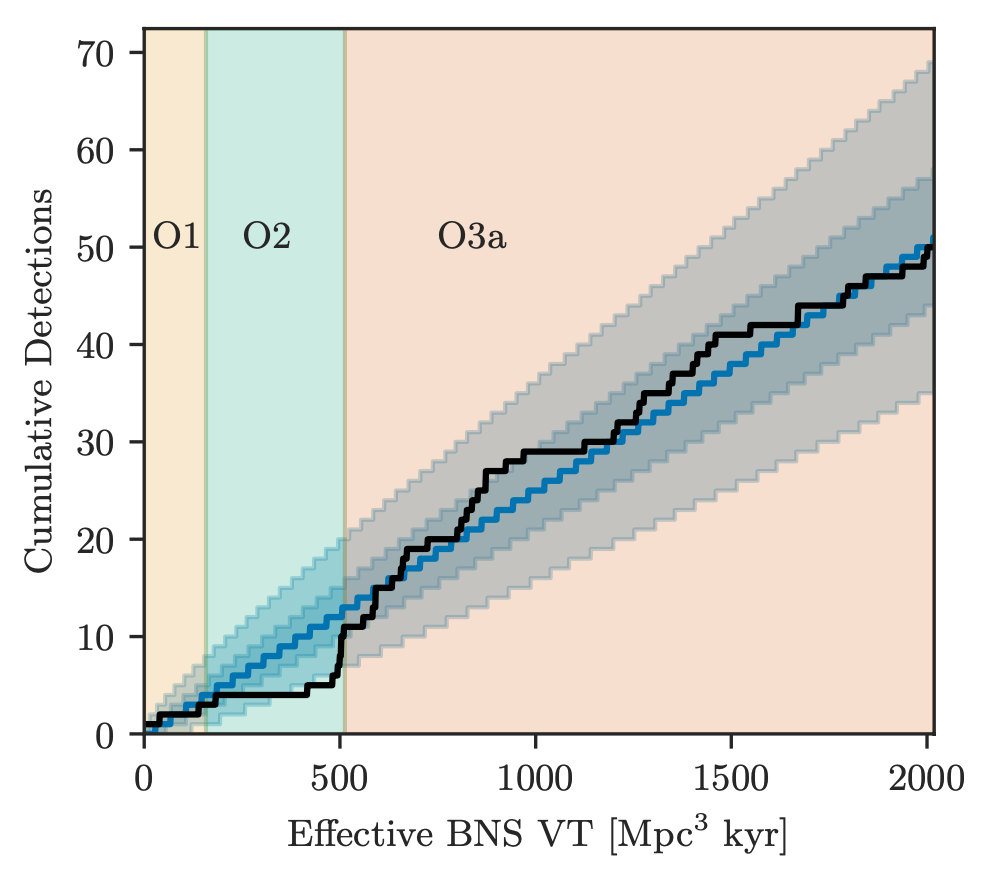
\includegraphics[width=0.6\textwidth]{o3detection}
          \centering
          \caption{The number of compact binary coalescence detections versus the effective volume-time (VT) to which gravitational wave network is sensitive to BNS coalescences. The effective VT is defined as the Euclidean sensitive volume of the second-most sensitive detector in the network at a given time, multiplied by the live time of that network configuration. The Euclidean sensitive volume of each detector is calculated from the BNS inspiral range. The effective BNS VT does not account for differences in sensitivity across the entire population of signals detected or necessary cosmological corrections, but, as shown in this figure, is consistent with the currently observed rate of detections. The coloured bands indicate the three runs, O1, O2, and O3a. The black line is the cumulative number of confident detections of all compact binary coalescences (including black holes and neutron stars) for GWTC-1 and GWTC-2. The blue line, dark blue band, and light blue band are the median, 50\% confidence interval, and 90\% confidence interval of draws from a Poisson fit to the number of detections at the end of O3a \cite{49}.}
          \label{fig:o3detection}
        \end{figure}

        In the remainder of this chapter we will highlight some of the GW observations achieved 
	by the LIGO-Virgo Collaboration and the scientific results connected to them.

\section{The First Observing Run (O1)}
	The first observing run involved the LIGO Hanford Observatory (LHO) and LIGO Livingston Observatory (LLO) detectors, 
	which provided unprecedented sensitivity to GWs
	over a range of frequencies from 30 Hz to several kHz \cite{14}, an interval that  
	covers the frequencies of GWs emitted during 
	the late inspiral, merger, and ringdown of stellar-mass BBHs.

	Two independent matched-filter searches were used to detect GWs from CBC sources: 
	{\ttfamily PyCBC} \cite{109, 110, 111, 112} and {\ttfamily GstLAL} \cite{112, 113, 114}.
	The pipelines identify GW candidates by looking at coincident events 
	found in both LIGO detectors, in a 15\,ms time window 
	that accounts for the inter-site propagation time plus timing uncertainties. 
	Both pipelines used a discrete template bank \cite{42, 114, 115, 117, 118, 119, 120}, 
	targeting binary sources with individual masses from $1{M_\odot}$ to $99{M_\odot}$,
	total mass less than $100{M_\odot}$, and dimensionless non-precessing spins up to 0.99 and 0.05 for BHs and NSs, respectively.

	To assess the candidate significance, they compare the candidate with the noise background, 
	and once an event is confirmed to be a real GW signal, 
	it is removed from the data when estimating the noise background (see Sec.\,\ref{subsec:far}).
	Data affected by short duration artefacts of known origin are identified and removed from the analysis dataset.
	After applying this data quality process, the remaining coincident analysis time in O1 was 48.6\,days. 
	The analyses search only stretches of data longer than a minimum duration, 
	to ensure that the detectors are operating stably and enough data is available to build the background noise distribution.  
	This resulted in 46.1\,days of data for the {\ttfamily PyCBC} analysis and 48.3\,days for the {\ttfamily GstLAL} analysis.

	Three GW events were detected during this run, all three consistent with a BBH source: GW150914, GW151012, and GW151226.
	The binary component masses of all three systems lie 
	within the range expected for stellar-mass BHs. 

\subsection{GW150914: the Birth of Gravitational-Wave Astronomy}
\label{subsec:GW150914}
		\begin{figure}[!t]
                	\label{firstgw}
                	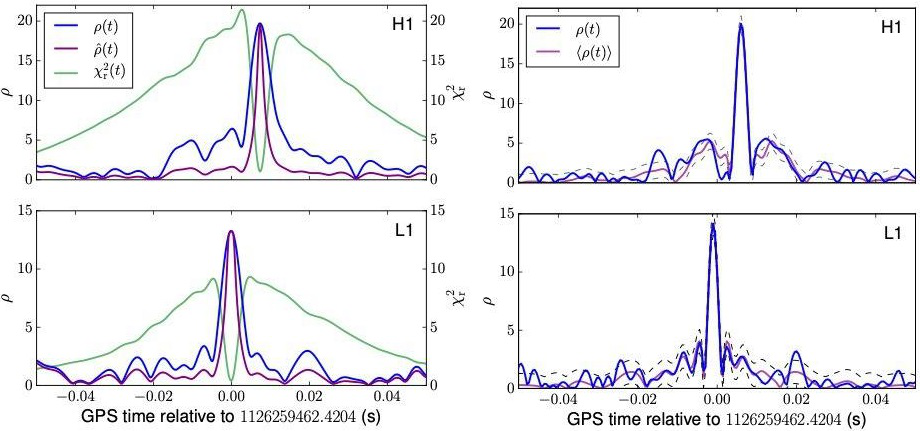
\includegraphics[width=\textwidth]{firstgw}
                	\centering
                	\caption{Left: {\ttfamily PyCBC} matched-filter SNR (blue), re-weighted SNR (purple) and chi-squared (green) versus time for the best-matching template at the time of GW150914. The top and bottom plots refer to the Hanford and Livingston detectors, respectively. Right: Observed matched-filter SNR (blue) and expected matched-filter SNR (purple) versus time for the best-matching template at the time of GW150914, as reported by the {\ttfamily GstLAL} analysis. The expected matched-filter SNR is based on the autocorrelation of the best-matching template. The dashed black lines indicate 1-$\sigma$ deviations expected in Gaussian noise. \cite{21}} 
                	\label{fig:firstgw}
                \end{figure}

	The era of GW astronomy began with the detection of the coalescence of two stellar-mass BHs
	on September 14, 2015 at 09:50:45 UTC.  
	The signal GW150914 was detected with a matched-filter network SNR of 23.7 \cite{21}. 
	Both {\ttfamily PyCBC} and {\ttfamily GstLAL} identified GW150914 as the most significant event in O1 and the probability that 
	it was due to a random coincidence of detector noise is extremely small: 
	both pipelines found no background events with significance 
	equal to or greater than GW150914.  
	Therefore only an upper limit on the FAR of GW150914 was determined: $6.0 \times 10^{-7}\,$yr$^{-1}$. 
	This corresponds to a $p$-value of $7.5\times10^{-8}$, or a Gaussian-equivalent significance of $5.3\sigma$.  
	In Fig.\,\ref{fig:firstgw}, taken from \cite{21}, we show a snapshot of the {\ttfamily PyCBC} (left) 
	and {\ttfamily GstLAL} (right) analyses around the time of GW150914.  
	The SNR time-series (blue) and re-weighted SNR (purple) time-series
	obtained with the best-matching template peak at time of GW150914, 	
	while the normalised chi-squared (green) dips suddenly; 
	this behaviour is observed at both detectors (Handford top, and Livingston bottom).  
	A similar behaviour holds for the {\ttfamily GstLAL} data that shows the SNR (blue) and expected SNR (purple) time-series
	for the same best-matching template.  
	The two time-series vary consistently with one another, 
	within the 1-$\sigma$ deviations reported by the black dashed line.

\subsubsection{Masses}
	The physical parameters of the source of GW150914 were inferred using two waveform models, 
	a non-precessing effective-one-body waveform model (EOBNR) \cite{103, 104} 
	and a precessing spin model (IMRPhenom) \cite{105, 106, 107}. 
	Results from the two waveforms are consistent, and match the expectations 
	for a coherent signal of astrophysical origin in both detectors. 
	The total mass of GW150914 was found to be $M^{\rm source} = 65.3^{+4.1}_{-3.4}M_\odot$, 
	with individual masses of $36^{+5}_{-4}M_\odot$ and $29^{+4}_{-4}M_\odot$ \cite{21,41,51}.  
	This makes the source compatible with a near-equal mass BBH system.
	Following the inspiral, a BBH merges to form a BH remnant; in the case of this signal, 
	the mass of the remnant was $M^{\rm source}_f = 62.3^{+3.7}_{-3.1}M_\odot$.
	The $\sim 3M_\odot$ of difference between $M^{\rm source}$ and $M^{\rm source}_f$ are radiated away in GWs.  
	While predominantly determined by the total mass, 
	the radiated energy also depends upon the mass ratio and component spins.

\subsubsection{Spins}
	The results obtained for GW150914 are consistent with expectations for moderately spinning BHs \cite{101, 102}. 
	For equal mass binaries, both components of the spin, 
	parallel and orthogonal to the orbital angular momentum, 
	play a role in the dynamics, but, as the mass ratio tends to zero, 
	the effects of the secondary spin become negligible.
	The spin of the remnant BH, as its mass, is calculated using fitting formulas 
	calibrated against numerical relativity simulations.  
	It was inferred to be $0.69^{+0.05}_{-0.04}$, as expected for near equal-mass BBH mergers 
	for which the final spin is dominated by the orbital angular momentum of the binary at merger \cite{99, 100}.

\subsubsection{Distance, Inclination, and Sky Location}
	The signal amplitude is inversely proportional to the luminosity distance to the source: 
	GW150914 has an estimated distance of $D_L = 440^{+150}_{-170}\,$Mpc (redshift $z=0.09^{+0.03}_{-0.03}$). 

	The significant fractional uncertainty for the distance is due to the degeneracy 
	between the distance and the binary inclination with respect to the observer, which both impact the signal amplitude \cite{96, 97, 98}.
	The configurations for which the orientation of the binary produces the greatest GW amplitude 
	are either face-on or face-off (angular momentum pointed parallel or antiparallel to the line of sight). 
	The inclination could potentially be better constrained in a precessing system \cite{94, 95}. 
	For GW150914, the data provides a greater posterior support for the source being face-off \cite{93}.

	Sky localisation from a GW detector network is primarily determined by the measured delay in the signal arrival times at the sites, 
	with additional information coming from the signal amplitude and phase \cite{91,12}. 
	The arrival time at Hanford relative to Livingstone was $\Delta t_{HL} = 7.0^{+0.02}_{-0.02}$\,s.
	The 90\% credible region for the sky location of the source of GW150914 had an area of $230\,$deg$^2$.
	The sky area scales inversely with the square of the SNR \cite{89,90}, 
	and this trend is followed as this event had the smallest sky localisation and 
	highest SNR amongst the events detected during O1.

\subsubsection{Astrophysical Implications}
	This GW discovery provides the first robust confirmation of several theoretical predictions, beyond the existence of GWs:
	heavy BHs exist, BBHs form in nature, and BBHs merge within the age of the Universe at a detectable rate. 
	However, it was impossible to determine the formation channel for this event. 
	Possible BBH formation channels include dynamical formation in a dense stellar environment \cite{84, 88} 
	possibly assisted by gas drag in galactic nuclear disks \cite{82, 83}, or isolated binary evolution, 
	either the classical variant via a common-envelope phase \cite{76, 77, 78, 79, 80, 81}, 
	potentially from population III binaries \cite{74, 75}, or chemically homogeneous evolution 
	in close tidally locked binaries \cite{72, 73}. 
	All of these channels have been shown to be consistent with the GW150914 discovery \cite{63, 64, 65, 66, 67, 68, 69, 70}. 

        \begin{figure}[!t]
          \label{o1}
          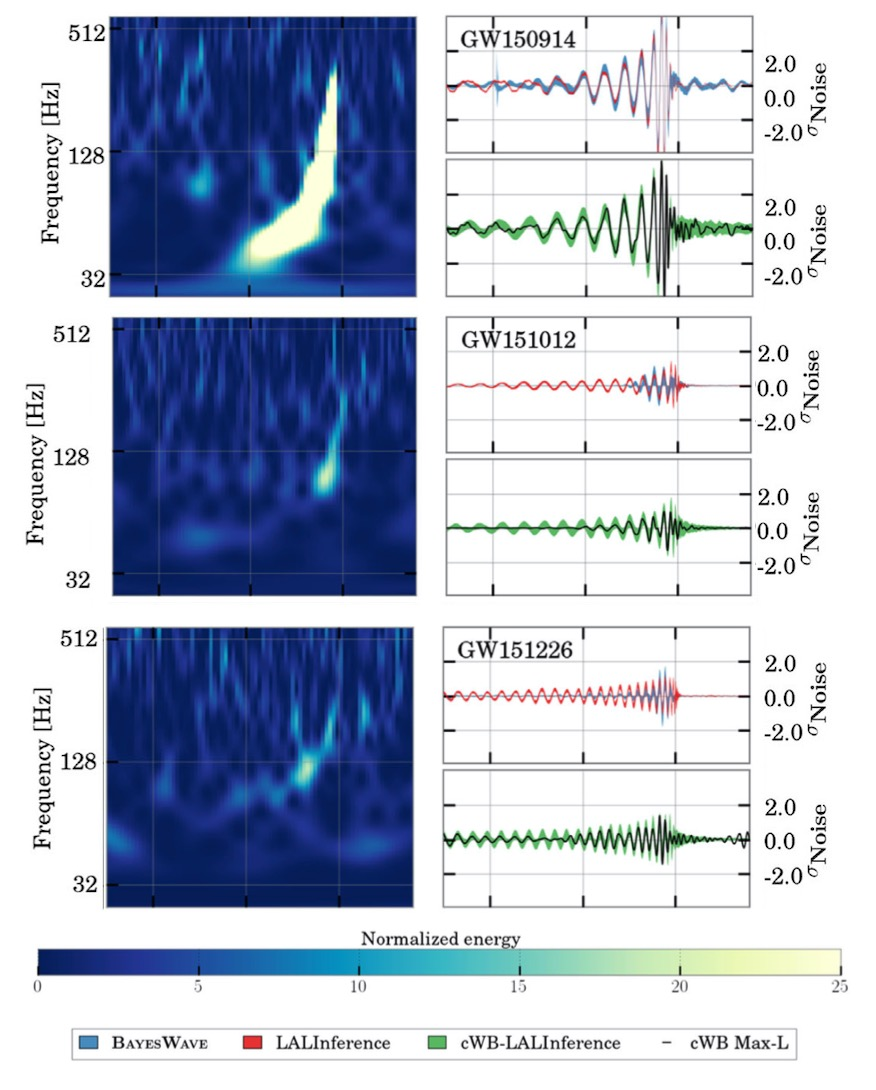
\includegraphics[scale=0.4]{o1}
          \centering
          \caption{Time-frequency maps and reconstructed signal waveforms for the three O1 BBH events. Each row refers to a single event.  The three panels in a row show whitened data from the LIGO detector where the higher SNR was recorded. The panel on the left is a normalised time-frequency power map of the GW strain.  The two panels on the right show time-domain reconstructions of the whitened signal, in units of the standard deviation of the noise. The upper panel shows the 90\% credible intervals from the posterior probability density functions of the waveform time-series inferred by a Bayesian pipeline that used the PhenomP waveform templates ({\ttfamily LALInference}, red band) and by a pipeline that used wavelet reconstruction ({\ttfamily BayesWave}, blue band).  The lower panel shows the maximum likelihood point estimate from the {\ttfamily coherent WaveBurst} unmodelled search (solid lines), along with a 90\% confidence interval (green band) derived from the {\ttfamily coherent WaveBurst} analyses of simulated waveforms generated starting from the {\ttfamily LALInference} posterior and injected into data near each event. \cite{13}}
          \label{fig:o1}
        \end{figure}


\subsection{GW151012 and GW151226}
	Two more GW signals were detected during O1, and both were consistent with a BBH source: 
	GW151012 and GW151226.  
	A summary of all three observations is provided in Fig.\,\ref{fig:o1} \cite{13}.  
	This shows the time-frequency maps and reconstructed waveforms for all three O1 events.

	GW151012 is the third most significant GW event from O1.  
	It was first referred to as LVT151012, where LVT stands for LIGO-Virgo Transient: 
	this was due to the fact that it was originally detected with a low statistical significance of $1.7\sigma$, 
	corresponding to a FAR of one in 2.7 years.  
	The trigger was later reanalysed with improved O2 versions of the pipelines and its significance was increased: 
	the signal now meets the criteria of a confident detection of a BBH merger, 
	and was therefore re-labeled as GW151012.  
	The final values of the network SNR for this signal are 9.5 and 10.0 
	for the {\ttfamily PyCBC} and {\ttfamily GstLAL} pipelines, respectively \cite{13}.

	GW151226 was the second observation of a coincident GW signal to be announced. 
	Its combined matched-filter SNR was 13. 
	The signal was identified as the second most significant event by both the {\ttfamily PyCBC} and {\ttfamily GstLAL} analyses.
	GW151226 was more significant than all O1 background events in the {\ttfamily PyCBC} analysis, 
	after having removed any background events associated with GW150914 from the distribution.
	Its FAR has an upper limit of $6.0 \times 10^{-7} yr^{-1}$, which
        corresponds to a $p$-value of $< 7.5 \times 10^{-8}$, or a Gaussian-equivalent significance of at least $5.3\sigma$. 
	In the {\ttfamily GstLAL} analysis, the background extends past the observed log-likelihood of GW151226, 
	and the event is recovered with a FAR of 1 per 44000 years, which corresponds to a $p$-value of $3.5\times 10^{-6}$ and a significance of $4.5\sigma$.

	GW151226 persisted in the LIGO frequency band for approximately 1\,s, 
	increasing in frequency and amplitude over about 55 cycles from 35 to 450\,Hz. 
	This differs from the more massive GW150914 binary for which only the last 10 cycles of the inspiral where observable.  
	Since the chirp mass is the physical parameter which controls the binary evolution during the early inspiral, 
	the longer signal has an immediate effect on the precision 
	with which the chirp mass \cite{98,126} was recovered with respect to the case of GW150914.
	While GW151226 has an inferred chirp mass $\mathcal{M}=8.9\pm 0.3 M_\odot$,
	GW150914 has $\mathcal{M}=27.6\pm 2  M_\odot$.

	The source of GW151226 was an unequal-mass system with two stellar-mass BHs 
	with a source-frame masses of $m_1 = 13.7^{+8.8}_{-3.2}M_\odot$ 
	and secondary mass $m_2 = 7.7^{+2.2}_{-2.5}M_\odot$ \cite{13}. 
	The inferred BH masses are within the range of dynamically measured masses 
	of BHs found in X-ray binaries \cite{128, 129, 130, 132}, 
	unlike the high masses of GW150914 which had never been observed before. 
	Finally, the two LIGO detectors are nearly co-aligned and the source of GW151226 
	is likely to be located close to the maxima of the directional responses of both detectors \cite{28}. 
	Consequently, it is difficult to extract the polarisation content, and therefore the orientation of the orbital plane. 
	As a result, the luminosity distance is only weakly constrained to be $D_L = 450^{+180}_{-190}Mpc$, 
	which is comparable to the one of GW150914 and corresponds to a redshift of $0.09^{+0.04}_{-0.04}$.


\section{The Second Observing Run (O2)}
	Between O1 and O2 run the sensitivity of both LIGO instruments was improved and 
	at LLO further improvements were made during O2. 
	As a result, the LLO BNS range --- i.e., the distance, averaged over sky position and inclination, 
	up to which a binary made by two $1.4M_\odot$ NSs is detectable --- 
	increased from about 60\,Mpc to 80\,Mpc at the beginning of O2.  
	This was later increased by another $\sim 20\%$.
 	Despite its lower BNS range ($\sim 25\,$Mpc) Virgo provided a fundamental contribution 
	in determining the source localisation and orientation \cite{56}, 
	as well as in boosting the significance of the events. 
	This was of paramount importance in kick-starting multi messenger astronomy with GWs.
	In addition to the instrument upgrades, developments were also carried out on
	the search algorithms.
 
	Of the eight GW signals detected during O2 
	(GW170104, GW170608, GW170729, GW170809, GW170814, GW170817, GW170818 and GW170823), 
	the five August events were localised by the three detector LHO, LLO and Virgo (HLV) network.  
	Additionally, GW170104, GW170814, GW170608, and GW170817 where published, 
	in that order, as single events \cite{60,61,62,138}.   
	In order to quantify the FAR with an accuracy that enabled the claim of confident detections, 
	the O2 data was divided into periods of 5 days of two-detector cumulative coincident observing time.
	This time, the searches targeted  detector-frame total masses from $2M_\odot$ to $500 M_\odot$, 
	whereas the spin target space remained unchanged.
	Since GW151226 is a low mass binary, the chirp  mass is well measured $8.9^{+0.3}_{-0.3} M_\odot$,
	while for the higher mass system GW150914 is $28^{+2}_{-2}M_\odot$.

\subsection{GW170104: a 50-Solar-Mass Binary Black Hole Coalescence}
	The observation of GW170104 was made by the LIGO detectors, 
	with a network SNR of 13 and a FAR of less than 1 in 70,000 years.
	At the detection statistic value of GW170104, the background rate in both matched filter 
	analyses is dwarfed by the signal rate, 
	yielding a probality of astrophysical origin greater than $1 - (3 \times 10^{-5})$ \cite{60}.

	The source of GW170104 is a BBH system with total mass of $\sim 50M_\odot$.  	
	The inferred component masses are $31.2^{+8.4}_{-6.0}M_\odot$ and $19.4^{+5.3} _{-5.9}M_\odot$.
	The BH spins are best constrained through measurement of the effective inspiral spin parameter, $\chi_{\rm eff}$, 
	a mass-weighted combination of the spin components perpendicular to the orbital plane; 
	the credible interval found was $\chi_{\rm eff} = −0.12^{+0.21}_{−0.30}$. 
	This result implies that the BH spins show a preference for being 
	anti-aligned with the orbital angular momentum, but the zero spin possibility is not excluded. 
	This is distinct from the case for GW151226, which had a strong preference 
	for spins with positive projections along the orbital angular momentum \cite{58}.
	Finally, the source luminosity distance is $880^{+450}_{−390} Mpc$ corresponding to a redshift of $z = 0.18^{+0.08}_{−0.07}$. 

	The high source mass values suggest formation in a sub-solar metallicity environment \cite{134}, 
	which weakens the stellar winds that cause mass loss during the lifetime of the progenitor stars.
	The inferred merger rate agrees with previous calculations \cite{59, 137}, and could potentially be explained 	
	by BBHs forming through isolated binary evolution or dynamical interactions in dense stellar clusters \cite{134}. 

\subsection{GW170608}
	GW170608 was first identified as a loud (SNR $\sim9$) event in LLO data,
	via low-latency templated searches \cite{138}.	
	The morphology of the LLO event is consistent with a CBC signal, 
	but a noise origin could not be ruled out using LLO data alone. 
	Consequently, LHO data were investigated and were determined to be stable 
	at frequencies above 30Hz, which was established as the starting frequency 
	to look into a segment of LHO data around the event time.
	{\ttfamily PyCBC} and {\ttfamily GstLAL} then identified GW170608 with a network SNR of 13,
	and a FAR of less than 1 in 3,000 years and 1 in 160,000 years, respectively.

	The binary source of GW170608 consisted of two compact objects with source-frame component masses 
	$12^{+7}_{-2}M_\odot$ and $7^{+2}_{-2}M_\odot$.  
	Since NSs are expected to have masses below $\sim 4M_\odot$ \cite{141},
	both objects are most likely BHs. 
	The $\chi_{\rm eff}$ inferred from this event is $0.07^{+0.23}_{−0.09}$,
	disfavouring large, anti-aligned spins on both BH.
        Finally, GW170608 was localised at a luminosity distance of $D_L = 340^{+140}_{−140}Mpc$, 
	and within a sky area of $\sim 520\,$deg$^2$, determined largely by the signal's measured arrival time at LLO $\sim 7$\,ms later than at LHO.
 
	The inferred component masses of GW170608 are consistent with 
	dynamically-measured masses of BHs found in low-mass X-ray binaries.
	The low masses involved imply that this time a high-metallicity progenitor environment is possible, 
	as this causes significant mass losses from the progenitor stars via strong stellar winds.
	However, formation at lower metallicity with comparatively lower mass progenitors is not excluded.

\subsection{GW170814: the First Three-Detector Network Observation}	
	On August 14, 2017, a GW signal coming from the merger of two stellar mass BHs 
	was observed for the first time by a three detector network, comprised of the Virgo and two LIGO detectors. 
	GW170814 was first identified with high confidence by two independent 
	low-latency matched-filter pipelines \cite{111,112,114,146},
	with a Hanford-Livingston network SNR of 15 and a three-detector network SNR of 18 \cite{114,150,151}.
	The improvement in significance achieved by including Virgo data in the analysis is particularly evident 
	for this event: when data from all thee detectors is used, 
	the FAR of the event is $< 1$ in 5,900 years, while the LIGO-only FAR is approximately 1 in 300 years.

	The component masses of the source inferred through a coherent Bayesian analysis \cite{93, 152} 
	of offline noise-subtracted data for the LIGO and Virgo detectors 
        are $30.5^{+5.7}_{-3.0}M_\odot$ and $25.3^{+2.8}_{-4.2}M_\odot$.
	For events detected by the two LIGO instruments alone, the localisation 
	was often limited to roughly annular regions by the baseline formed by the two LIGO detectors,
	spanning hundreds to about a thousand square degrees at the 90\% credible level \cite{89,155,156}. 
	The inclusion of Virgo contributes with additional independent baselines, 
	which for GW170814 and similar events can reduce the positional uncertainty by an order of magnitude or more \cite{155}. 
	For an initial rapid localisation performed with LHO and LLO data, 
	the 90\% credible area on the sky was $1160\,$deg$^2$: the inclusion of Virgo shrunk this down to $100\,$deg$^2$.
	Incorporating Virgo data also reduces the uncertainty on luminosity distance, 
	which goes from $570^{+300}_{-200}\,$Mpc (two-detector rapid localisation) to $540^{+130}_{-210}\,$Mpc (full network).

	Since the two LIGO instruments have similar orientations, 
	the information about polarisation is minimal when the LIGO instruments alone.  
	Virgo data allowed to investigate GW polarisations for the first time, by geometrically 
	projecting the wave amplitude onto the three detectors.
	Generic metric theories predict that any combination of tensor, vector, or scalar 
	polarisations \cite{85} can characterise metric perturbations.
	So far, some evidence that GWs are described by the tensor (spin-2) metric perturbations 
	of general relativity has been obtained from measurements of the orbital decay rate of binary pulsars \cite{135,140}, 
	and from the GW phase evolution of BBH mergers observed by LIGO, in the framework of parametrised models \cite{14,52,60}. 
	The results of the analysis of GW170814 with Virgo data show that the data strongly favour
	pure the tensor polarisations of general relativity, over pure scalar or pure vector polarisations.

        \begin{figure}[!t]
          \label{o2}
          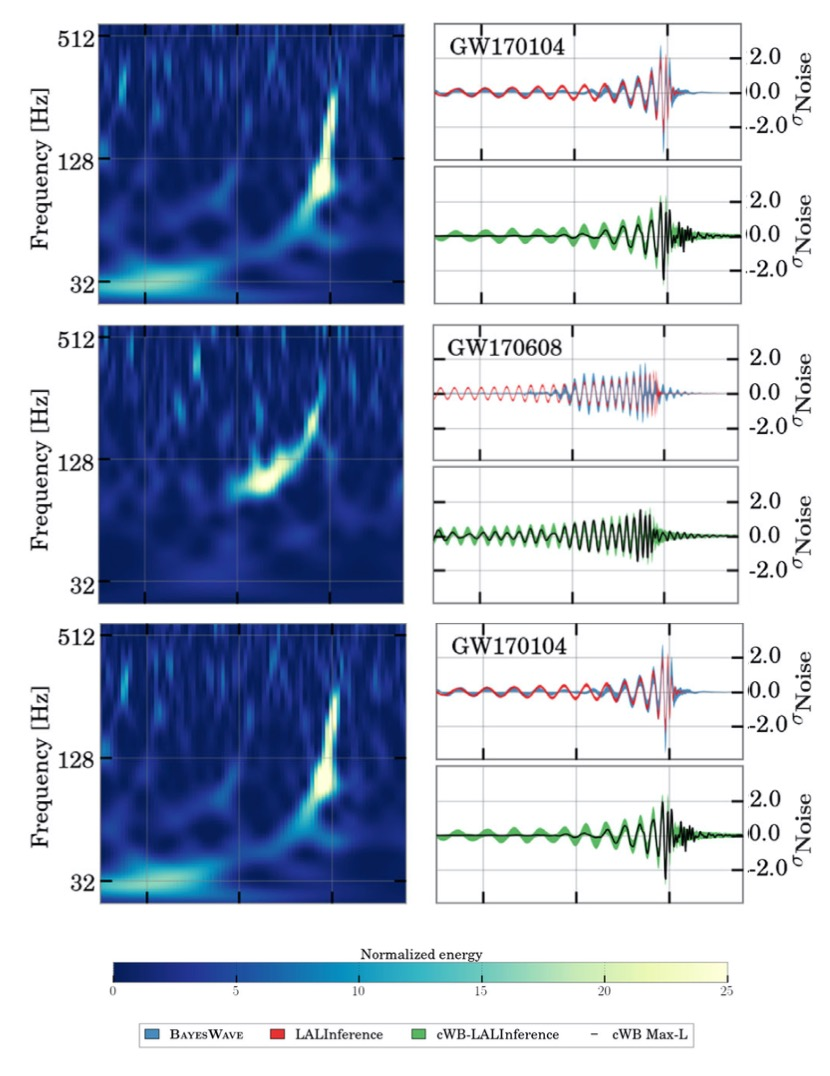
\includegraphics[scale=0.45]{o2}
          \centering
          \caption{Same as Fig.\,\ref{fig:o1} but for the O2 events: GW170104, GW170608 and GW170814.}
          \label{fig:o2}
        \end{figure}

\subsection{GW170817: the Birth of Multimessenger Astronomy}
\label{subsec:GW170817}
	On 17 August 2017 the first GW signal compatible with a BNS source 
	was detected by the LIGO-Virgo Collaboration.  
	The GW170817 candidate was first registered in low latency \cite{112,114}
	as a single-detector trigger in LHO data. 
	An offline re-analysis \cite{28,111} of data from the whole LIGO-Virgo network 
	confirmed the presence of a significant coincident signal with a combined SNR of 32.4.
	The offline analysis then identified the FAR of GW170817 to be less than 1 in 80,000 years \cite{61}. 
	The source was localised \cite{59,152} in a region of $28\,$deg$^2$ at a distance of $40^{+8}_{-14}$ Mpc, 
	consistently with the early estimates disseminated through GCN Circulars \cite{55,60}.
	The inspiral stage of the binary coalescence dominates 
	the portion of GW170817 in the detector sensitivity bands, 
	and as a consequence, the chirp mass, 
	which drives the frequency evolution of gravitational radiation at the leading order, 
	is the best constrained parameter with a value of $1.188^{+0.004}_{-0.002}M_\odot$.
	The measured component masses are in the range $0.86$--$2.26M_\odot$
	consistent with a compact binary with two NSs.

        In of itself this observation already constitutes a remarkable result, 
	but more historical results poured in that day and in the following months.  
	$\sim1.74$\,s after the trigger time of GW170817, the {\it Fermi}/GBM and INTEGRAL SPI-ACS instruments 
	recorded GRB 170817A \cite{147} which was shown to be unambiguously associated 
	with the source of GW170817 \cite{55}.  
	This was the first confident joint GW and electromagnetic observation in history (see Fig.\,\ref{fig:gw-grb}).
	Standard follow-up analyses \cite{108,110} of the {\it Fermi}/GBM trigger 
	determined the burst duration to be $T_{90} = (2.0 \pm 0.5)\,$s,
	therefore GRB 170817A was classified as a short GRB, with 3:1 odds over being a long GRB.
        The classification is further supported by incorporating 
	the hardness ratio of the burst and comparing it to the {\it Fermi}/GBM catalog \cite{110}.  
	The unambiguous association of GW170818 and short GRB 170817A confirmed that BNSs 
	can be the progenitors of short GRBs, a question that had remained open for decades in high-energy astrophysics.

        Having received notice of the observation of short GRB 170817A by {\it Fermi}, 
	the LIGO-Virgo Collaboration ran two offline targeted {\it coherent} searches on its data, 
	as it does for all {\it Fermi} and {\it Swift} GRB observations.  
	The first targeted search ({\ttfamily PyGRB} \cite{111,116}
	looks for sub-threshold GW signals in the data by searching for BNS and NS–BH binary merger signals 
	compatible with the time and sky-location of short GRBs.  
	This search is carried out in a $[-5, +1]\,$s window around the GRB trigger time \cite{55}. 
	This search recovered GW170817, as expected, with a $p$-value of $<9.4\time 10^{-6}(>4.2\sigma)$: 
	this significance estimate is limited by computational resources used to estimate the noise background. 
	The second coherent search does not assume any particular GW morphology or GRB model 
	\cite{43,55,161} and it allows for a $[-600, +60]\,$s search window,
	in order to address potentially higher time-of-arrival separations 
	that may arise for long GRB triggers.
	This unmodelled search also recovered GW170817, with a $p$-value of $1.3\times 10^{-5} (4.2\sigma)$.

	The observation with excellent localisation of GW170817 triggered 
	a huge electromagnetic follow-up campaign \cite{63} 
	which produced observations across the whole electromagnetic spectrum.
	This captured an infrared transient (kilonova), 
	which allowed for the identification of the host galaxy of the source 
	and is associated with the aftermath of the BNS merger.
	Delayed X-ray and radio counterparts that provide information 
	on the environment of the binary where also registered.
        
        \begin{figure}[!t]
          \label{gw-grb}
          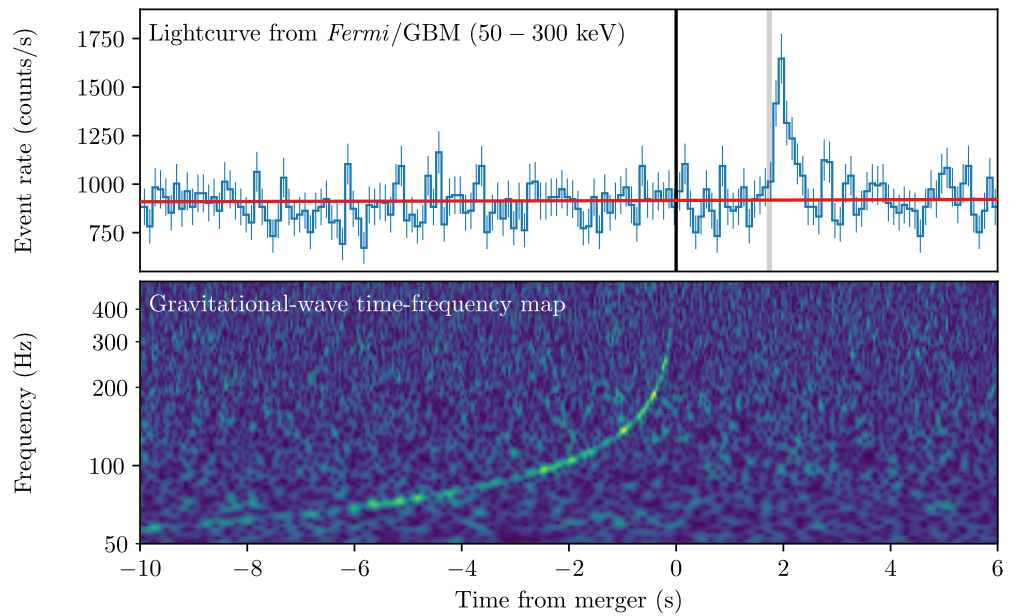
\includegraphics[width=\textwidth]{gw-grb}
          \centering
          \caption{Joint, multi-messenger detection of GW170817 and GRB 170817A. Top: the GBM lightcurve in the 50--300\,keV energy range. The background estimate from \cite{110} is overlaid in red. Bottom: the time-frequency map of GW170817  obtained by coherently combining LHO and LLO data. All times here are relative to the GW170817 trigger time. \cite{55}}
          \label{fig:gw-grb}
        \end{figure}


\section{The Third Observing Run (O3)}
	Between O2 and O3, several improvements were made to increase the detector sensitivities.  For the LIGO detectors, 
	the input laser power was increased, a squeezed vacuum source 
	at the interferometer output was added and noise arising from scattered light was mitigated.  
	Additionally, end test-mass optics with lower-loss coatings, 
	along with new reaction masses, 
	were installed in each interferometer \cite{53}. 
	The BNS inspiral range reached $102$--$111\,$Mpc for LHO and $125$--$140\,$Mpc for LLO during the first part of O3.
	Virgo doubled its sensitivity compared to O2, 
	thanks to a series of improvements: 
	fused silica fibers were installed as a replacement of the steel test-mass suspensions, 
	technical noises were reduced, the input laser power was increased 
	and a squeezed vacuum source was installed. 
	This brought the Virgo BNS inspiral range to $43$-–$50\,$Mpc over the first three months of O3, 
	as shown in Fig.\,\ref{fig:o3bnsrange}. 
	These improvements successfully impacted the detection rate (Fig.\,\ref{fig:o3detection}).  
        During the first half of this observing run,
        thirty-nine events passed the 2.0 yr$^{-1}$ candidate threshold.
        Among these candidate events, four have already been published as special events:                            
        O3a uncovered the largest and smallest BBH to date, ranging from 150 times the size of the sun (GW190521) to just 3 times larger (GW190425).
 	The first BBH confidently formed from highly asymmetrical BHs (GW190412) was also detected, 
	as well as a binary, whose smallest component is an unidentified massive compact object \cite{49}.
        
        \begin{figure}[!t]
          \label{o3bnsrange}
          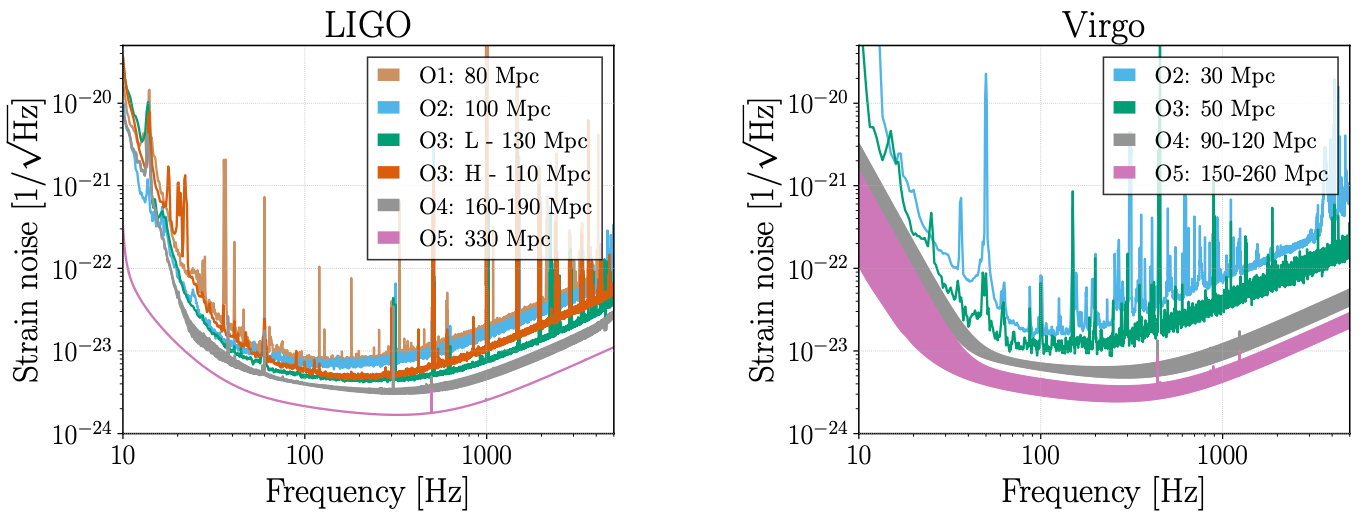
\includegraphics[width=\textwidth]{o3bnsrange}
          \centering
          \caption{Advanced LIGO (top left), Advance Virgo (top right) target strain sensitivities as a function of frequency. The quoted range is for a $1.4M_\odot + 1.4M_\odot$ BNS merger.  The BNS range (in Mpc) achieved in past observing runs and anticipated for future runs is shown.  The O1 LIGO curve is taken from the LHO, while the O2 one comes from LLO; in both cases they refer to the interferometer with better performance for the observing run in question. The O3 curves reflect recent performance. For future runs the anticipated ranges are shown as bands reflecting the uncertainty in the impact of improvements and upgrades to the overall sensitivity. \cite{53}}
          \label{fig:o3bnsrange}
        \end{figure}

\subsection{GW190412: a Binary-Black-Hole with Asymmetric Masses}
\label{subsec:GW1901412}
	GW190412 is a loud event detected with by the LIGO-Virgo three detector network 
	with network SNR of 19 and a FAR of 1 in 30,000\,yrs.
	The peculiarity of this event is the asymmetry in the binary component masses:
	one is a $\sim 8M_\odot$ BH, while its companion has a mass of $\sim 30M_\odot$.
	While the individual masses of the BBH were consistent with those of preious GW events,
	the mass ratio is unlike any of the other BH mergers detected before. 
	This allows to observe a fundamental property of GWs.

	In general relativity, gravitational radiation
	is observed as a combination of two polarisations, weighted with the detector response functions, see Eq.\,(\ref{beampattern}). 
	This quantity can be expressed also as $h = h_{+}-ih_{\times}$ and expanded into multipole moments 
	using spherical polar coordinates defined in a source centered frame \cite{133}
        \begin{equation}
          h_{+}-ih_{\times} = \sum_{l \geq 2} \sum_{-l \leq m \leq l} {{h_{lm}(t, \boldsymbol{\lambda})} \over {D_L}} _{-2} Y_{lm}(\theta, \phi)
        \end{equation}
	The radiative multipoles, $h_{lm}$, depend on the source properties, while the source geometry 
	depends on mass ratio and is most prominently manifested in the relative contribution 
	of multipoles with odd or even azimuthal index, $m$.
	For an exactly equal mass binary with non-spinning components, only multipoles with even $m$ 
	respect orbital symmetry and so are present in the radiation \cite{158}, resulting in the quadrupole, $h_{22}$, 
	being the most dominant, followed by other multipoles with even $m$. 
	Otherwise, for sufficiently unequal mass ratios, the $l = m = 3$ and subsequent 
	multipoles with $l = m$ gain increasing importance \cite{158, 159, 160}.
	GWs of higher harmonics had not been observed until GW190412:
	these higher multipoles makes a significant, measurable contribution to the observed data as shown in \cite{133}.

	As a result of the richer detectable multipole content, 
	the orientation of the binary is more accurately determined and 
	tighter bounds are obtained on intrinsic source parameters, 
	such as the mass ratio and primary spin magnitude, 
	which constitutes the tightest constraint on the individual spin magnitude of a BH obtained with GWs so far. 
	Even though the $\chi_{\rm eff}$ is found to be positive, 
	large in-plane spin components are absent, 
	indicating that the system is slightly precessing.
	The degeneracy between luminosity distance and inclination angle that is typical 
	in the results obtained when higher multipoles are suppressed is broken when higher multipoles are visible, 
	resulting in more precise measurements of these parameters.

	The new observation also provides new insight into the BBH merger rate, 
	showing clearly that unequal-mass systems are less likely, but still expected to form in the universe. \cite{133}

        \begin{figure}[!t]
          \label{asymmetric}
          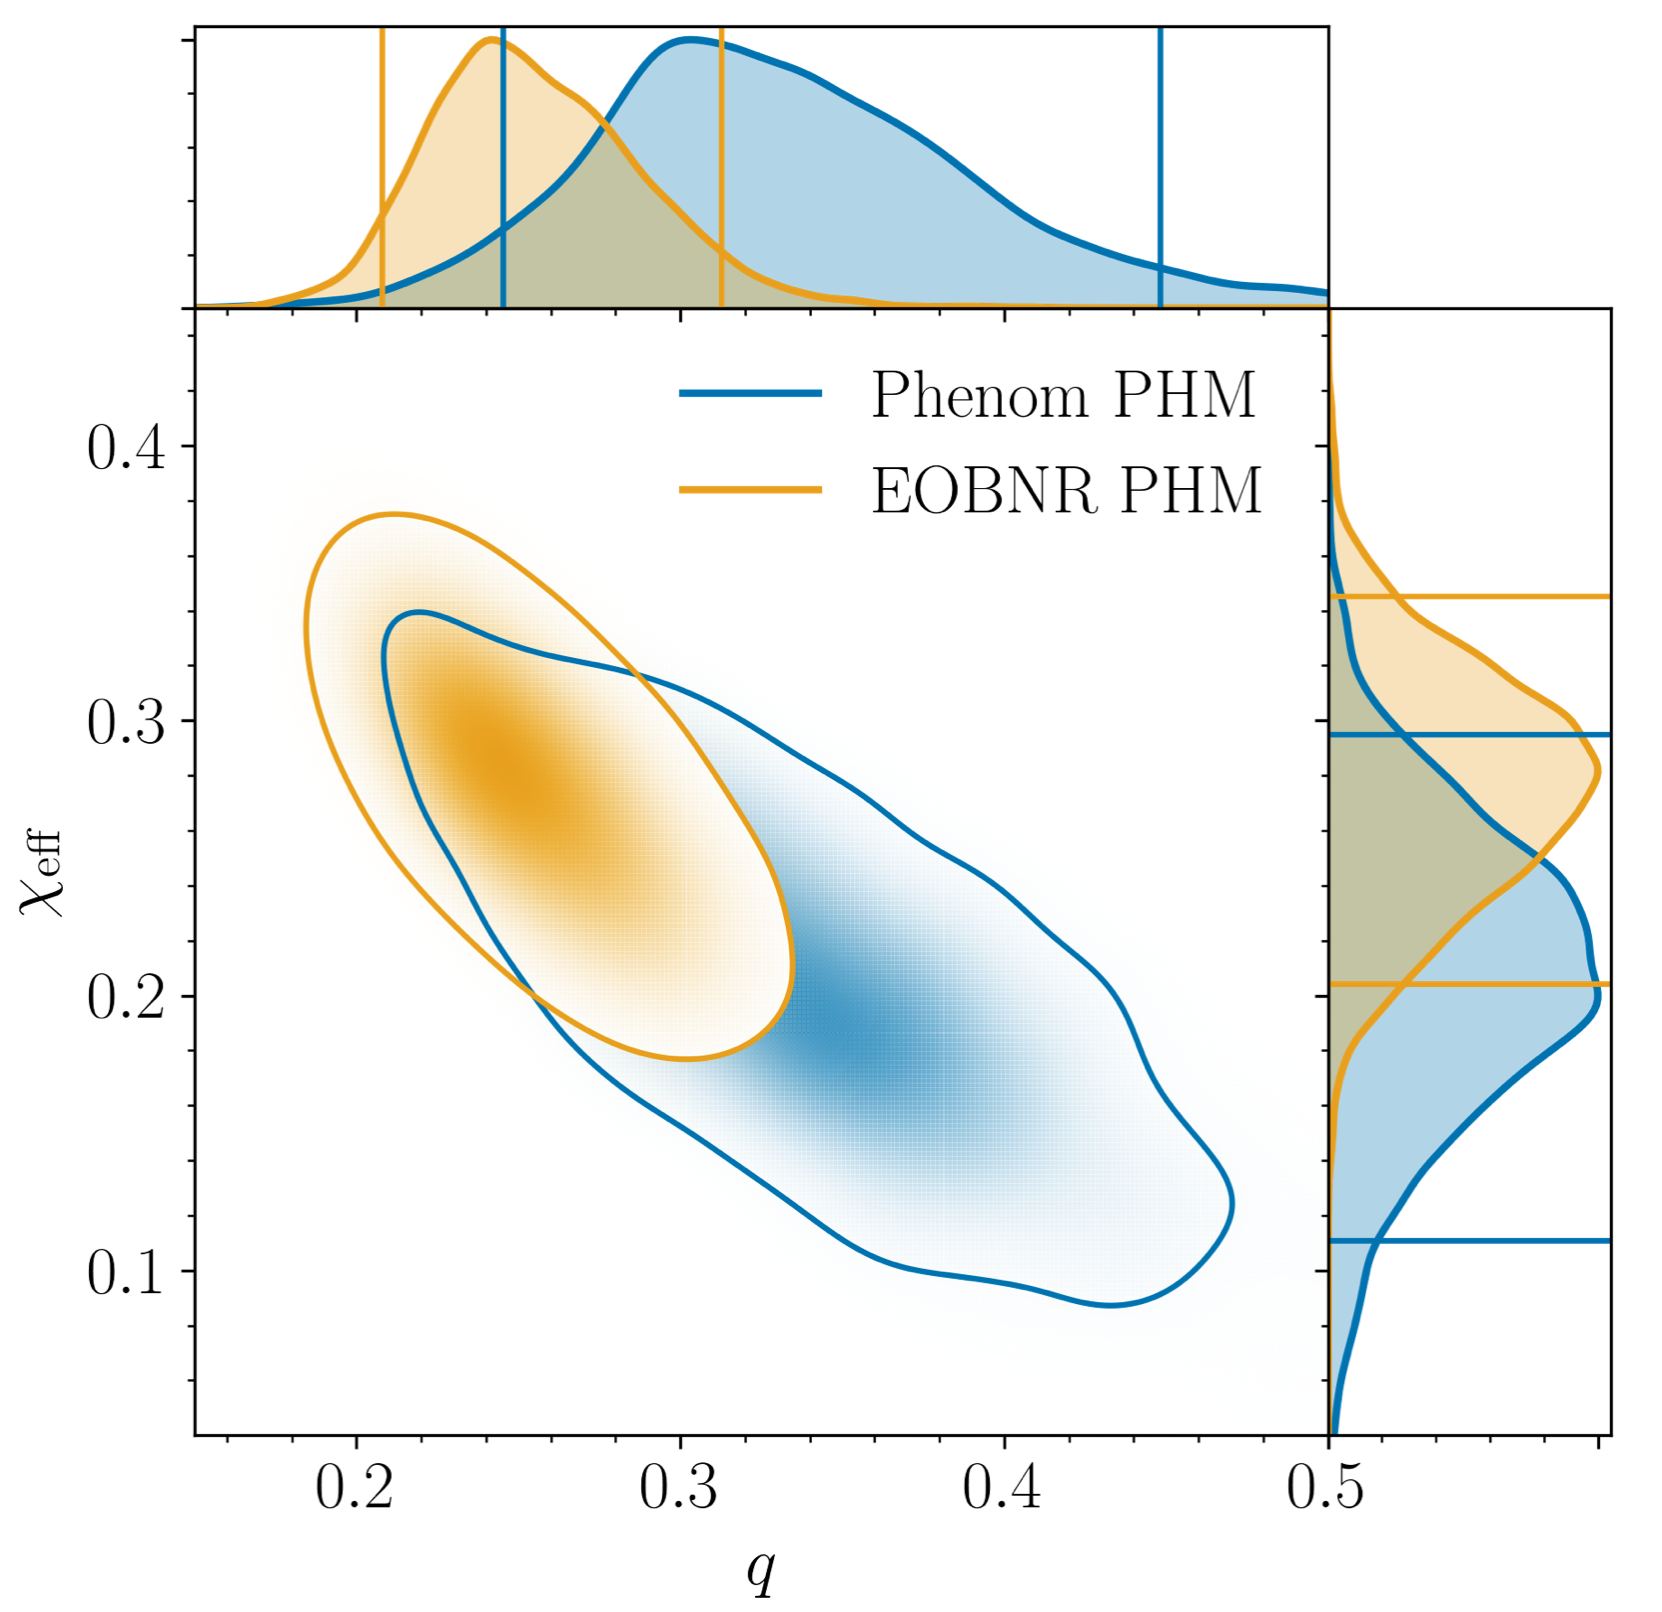
\includegraphics[width=0.6\textwidth]{asymmetric}
          \centering
          \caption{The inferred mass ratio $q$ and effective spin $\chi_{\rm eff}$ of GW190412. The distributions reported in orange and blue are obtained with two distinct waveform models. \cite{133}} 
          \label{fig:asymmetric}
        \end{figure}

\subsection{GW190425: a Compact Binary Coalescence with Total Mass of About $3.4$ Solar Masses}
\label{subsec:GW190425}

	GW190425, observed by LLO, is the second GW event
	consistent with the inspiral of a BNS system.
	This event was detected in real time processing, with an SNR of 12.9 in LLO; 
	Virgo was operating at the time of the event, but observed the event with an SNR of 2.5, 
	which is below the threshold of 4 at which searches consider triggers for significance estimation. 
	The difference in SNR between LLO and Virgo is consistent with the difference 
	in the sensitivities of the two detectors, considering that LLO had 
	a BNS inspiral range of $\sim 135\,$Mpc, while for Virgo it was $\sim 48\,$Mpc.

	The single detector observation has a couple of consequences. 
	One is that the localisation area is the sky is so large
	that it constitutes a significant challenge for follow-up searches for electromagnetic counterparts. 
	The absence of counterparts means that there is no confirmation that the source was indeed a BNS; 
	it is therefore possible that one or both of the merging objects were actually 
	BHs with masses smaller than any BH mass observed so far \cite{175} \fpg{Citazione mancante in bib}.
	Secondly, having a single-detector poses a challenge on determining the FAR.
	The low-latency FAR was estimated using data collected in O3 
	up until the time of the event, and it was found to be one in $69,000\,$yrs. 
	To further establish the significance of GW190425, 169.5 
	days of background in the BNS part of the parameter space from O1 and O2 were used in addition to the 50 days  
	from O3.  The event was found to be 
	louder than any background event up to its detection \cite{175} \fpg{Stessa cosa.}.

	The binary primary component mass is between $1.61M_\odot$ and $2.52 M_\odot$, 
	while the secondary mass falls between $1.12M_\odot$ and $1.68 M_\odot$.
	This event is particularly special because of its total mass of $3.4^{+0.3}_{-0.1} M_\odot$ 
	and chirp mass of $1.44^{+0.02}_{-0.02}M_\odot$, which are are significantly larger 
	than those of any other known galactic BNS system to date. 
	Currently, there are 17 known galactic NS pairs with measured total masses 
	that range from $2.5$ to $2.9M_\odot$.
	Fitting a normal distribution to the total masses of ten galactic BNS systems, 
	which are expected to merge within the lifetime of the Universe, 
	shows that the average galactic binary mass is about $2.69M_\odot$, 
	while the mass of the GW190425 source is about $3.4M_\odot$, that is,
	it is 5 standard deviations away from the Galactic mean, as shown in Fig.\,\ref{fig:secondbns}.

        \begin{figure}[!t]
          \label{secondbns}
          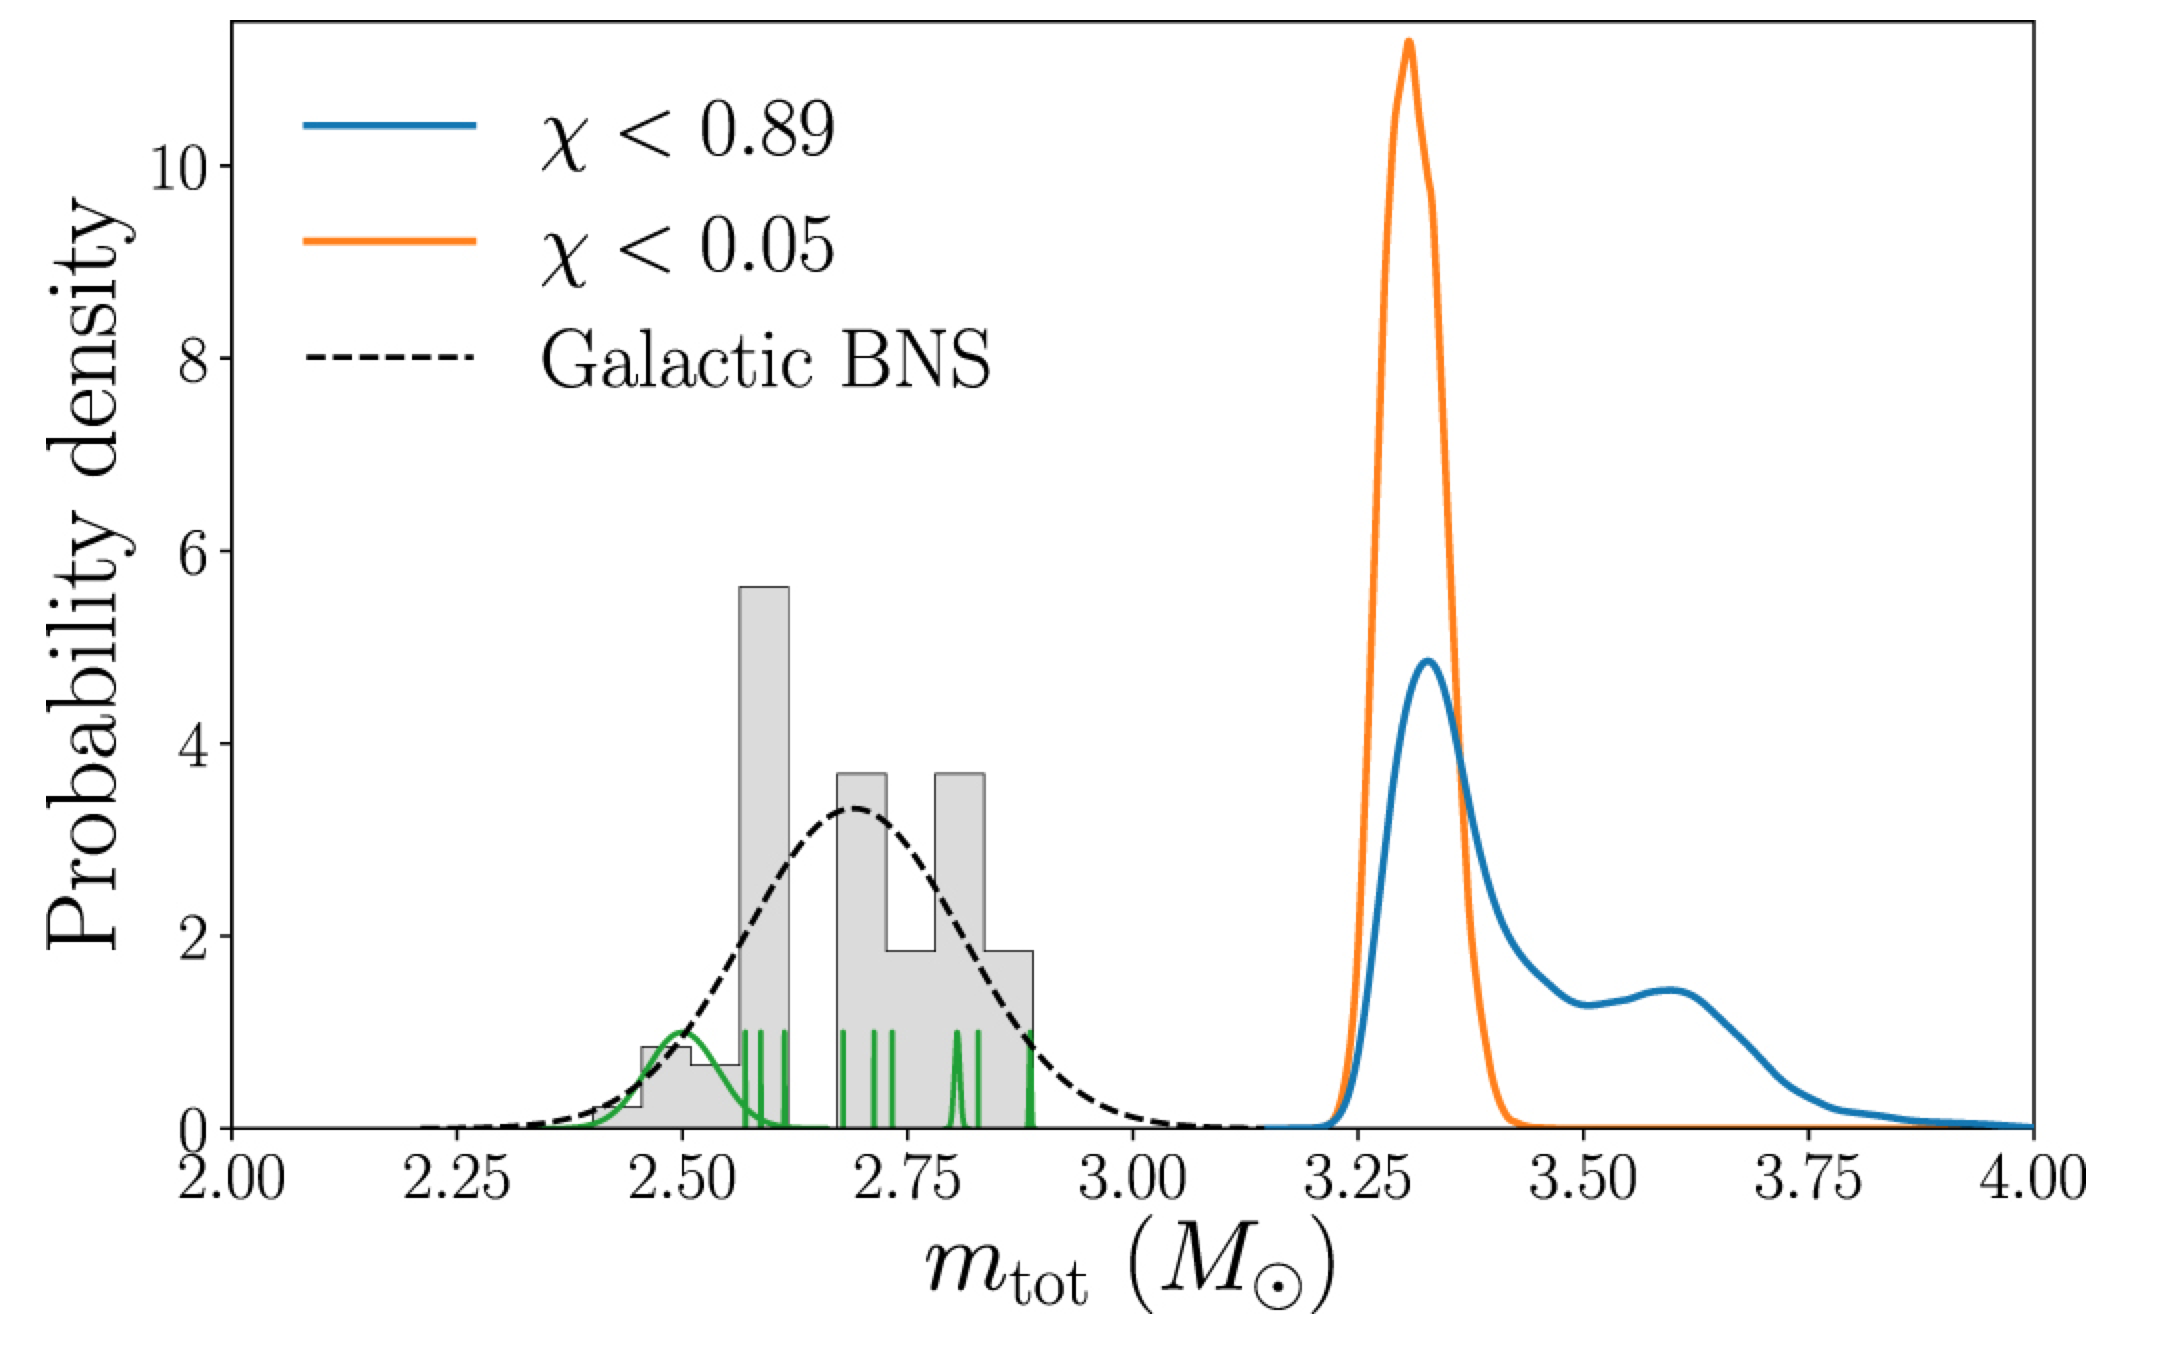
\includegraphics[scale=0.3]{secondbns}
          \centering
          \caption{Blue and orange curves are the total mass posteriors of GW190425 obtained by using different priors for the spins of the two NSs. In both cases, these distributions are dramatically different from the distribution of total masses of known galactic BNSs, reported with the grey histogram and fitted by the black dashed line. \cite{62}}
          \label{fig:secondbns}
        \end{figure}

	The unusual total mass of GW190425 may have implications for the origin of its source \cite{175}\fpg{Idem}.
	There are two ways in which we expect to form BNS. 
	Massive, fast-merging NS pairs could potentially result from 
	particularly low-metallicity stars evolving in close binary systems, undergoing a supernova explosion.
	If this is the case, GW190425 could be the representative of a population of BNSs never observed before, 
	because ultra-tight orbit NS systems with sub-hour periods are not detectable by current electromagnetic surveys.
	Another formation channel is the dynamical one: a third NS joins an already existing binary, 
	which could be a BNS or an NS with a main sequence star, kicking out the
	lower mass star and leaving behind a binary containing two NSs.

	The inferred NS spins are also consistent with the spins of the two fastest 
	spinning Galactic BNSs that are expected to merge within the lifetime of the Universe.

	In the BNS scenario, the detection of GW190425 provides an update 
	on the number of NS that collide in a volume of the universe every year, bringing this to $250$--$2810\,$Gpc$^{-3}\,$yr$^{-1}$ \cite{62}.

\subsection{GW190521: a 150-Solar-Mass Binary Black Hole Merger}
	The BBH that produced the GW event GW190521 was the most massive and energetic BH merger detected to date, 
	with masses of $85^{+21}_{-14}M_{\odot}$ and  $66^{+17}_{-18}M_{\odot}$.
	This event was detected with a three-detector network signal-to-noise ratio of 14.7, 
	and it is also the farthest source detected so far, with a luminosity distance of $5.3^{+2.4}_{-2.6}\,$Gpc,
	corresponding to an epoch when the universe was only about half its present age $z \sim 0.8$.

	The fact that the primary BH mass is $85 M_{\odot}$ is highly unusual, 
	since this is in conflict with current models of stellar evolution:
	based on the theoretical understanding of the internal workings of massive stars, 
	and how BHs form, we should expect to find BHs
	either with masses below $65M_\odot$ or higher than $120M_{\odot}$, but none in-between.
	The kinds of stars required to produce BHs in this gap would not follow the ``usual route,''
	going supernova, and thus would not end up forming BHs. 
	Rather, such stars would become unstable and get rid of a significant chunk of their mass. 
	Only then would they go supernova, but the result would be a BH of less than $65 M_\odot$.
	GW190521 suggests that either stars can form high mass black holes, 
	or that this is an example of ``hierarchical merger,'' 
	meaning the one or both BHs in the source were themselves the result of 
	a previous merger before they found each other and merged emitting GW190521.
	This multiple merger scenario requires that BHs form in special environments
        --- such as dense clusters of stars or the disks of active galactic nuclei --- 
	where there are enough other BHs nearby for multiple merger events to occur.

	A second groundbreaking discovery that came from this event 
	was the proof that intermediate-mass BHs do exist,
	since the mass of the BH remnant is $142^{+28}_{-16}M_\odot$, 
	falling right in the mass gap between stellar-mass and supermassive BH.

\subsection{GW190814: a Signal from an Unclear Source}
\label{subsec:GW190814}
	This was one of the must puzzling observations so far, as it is unclear
	whether its source was a BBH or an NSBH.
	This system shows the highest mass asymmetry observed to date:
	the primary component is a BH with mass $23.2^{+1.1}_{-1.0}M_\odot$, 
	while its companion has mass $2.59^{+0.08}_{-0.09}M_\odot$, right in the so called
	``lower mass gap.''  Therefore, it could either be the lightest BH
	observed so far, or the heaviest NS ever discovered in a binary.
        Notably this second mass is comparable to one of the remnant 
	produced by the merger of BNS source of GW170817.

	The lower mass gap originates from observations of X-ray binaries, 
	where there seems to be no BH below $\sim 5M_\odot$,
	a value also supported by theoretical predictions \cite{124}.
	The hypothesis that the unknown secondary object in GW190814 is indeed a BH, 
	requires an explanation for the lack of X-ray observation, 
	and for its production mechanism.
	On the other hand, another option is to assume that the NS mass upper limit is around $3M_\odot$.
	This, however, would be in tension with, among other things, the conclusion that 
        the maximum NS mass should be below $2.2$--$2.3M_\odot$, 
	a conclusion reached on the basis of the GW170817 observation \cite{122,123}.
	Therefore, the scenario in which the secondary object is a NS provides interesting new insights on the properties of NS matter, 
	as it requires a rather stiff equation of state with a maximum speed of sound $c_s \geq \sqrt{0.6}c$ \cite{121}.

	In principle, there are two possible ways of assessing whether or not a NS was present in the binary: 
	a measurement of the effects of the tidal distortion of the NS 
	in the GW signal, and/or the detection of an electromagnetic counterpart.
        Neither of these was successfully observed.
	Since tidal effects are suppressed by higher total masses 	
	and by unequal mass ratios, the measurement was inconclusive. 
	GW190814 was a three-detector detection, and the source localisation was tight ($18.5\,$deg$^2$.  
	However, it was located $\sim 240\,$Mpc away, that is,
	at six times the distance of GW170817.  
	This means that any light emitted would be about 36 times fainter in comparison to GW170817.
	Even if the event was a NSBH merger accompanied by an EM counterpart
	(see Sec.\,\ref{subsubsec:mrem_model} for the right conditions for this to happen), 
	the latter may have been too faint to be observed.

%----------------------------------------------------------------------------------------------------------------------------------------------------------------------------------------------------------
\chapter{Analyses of Data From the Third Observing Run}
\label{ch:datanalysis}
\fpg{Giri di correzione: 1.}%
\fpg{C'\`e ancora squilibrio in questa intro.  Ci devo lavorare.} %Posso rielaborarla, devo ridurre il prologo su NSBH? dire di più su data analysis?
        {\ttfamily PyGRB} is a GRB triggered CBC search
	which entails the coherent analysis of multiple detectors data as seen in Sec.\,\ref{subsec:coherent}. 
	It assesses whether a GW signal is present in the data, 
	given the time and sky position of an observed short GRB,
	by performing several signal-based veto cuts and data quality cuts.

	Not all compact binary mergers lead to the emission of an electromagnetic (EM) transient: 
	binary sources for which a multi-messenger emission is most probable are the ones that contain at least a NS.
	This is a minimum condition in order to have the presence of matter in the post-merger stage.
	However, a more stringent requirement is to demand
	the presence of matter resulting from the backwash of a BNS or an NSBH
	outside the remnant central BH.
	The evolution of this remnant matter can be responsible for the generation of several EM counterparts to GW events, and short GRBs in particular.
	Indeed, not all NSBH mergers are expected to emit electromagnetically and/or be viable short GRB progenitors (this is discussed further in Sec.\,\ref{sec:grbfollowup}).
	As a consequence, the parameter space which needs to be targetted by {\ttfamily PyGRB}
	is a subset of the CBC parameter space that excludes all systems that are \textit{EM-dim}:
	since short GRBs may be ignited when a sufficiently massive accretion disk forms around the remnant BH,
	the case of BBHs and of NSBH systems in which the NS plunges into the BHcan be excluded.
	This motivates the construction and use of 
	so called \textit{EM-bright} template banks for the matched filtering carried out by {\ttfamily PyGRB}.

	In order to build such template banks,
        it is of paramount importance to be able to estimate the amount of post-merger remnant matter as a useful indicator of 
	whether a coalescence is a potential GRB source.
	Several factors contribute to determining if and how much material is present after the merger, outside the BH,
        but an estimate is possible by exploiting fits to the results of
        numerical simulations of NSBH mergers.
	In the first part of this Chapter, we describe the implementation of a recent model \cite{54}, that accurately discriminates between parameter space 
	regions that enclose combinations of masses and spins that enable NSBH systems to be short GRB progenitor canidates.
        This implementation was used to generate the template bank adopted during the first part of the third LIGO-Virgo observing run (O3a) for {\ttfamily PyGRB} follow-ups of short GRB events.
	The resulting EM-bright template bank has been tested to assess its efficiency, as described in Sec.\,\ref{subsec:construction_and_validation}.
	We then present the results of the {\ttfamily PyGRB} analysis of three GRBs that occured during O3a, and 
	of the {\ttfamily PyCBC} of one chunk of data from the second part of the third observing run (O3b).

\section{Coherent Follow-Up of Short Gamma-Ray Bursts}
\label{sec:grbfollowup}
	The outstanding detection of GW170817 (Sec.\,\ref{subsec:GW170817}) 
        clearly demonstrated the vital importance of associating EM counterparts to GW triggers.
        Prior to this event, short GRBs had long been discussed as promising targets for GW astronomy,
        due to the probable compact binary nature of their progenitors \cite{154},
        a hypothesis which was confirmed by the joint detection of GW170817 and GRB 170817A.	

	Short GRBs and GWs 
	share the same catastrophic origin, 
	and are therefore tightly intertwined.
	Short GRBs represent an attractive target for GW follow-up searches. 
	The prior observation of a short GRB provides the time and sky position of a potential GW source. 
	The information about the short GRB observation, allows a targeted GW search for a compact binary signals to lower the detection threshold: thus,
        this kind of search has a higher sensitivity than
        and can uncover signals that are not accessible to
        a generic binary merger search, one that searches the whole sky at all times and for all compact binary mergers (including BBHs).
        Further, joint GW-GRB observations offer a unique means of probing the central engine of short GRBs.
        These are the scientific motivations for conducting GW follow-up searches of GRB events.

	Now that we have pinned down one class of short GRBs progenitors with GW170817, namely BNSs, 
	the next step is to observe the other likely short GRBs source: NSBH systems.
	Nevertheless, short GRB ignition is theoretically supported only by a fraction of NSBH mergers,
	specifically ones in which the BH tidally disrupts its companion, 
	and a sufficiently massive accretion disk forms around the remnant BH.

	From April 2019 to September 2019, the Advanced LIGO  and  Advanced  Virgo detectors undertook 
	the first part of the third observing run (O3a).
	{\rm PyGRB} was used to search for GWs associated with short and ambiguous duration GRBs detected by {\it Swift}/BAT or {\it Fermi}/GBM during O3a (see Introduction)\fpg{L\`i definisci short, ma non ambiguous.}.
	This required building and validating a template bank specifically designed for this task and then running the individual follow ups.  In the next Section I will describe the steps I carried out to deliver the bank and then I will report on the three GRB follow up analyses that I performed.

\subsection{The O3a Template Bank}
\label{subsec:o3aTemplateBank}
	As discussed in Sec.\,\ref{sec:template_banks}, running a modelled GW search 
	requires predetermining a set of waveform models, i.e., a template bank, in order to filter the data. 
	In opening Sec.\,\ref{sec:grbfollowup}, moreover, we linked BNS and NSBH systems to short GRBs as certain and potential progenitors, respectively.
	Additionally, studies have shown that a necessary and sufficient condition for an NSBH to emit an EM counterpart
	is to produce a sufficiently massive remnant accretion disk after the merger process \cite{176} \fpg{Undefined reference}.
	For these reasons, as of O1 included, {\ttfamily PyGRB} is run on detector data using a template bank
	that targets only BNSs and NSBH systems that produce a remnant accretion disk after merger \cite{55,136,161}, as suggested in \cite{162}.  This kind of template bank is often referred to as ``EM-bright bank,'' as it targets only potentially electromagnatically bright compact binary sources.

        Determining which NSBH systems may yield an accretion disk that surronds the remnant BH is possible via fits calibrated to numerical-relativity simulation results.  These fits take the NSBH binary physical parameters as input and return the mass of the accretion disk.
        The first fit of this kind was reported in \cite{50}.
	A more recent, remnant mass fitting formula was published in \cite{54}:
        part of this thesis was devoted to updating the code that generates EM-bright banks\footnote{\url{https://github.com/gwastro/pycbc/pull/3055}.}, producing the EM-bright bank for {\ttfamily PyGRB} follow ups of short GRB events that occured in O3a, and validating such template bank.
	The next sections describe these tasks step-by-step.

\subsubsection{Tidal Disruption of Neutron Star--Black Hole Binaries}
\label{subsubsec:mrem_model}
% 	The evolution of the BH singularity and the presence of matter combine
%         the difficulties of evolving both BBHs and BNS, and the system has its own specific challenges,
%         specifically the accretion of the NS matter onto the BH.
%         Such binaries are not only sources of GW radiation, but also potential sources of GRBs.
%         Since the first GW detection, the GW catalog has expanded collecting GW signals from BBH and BNS.
%         However, gravitational proof of the NSBH interaction is yet to be achieved:
%         this event would display a much richer phenomenology than BBH mergers,
%         even in the relatively simple case of both non-spinning objects.
%         From this last missing detection we are able to extract and learn about
%         the sources fundamental properties, such as the BH’s masses and spins
%         as well as the NS equation of state, because the orbital frequency at tidal disruption
%         depends strongly on the compactness of the NS, $C_{\rm NS}$ \cite{204};
%         from the electromagnetic radiation we can not only
%         pinpoint where the event happens but also withdraw informations about the events energetics as well as the environment.
%         Multi-messenger astronomy is like putting together the pieces of a cosmic puzzle
%         that allows us to understand CBC within the context of astrophysics cosmology and fundamental physics.
%         Detecting the GW signal associated to these systems is not only important for
%         GW astronomy but it is also an opportunity to observe a general relativistic system in the strong field regime,
%         in the presence of high-density nuclear matter, magnetic fields, shocks, and intense neutrino radiation.
%         This is the optimal scenario to validate whether NSBH binaries are suitable short GRBs progenitor canditate.

%\subsection{Tidal disruption model}
%\label{subsec:mrem}
        After the formation of an NSBH binary, the two companions go through a millions-of-years long inspiral phase,
        during which the binary separation gradually decreases and the orbit circularizes due to GW emission.
        As the BH and NS spiral in, the transition to a dynamically plunging orbit happens
        when the NS reaches either the innermost stable circular orbit, the radius of which we denote with $R_{\rm ISCO}$ of the BH, or the tidal disruption distance $d_{\rm tid}$,
        the distance at which the BH gravitational field is able to induce the tidal disruption of the star.
        Depending on the relative position of $R_{\rm ISCO}$ and the $d_{\rm tid}$ there are
        two\footnote{See, however, \cite{165} for a more detailed classification.} possible classes of events, as depicted in Fig.\,\ref{fig:nsbh}.
        If $d_{\rm tid} \lesssim R_{\rm ISCO}$, the NS plunges into the BH, no matter is left outside the remnant BH,
        and the chances of producing an EM counterpart are very low; in this case the GW signal is practically identical to the one emitted by a BBH system with the same component masses and spins \cite{163, 164, 165, 166, 167}.
        On the other hand, if $d_{\rm tid} \gtrsim R_{\rm ISCO}$, the NS will be disrupted by the BH tidal field, some debris may remain outside the BH after merger, and an accretion disk surrounding the remnant BH may form.
        When this matter is present outside the final BH, EM emission is expected to emerge from a variety of processes, e.g., \cite{169}.
        The mass of the remnant accretion disk, also depends upon the NS radius $R_{\rm NS}$, as suggested in \cite{168}.
        In this case the GW signal differs from the one of a BBH system with identical mass and spin parameters.
        \begin{figure}[!t]
          \label{nsbh}
          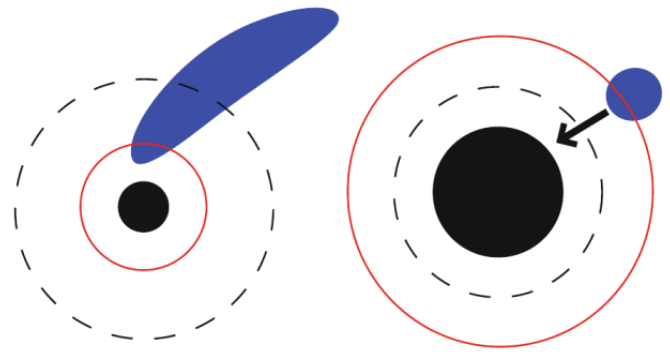
\includegraphics[scale=0.45]{nsbh}
          \centering
          \caption{{\bf The two main faiths of an NSBH binary.} Left: If the tidal disruption distance (dashed orbit) is larger than the radius of the innermost stable circular orbit (red, continuous orbit), the NS is disrupted and may form an accretion disk surrounding the remnant BH.  Right: Otherwise the merger ends with the plung of the NS onto its BH companion.}
          \label{fig:nsbh}
        \end{figure}

        All in all, the features of both the GW emission and its possible EM counterparts depend crucially on tidal disruption.
        This occurs when the tidal force of the BH at the surface of the NS exceeds 
        the NS self-gravity. Assuming Newtonian gravity, this condition is approximately given by
        \begin{equation}
          {{M_{\rm NS}} \over {R_{\rm NS}^2}} \sim {{3M_{\rm BH}} \over {d_{\rm tid}^3}}R_{\rm NS}\,,
        \end{equation}
        from simply $d_{\rm tid} \sim (M_{\rm BH}/M_{\rm NS})^{1/3}R_{\rm NS}$.
	Many factors influence the tidal disruption of the NS and hence the mass of the accretion disk that may form following it. 
	It is more likely that the NS will be swallowed directly by a more massive BH, 
	since it exerts weaker tidal forces at the ISCO;
	a highly  spinning BH has the effect of reducing the ISCO radius,
	possibly beyond the NS Roche limit.
	Furthermore, the NS equation of state has an impact:
	the softer the equation of state, the larger the NS radius, the higher the mass of the accretion disk,
	since the tidal force acting across the diameter of the star will be greater.

        A few tens of milliseconds after tidal disruption occurs the remnant consists of
        a remnant BH and tidal debris containing gravitationally bound and unbound matter.
        Some of the material gravitationally bound to the remnant BH swerves
        around it into an approximately axisymmetric disk, while some debris material,
        which is mostly neutron-rich, is dynamically ejected and spread outwards at mildly relativistic speeds.
	The accretion disk can spread to larger radii to conserve angular momentum in the rotational period $\sim 10\,$ms,
        rather than being confined within the circularizing radius, resulting in a gradual mass infall into the BH over longer timescales, $\sim 0.1-1\,$s.
        However, the mass accretion time scale is much longer than the rotational period, and hence, the disk remains quasi-stationary for $\gg 10\,$ms.
        With the intention of obtaining accurate predictions for identifying and characterising NSBH mergers
        a model for the remnant mass outside the BH is needed.

        Since NSBH systems cover a high-dimensional and largely unconstrained parameter space,
        understanding whether or not these events can result in short GRB emission requires to
        derive limits on the range of binary parameters leading to the disruption of an NS.
        Foucart (2012) \cite{50} proposed a model to calculate the amount of matter remaining
        outside the BH about $10\,$ms after an NSBH merger, $M_{\rm rem}$, based on a comparison
        between $d_{\rm tid}$, $R_{\rm ISCO}$, and $R_{\rm NS}$:
        \begin{equation}
          \label{eq:mrem}
          {{M_{\rm rem}^{\rm model}} \over {M^b_{\rm NS}}} = \alpha(3q)^{1/3}(1 - 2C_{\rm NS}) - \beta{{R_{\rm ISCO}} \over {R_{\rm NS}}}
        \end{equation}
        where $M^b_{\rm NS}$ is the baryon mass of the NS, $\alpha$ and $\beta$ are the free parameters of the model,
        $q=M_{\rm BH}/M_{\rm NS}$, which is equal to $\sim d_{\rm tid}$ in Newtonian gravity, and $C_{\rm NS} = M_{\rm NS}/R_{\rm NS}$ is the NS compactness. 
        This simple model applies to NSBH binaries with BH spins aligned with the orbital angular momentum and remnants below
        $\sim 25\%$ of the NS mass, leaving out parameter space regions which ath the time were unexplored by simulations, 
        namely high mass ratios, high BH spin magnitudes, and (moderately) spinning NSs.

        The model for $M_{\rm rem}$ was upgraded by Foucart and collaborators (2018) \cite{54}, who proposed:
        \begin{equation}
          \label{eq:mremup}
          {{M_{\rm rem}^{\rm model}} \over {M^b_{\rm NS}}} = \Bigg[ \max \Bigg( \alpha{{1 - 2C_{\rm NS}} \over {\eta^{1/3}}} - \beta {{R_{\rm ISCO}C_{\rm NS}} \over{\eta M_{\rm BH}}} + \gamma, 0 \Bigg)\Bigg]^{\delta}
        \end{equation}
        where $\alpha$, $\beta$, $\gamma$ and $\delta$ are the free parameter of the new model, and $\eta = q/(1+q)^2$ is the symmetric mass ratio of the binary.  The fitting parameters are found to be
	\begin{equation}
		\alpha=0.406, \hspace*{0.5cm}  \beta=0.139, \hspace*{0.5cm}  \gamma=0.255, \hspace*{0.5cm} \delta=1.761\,.
	\end{equation}

        Both models rely on considerations on tidal disruption dynamics and
        their free parameters were fitted to a set of numerical simulations.
        The first model in Eq.\,(\ref{eq:mrem}) was tested against 26 numerical simulations covering mass ratios
        in the range $q\in [3,7]$, $\chi_{\rm BH}\leq 0.9$, and $R_{\rm NS} \approx 11$-$16\,$km,
        while the more recent model in Eq.\,(\ref{eq:mremup}) was fitted to 75 simulations covering the range $q\in [1,7]$, $-0.5 \leq \chi_{\rm BH}\leq 0.97$,
        and $C_{\rm NS} = 0.13$-$0.182$.

\subsubsection{Construction and Validation}
\label{subsec:construction_and_validation}
	In light of the discussion so far, an EM-bright bank cover the portion of compact binary parameter space that
        corresponds mass and spin combinations, such that one is in presence either of a BNS or of an NSBH that will yield an accretion disk after the merger.
        \begin{itemize}
        \item While most NS observed in BNS systems have masses in the $[1.2, 1.6]M_{\odot}$ range \cite{87},
          more massive NSs exist and have been found either in isoltation with radio obsservations ($\sim 2\,M_{\odot}$ \cite{87}) or in binaries with GW observations (see, e.g., Sec\,\ref{subsec:GW190425}).  Above $3.2\,M_\odot$ non-rotating, isotropic NSs imply a violation of causality and cannot exist, according to our present understanding of these objects.
          The maximum mass depends on the equation of state chosen for the NS interior.  We pick the 2H piecewise polytropic equation of state \cite{170} that yields a maximum viable NS mass of $\sim 2.8M_\odot$ and high NS compactnesses (radii of about 15 to 16\,km), which favours NS tidal disruption [see Eq.\,(\ref{eq:mremup})]: both implications of this equation of state are inclusive in terms of parameter space we need to cover with an EM-bright bank.
          In summary, we target the NS mass interval $1M_\odot$-$2.8\,M_\odot$.
        \item Galactic BHs have masses that fall in the interval $[5,-15]M_{\odot}$ \cite{124},
          but GW observations have involved BHs with higher masses \cite{49}.
          Further, in Sec.\,\ref{subsec:GW190814} we mentioned the ``lower mass'' gap $3$-$5M_\odot$ that may separate NSs from BHs, so there is some freedom in setting both the lower and upper limit of the BH masses we decide to target.
          We chose to cover BH masses in the range $[2.8,25]M_\odot$.
          This provides continuity with the NS mass values on the lower end, while on the higher end the choice is motivated by the fact that forming accretion disks according to Eq.\,(\ref{eq:mremup}) becomes very difficult, as it requires very high BH spins or even unphysical spin values (depending on the NS equation of state that one chooses).  Further at the high-end of this mass interval, one has NSBH systems with mass ratios between $9$ and $25$, and the highest BBH mass ratio recorded so far is $\sim 10$ (Sec.\,\ref{subsec:GW190814}).  In light of these considerations and of the fact the uncertainty on gravitational-waveform models increases with the mass ratio, $25M_\odot$ is physically a more than reasonable upper limit for the BH mass.
        \item The maximum dimensionless spin magnitude for BHs is set to 0.998 (just below the Kerr limit), while for NSs it is set to 0.05, as dictated by known galactic BNS systems \cite{97}.  The spins in the templates are taken to be aligned with the orbital angular momentum as a coherent search that includes precession has not been implemented yet.
        \item Most BNS and NSBH binaries
        are expected to have negligible eccentricities once they enter the band of terrestrial IFOs \cite{86}.
        While eccentric NSBH binaries cannot entirely be ruled out
        and have evolutions that are distinct from circular ones \cite{71},
        the template bank is designed assuming zero eccentricity.
      \end{itemize}

      Two other parameters must be specified in order to generate the bank.  
	1) The design value for the minimum match \fpg{Se prima dicevamo overlap, qui dobbiamo dire overlap. Controllare.} of the bank with any point in its target paremeter space, which is set to $0.97$, allowing for at most 10\% signal losses.\footnote{The detection rate is proportional to the cube of the SNR, and the SNR is proportional to the match, which is 0.97 in the worst case scenario.}  Matches are calculated over the frequency interval $[27, 1000]\,$Hz. 2) The threshold value for the accretion disk mass of NSBH binaries that flags them as potential short GRB progenitors: any NSBH with $M_{\rm rem}>0$ is considered as a viable short GRB progenitor, in order to err on the side of caution thus including more NSBH binaries than necessary, rather than risk omotting them.
      Finally, we must specify the model to generate gravitational waveforms and compare them.  We used the phenomenological model for spinning, non-precessing binaries {\ttfamily IMRPhenomD} \cite{106}.  This mdoel does not account for NS-specific contributions to the waveform: the presence of NSs therefore enters our bank only via the fitting formula used to calculate $M_{\rm rem}$ and downselect NSBH binaries that are viable short GRB progentors.

      The EM-bright bank is generated with a hybrid placement code (see Sec.\,\ref{subsubsec:HybridBank}).  At every proposal of a new point in the parameter space, the bank generation algorithm must determine whether to add or not that proal to the set of tempalate points.  Based on the two masses of the proposed new bank element, three things may happen. 
      \begin{enumerate}
        \item If both masses are at most $2.8M_\odot$, then the point is treated as a BNS representative, which is automatically a potential short GRB progenitor and it therefore added to the bank if the match of its corresponding GW with all other GWs already in the bank is lower than the $0.97$ design threshold.
        \item If both masses are larger than $2.8M_\odot$, the point is treated as a BBH representative, which is automatically discareded as it may not power a short GRB.
        \item If only one of the two masses is below $2.8M_\odot$, then the point is taken to represent an NSBH binary. In this case Eq.\,(\ref{eq:mremup}) is run on the physical parameters of the system.  If $M_{\rm rem}^{\rm model}=0$, the point is discarded, as the binary merger cannot lead to a short GRB.  Otherwise, namely if $M_{\rm rem}^{\rm model}>0$, the GW for that point is generated and its minimum match against all other waveforms in the bank is determined.  If this does not exceed the 0.97 threshold value, the point is added to the bank, otherwise it is not.
        \end{enumerate}
% 	\item The new template bank generates a large set of point within the mass and spin parameter space,
%         with the desired minimum $M_{\rm rem}$, then it checks if the systems produce an EM counterpart.
%         This means they are required to produce a remnant mass disk:
%         if they do equation of state data are loaded and the minimum $\eta$ needed to generate a given $M_{\rm rem}$,
%         as a function of $M_{\rm NS}$ and $\chi_{\rm BH}$,  is computed;
%         if this is not the case the binary is treated as point particle binaries.
%         All system that produce the given $M_{\rm rem}$ make the cut and are stored:
%         as the EM cut can remove several randomly generated binaries,
%         the numbers of accepted points needs to be tracked and stopped when they are enough.
%         \item First all EM dark systems needs to be identified using the logical mask ‘\textbf{{\color{red}mask\_not\_bbh}},
%         which track points that are not BBH: a point is kept if the secondary object is not a BH,
%         then its masses and spins are stored.
%         After this first cut only BNS and NSBH systems are left.
%         \item To discriminate between these two classes, another requirement is that the secondary mass is a NS,
%         so that ‘\textbf{{\color{green}mask\_bns}}’ identifies only BNS, while the systems that do not satisfy this conditions
%         are identified by ‘\textbf{{\color{black}masknsbh}}’.
%         All these point’s masses and spin are stored.
%         \item As previously showed in Sec.\,\ref{subsubsec:mrem_model}, not all NSBH coalescence produce an EM counterpart,
%         so the next step is to keep only those systems whose $M_{\rm rem}$ is greater than the threshold mass to have a counterpart,
%         identify these points with ‘\textbf{{\color{blue}mask\_nsbh\_bright}}’ and store their masses and spins.
% 	\end{itemize}
%\begin{table}[H]
%\noindent
%\begin{tabular}{|l|l|l|l|l|} \hline
%\textbf{BNS}  & \textbf{NSBH}       & \textbf{NSBH}    & \textbf{BBH}     \\
%EM-bright     & EM-bright  & EM-dim  & EM-dim  \\\hline
%{\color{red}1}0{\color{green}1}  & {\color{red}1}1{\color{green}0}{\color{blue}1}  & {\color{red}1}1{\color{green}0}{\color{blue}0}  & {\color{red}0}  \\ \hline
%\end{tabular}
%\end{table}

	The O3a EM-bright template bank produced once the code was able to hande Eq.\,(\ref{eq:mremup}) contained 288,177 templates and is shown in Fig.\,\ref{fig:banktest}.  The two axes represent the mass of the BH and the magnitude of its spin, while the color code is the NS mass.  The only information lost in this plot is the NS spin magnitude, but this is taken to be 0.05 at most, so this direction in parameter space is not very rich.
        A significant portion of the parameter space is empty of any templates  (lower-right),
        as it either contains BBH systems or NSBH systems that cannot produce an accretion disk around the BH remnant.
        Another advantage emerges at this point, as this is the portion of parameter space where waveforms mostly latch onto detector noise transients.  The absence of template points here translates into an increase in sensitivity for the {\rm PyGRB} search.

        \begin{figure}[t]
          \noindent
          \label{banktest}
          \makebox[\textwidth]{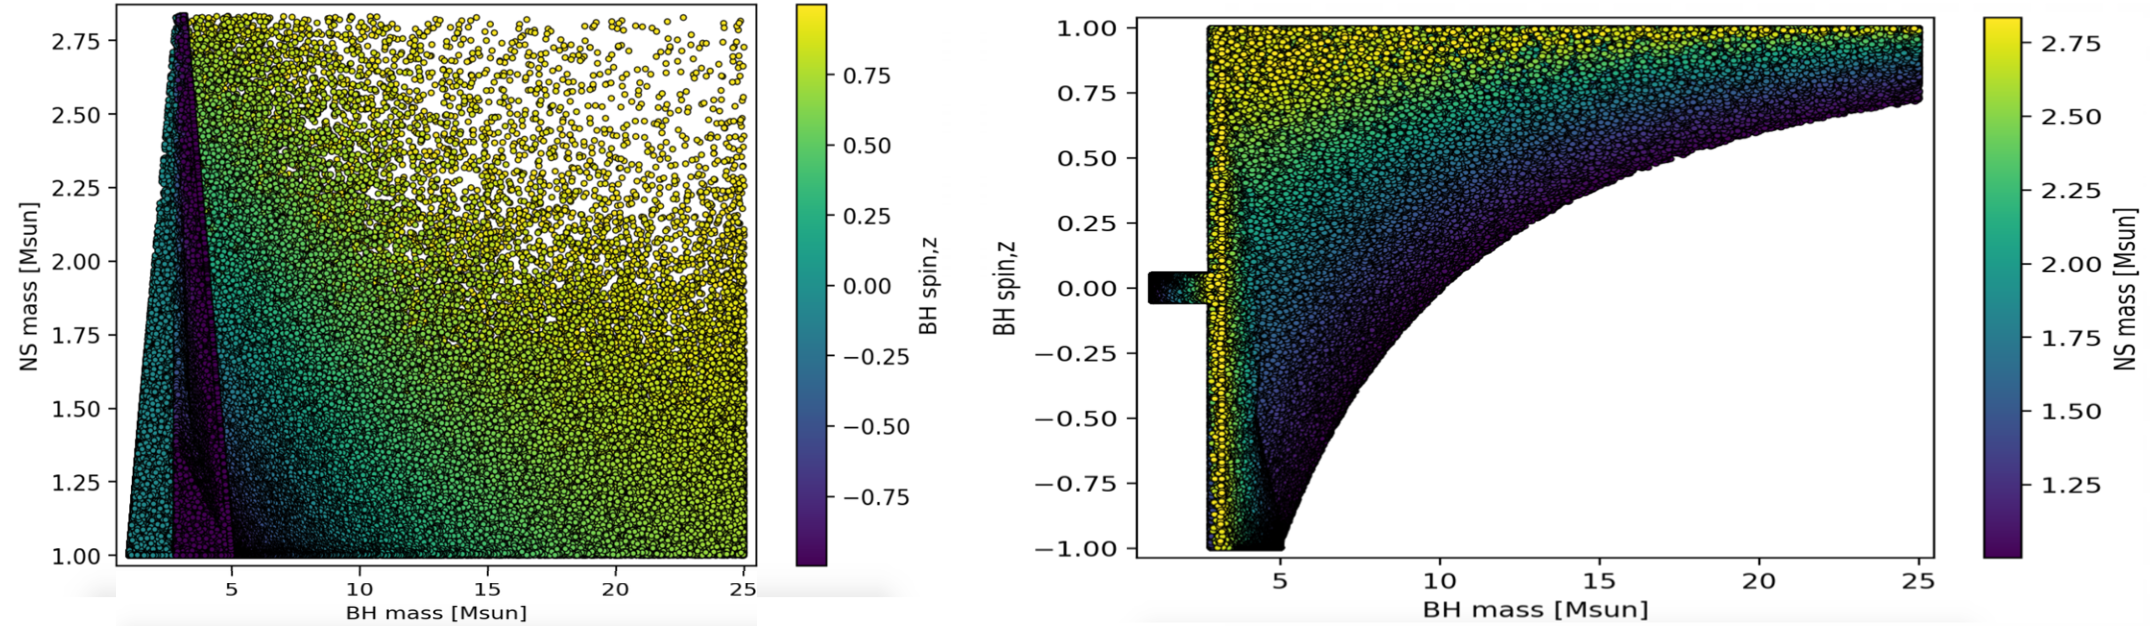
\includegraphics[scale=0.45]{banktest}}%
          \centering
          \caption{{\bf The O3a template bank for the GW follow up of short GRBs.} The horizantal and vertical axis are the BH mass and dimensionless spin magnitude, respectively.  The colorcode is based on the NS mass.}
          \label{fig:banktest}
        \end{figure}

        \begin{figure}[!t]
          \noindent
          \makebox[\textwidth]{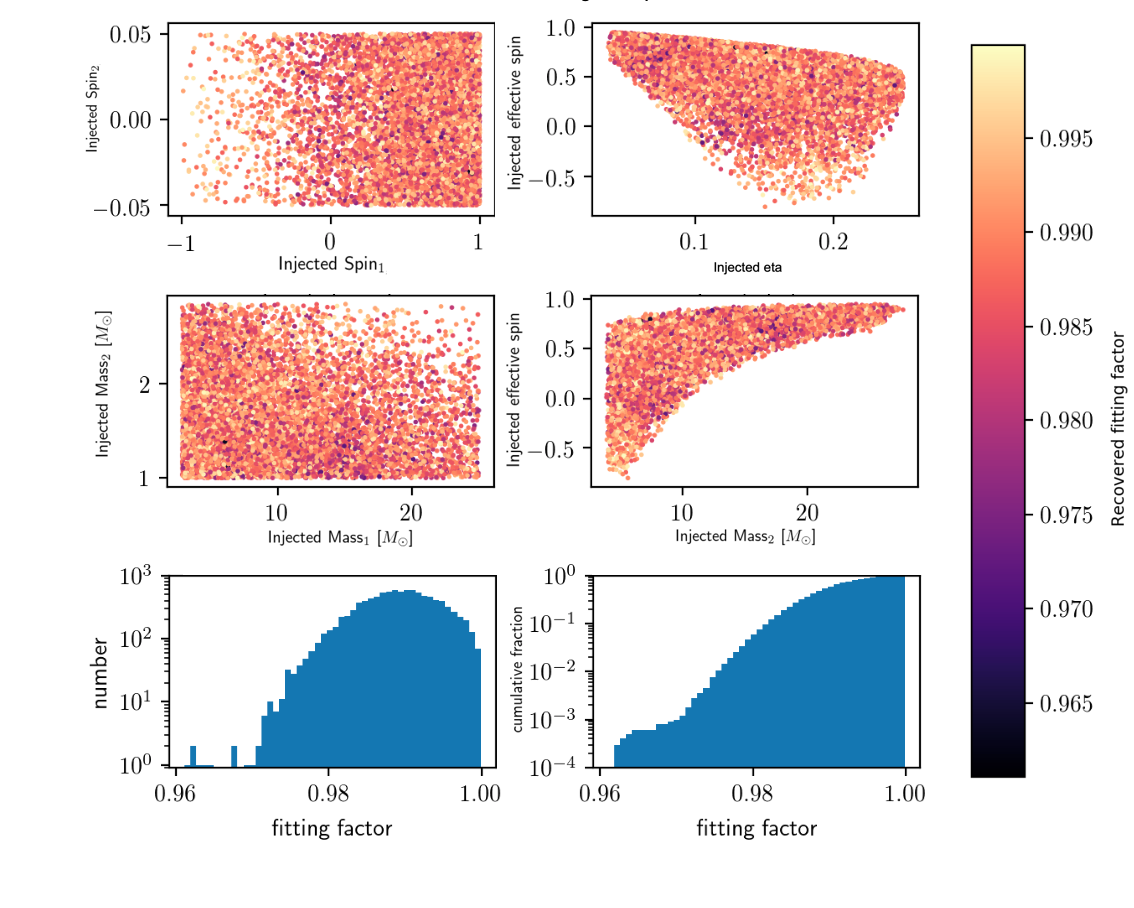
\includegraphics[scale=0.7]{fittingfactor}}%
          \centering
          \caption{{\bf Recovery of NSBH injections with the O3a {\ttfamily PyGRB}-dedicated template bank.}  In the scatter plots, from left to right and top to bottom, the fitting factors are reported as a function of: the BH and NS dimensionless spin magnitudes; the symmetric mass ratio and the effective dimensionless spin (a mass-weighted combination of the two dimensionless spin components); the BH and the NS masses; the NS mass and the effective dimensionless spin.  The bottom histograms show the distribution and cumulative distribution of the fitting factor values.  Roughly 0.001 of the injections are recovered with match smaller than 0.97.}
          \label{fig:fittingfactor}
        \end{figure}

	Once a bank is built, it is important to check that it actually covers appropriately the region of interest in parameter space, with the required minimum match tollerance of 0.97.
        This is known as testing the \emph{effectiveness} of the bank,
        which is done by calculating the fitting factor introduced in Sec.\,\ref{subsec:fittingfactor} for several simulated GW signals drawn within the target parameter space.
        Our first set of injected GW signals covered the target NSBH parameter space with 10,000 simulated waveforms.
        This set is subject to the same EM-bright condition used to build the template bank, namely, all injections are require to have $M_{\rm rem}^{\rm model}>0$ according to Eq.\,(\ref{eq:mremup}).
        A second set, also of 10,000 injections, covered the target BNS parameter space.
        All injected waveforms are generated using the effective-one-body waveform model {\ttfamily SEOBNRv4\_ROM} \cite{172}, which differs from the one used to construct the bank ({\ttfamily IMRPhenomD}).  The rationale is to factor in our uncertainty about the waveform by switching to a different model from templates to injections.

        Results for the recovery of the two injection sets just described are reported in Figs.\,\ref{fig:fittingfactor} and \ref{fig:fittingfactorBNS}.  In both cases, only about a thousandth of the injections are recovered with match smaller than 0.97.  The small tail in the fitting factor distribution for the NSBH injection sets is due to differences between the waveform models {\ttfamily SEOBNRv4\_ROM} (for the injections) and {\ttfamily IMRPhenomD} (for the templates), which emerge for high spins and mass ratios.  Importantly, none of the scatter plots presents areas in which points with lower fitting factors tend to cluster:
        this means that there are no ``holes'' in the banks, or systematics in the placement of templates by the algorithm.
	The average fitting factor for the entire bank is $\sim0.98$, meaning a $\sim 6\%$ loss of detections: this is smaller than the 10\% goal we had set, so the bank passes the validation, or effectiveness, test.  \fpg{Lo 0.98 come lo hai ricavato? A quale set si riferisce? BNS o NSBH?  E qual \`e il valore per l'altro set?}

        \begin{figure}[!t]
          \noindent
          \makebox[\textwidth]{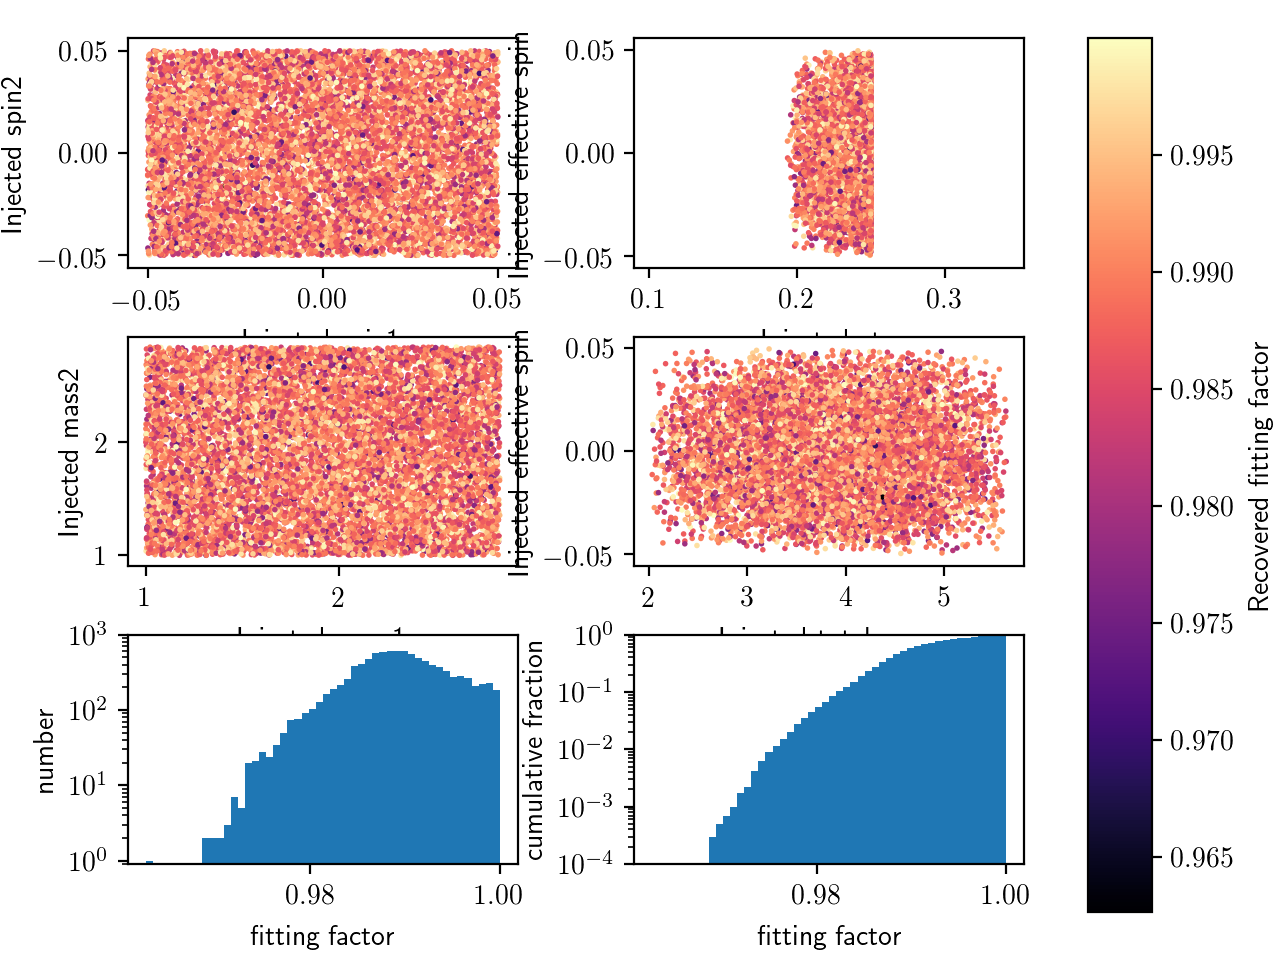
\includegraphics[scale=0.45]{HL-BANKSIM_PLOT_FITTING_FACTORS_BROADINJBNS1_MAIN-2620801-1163865616}}%
          \centering
          \caption{{\bf Recovery of BNS injections with the O3a {\ttfamily PyGRB}-dedicated template bank.}  This plot is similar to Fig.\,\ref{fig:fittingfactor}, but the physical parameters of the more massive object are drawn from NS, rather than BH, distributions.}
          \label{fig:fittingfactorBNS}
        \end{figure}

% 	In Fig.\,\ref{fig:pointinj}, results from an additional check for the bank validity are shown: 
% 	this is done by using point injections, wherein 10,000 signals are injected at single points in the mass parameter space while varying the spins. 
% 	For this set, 43 points in the mass parameter space were chosen randomly. 
% 	It confirms that the bank works well, as the lowest fitting factor of these points is 0.9870, 
% 	which is consistent with the bank average from the broad injection set. 
%                 \begin{figure}[!t]
%                         \noindent
%                         \label{pointinj}
%                         \makebox[\textwidth]{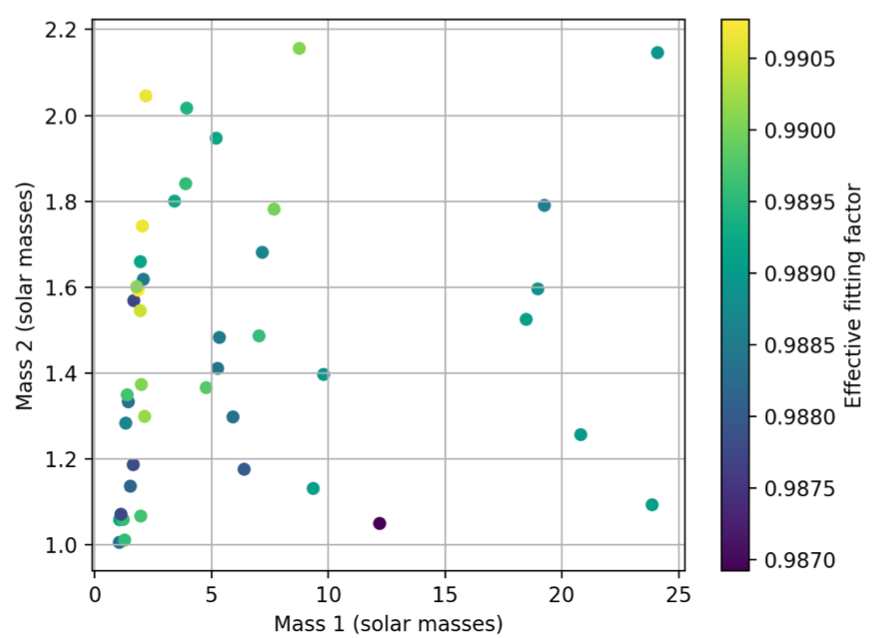
\includegraphics[scale=0.55]{pointinj}}%
%                         \centg
%                         \caption{The effective fitting factor is the signal-strength weighted average fitting factor. This is shown, as a function of masses, for the input injection sets. Injections are filtered so that only those passing the filter function used when creating the input files are considered. Usually this is used to restrict to only signals that are the parameter space used to create the template bank. Any point marked with a black cross contain no injections that pass the filter function.}
%                         \label{fig:pointinj}
%                 \end{figure}

\subsection{Setup of the Offline Analysis}
\label{subsec:pygrb}
	The {\ttfamily PyGRB} pipeline performs a targeted search for CBC GW signals in LIGO and Virgo data associated with short GRBs seen by {\it Swift}/BAT and {\it Fermi}/GBM,
        using the known sky location of the short GRB and the relative GW detector sensitivities to analyses the data coherently, as described in Sec.\,\ref{subsec:coherent}.
        Even though this approach is more computationally expensive than a coincident search, described in Sec.\,\ref{subsec:coincident},
        it is more sensitive.
	The analysis is performed if the GW data cover a period of time on either side of the short GRB that is long enough to build the background of the search.  The typical requirement is half an hour of data.
	The pipeline looks for a GW signal in a time window, ``on-source,'' that runs from 5\,s before to 1\,s 
	after the Earth crossing time of the short GRB \cite{92, 136}.
	However,
        the additional data surrounding the on-source time and required to characterize the detector sensitivity at the time of the GRB event
	is referred to as the ``off-source window.''

	The first part of the analysis consists in matched-filtering the individual detector data.%;
%	knowing the GRB sky location and the fact that GWs travel at the speed of light,
%	data from each detector is time-shifted so that there is a temporal coincidence between the GW and the GRB in each IFO \cite{92}.
	A list of GW triggers is assembled by keeping only times when the individual detector $\rho > 4$.
	Further trigger selection is accomplished by rejecting any trigger with $\rho_{\rm coinc}<6$ [see Eq.\,(\ref{eq:rhocoinc})].
        The coherent SNR is also calculated and triggers are downselected by requiring $\rho_{\rm coh}>0$ [see Eq.\,(\ref{eq:rhocoh})].
	The final SNR cut is performed by computing $\rho_{\rm null}$ [see Eq.\,(\ref{eq:rhonull})] and keeping only the triggers that satisfy the following conditions \cite{46}:
        \begin{equation}
          \begin{cases}
            \rho_{\rm null} \leq 5.25 & \wedge ~~~ \rho_{\rm coh} \leq 20\\
            \rho_{\rm null} \leq {{\rho_{\rm coh}-20}\over {5}} & \wedge ~~~ \rho_{\rm coh} > 20
          \end{cases}\,.
        \end{equation}
	This prevents us from losing possibile loud GW events with high $\rho_{\rm null}$.
	The high null SNR in this case may stem from differences between the actual gravitational waveform and the waveform model of the template used for the matched filter, 
	as well as from inaccuracies in the timing and/or sky position, which can lead to some fraction of the energy of a GW contributing to the null SNR. 	

	In order to remove glitches --- which may also have high SNR values --- the remaining triggers go through the $\chi^2$-test described in Sec.\,\ref{subsubsec:multidec_chi_test}.
	Once the final list of triggers is ready, they need to be ranked in order of likelihood of being a real GW event:
	the SNR of the surviving triggers are thus re-weighted based on the values of their $\chi^2$-tests and null SNR.
	This allows us to downweight glitches that still pass the previous cuts.
	The re-weighting is carried out in two steps: first according to the $\chi^2$ value,
        \begin{equation}
          \begin{cases}
            \rho_{\chi^2} =  \rho_{\rm coh} & \text{if}~~ \chi^2 \leq n_{\rm dof} \\
            \rho_{\chi^2} =  {{\rho_{\rm coh}}  \over {\{[1+ \big( {{\chi^2} \over {n_{\rm dof}}} \big)^3 ]/2\}^{1/6}}} & \text{if}~~ \chi^2 > n_{\rm dof}
          \end{cases}\,,
        \end{equation}
	and then according to the null SNR value:
        \begin{equation}
          \begin{cases}
            \rho_{\rm rw} = \rho_{\chi^2} & \text{if}~~ \rho_{\rm null} \leq 4.25\\
            \rho_{\rm rw} = {{ \rho_{\chi^2}}  \over {\rho_{\rm null} - 3.25}} & \text{if}~~ \rho_{\rm null} > 4.25
          \end{cases}\,.
        \end{equation}
	In order to remove non-Gaussian noise transients left in trigger list, 
	any trigger with $\rho_{\rm rw}<6$ is discarded.
	The template yielding the largest $\rho_{\rm rw}$ 
	in the on-source window is retained \cite{46}. 
	For the {\ttfamily PyGRB} analysis, the threshold that must be exceeded in order for this loudest trigger to be promoted to candidate event is $\rho_{\rm rw} = 8$.

	The last step is to determine the significance of the loudest trigger trigger,
	namely how often random noise in the detector data can generate a trigger with $\rho_{\rm rw}$ equal to or higher than the loudest trigger surviving in the on-source.
	This is done by calculating the false alarm probability (FAP) around the time of the GRB, as discussed in Sec\,\ref{subsec:coherent}. \fpg{il discorso della coherent FAP va messo in 2.4.2 per simmetria con 2.4.1.  Qui rimarr\`a ``as discussed in Sec\,\ref{subsec:coherent}.''}

        The efficiency of the analysis is assessed by injecting simulated signals to the data stream and reperforming the search.
 	This also allows to place a lower bound on the distance to the short in the absence of a GW in the on-source window. 
        The simulated signals are drawn randomly from astrophysically motivated distributions of the CBC source parameters (masses, spins, and extrinsic parameters).
	Three sets of injections were performed in O3a.  A set of BNS signals and two sets of an NSBH signals, one with both spins aligned to the orbital angulare momentum (no precession) and one with generic spin orientations (with precession).  Since NS spin magnitudes are taken to be 0.4, at most, precession in the case of BNS systems is generally not too significant and therefore a single, precessing set is taken for BNSs, unlike NSBHs, for which the BH spin magnitude may reach up to 0.98.
	All simulated signals are modelled using the {\ttfamily SEOBNRv3} waveform approximant \cite{103,173,174}, which differs from the {\ttfamily IMRPhenomD} waveform model used to generate the templates: this is intentional and factors in our incomplete knowledge about waveforms.
	The injection parameters are chosen as follows \cite{43}.
        \begin{itemize}
        \item $M_{\rm BH}$ is drawn from a Gaussian distribution with mean $10M_\odot$ and width $6M_\odot$.
        \item $\chi_{\rm BH}$ is drawn uniformly in the interval $[0.00, 0.98]$.
        \item $M_{\rm NS}$ is drawn from a Gaussian distribution with mean $1.4M_\odot$, and width of $0.2M_\odot$ for BNS systems and $0.4M_\odot$ for NSBH systems.
          The larger width for NSBH binaries is chosen in order to reflect the greater uncertainty arising from a lack of observed NSBH systems. 
        \item For the two injection sets with generic spin orientations, both spin orientations are drawn uniformly on the solid angle. 
        \item Short GRB are considered to be emitted in the direction of the binary total angular momentum.
          Relativistic beaming and collimation due to the ambient medium confines the GRB jet to a half-opening angle. 
          The observation of prompt gamma-ray emission is, therefore, indicative that the inclination of the total angular momentum 
          with respect to the line of sight to the detectors lies within the jet cone.
          Therefore, for all three populations of injected signals,
          the inclination with respect to the line of sight is drawn from a uniform distribution in $[\ang{0}, \ang{30}] \cup [\ang{150}, \ang{180}]$.
        \item Finally, only injections corresponding to NSBH systems with $M_{\rm rem}^{\rm model}>0$ are considered.
        \end{itemize}
        The fraction of recovered simulated signals as a function of (simulated) source distance is recorded as a means of providing a measure of the pipeline performance 
	and of the lower limit to the source distance, i.e., an \emph{exclusion distance}.

\subsection{GRB 190627A}
	GRB 190627A was detected by the BAT onboard the {\it Swift} satellite on June 27, 2019, at 11:18:31 UTC.
	Its location was determined to be $RA=\ang{244.83}$, $Dec = \ang{-5.3}$, with 3 arcmin uncertainty.	
	The duration it had in the 15--350\,keV band was $T_{90} = 1.60 \pm 0.28$s, 
	which places it at the longer end of the short GRB distribution. 
	Follow-up electromagnetic observations of GRB 190627A detected its optical counterpart, 
	and by analysing the spectrum it was inferred that $z = 1.942$ is the likely redshift of this specific GRB.
	However, this falls beyond the detection range of the interferometers,  therefore no associated GW detection is  expected.

	At the time of GRB 190627A, two GW detectors, H1 and L1, 
	were operating and their responses in the direction of the GRB were 0.316 and 0.452, respectively.
	The panels in Fig.\,\ref{fig:signalconsistencyplots1} show the results 
	of the $\chi^2$-tests applied to the offsource background data (blue crosses), and to the injections (red crosses),
	the parameters of which are listed in Sec.\,\ref{subsec:pygrb}, that serve as a simulated foreground. 
	From top to bottom, the panels report the template bank veto test, 
	the autocorrelation veto test, and the standard $\chi^2$-test, 
	discussed in Sec.\,\ref{subsubsec:multidec_chi_test}, as a function of coherent SNR. 
	The contour lines correspond to values of constant re-weighted SNR.  
	The black line, in particular, has a value of 6, 
	which is the threshold value discussed in Sec.\,\ref{subsec:pygrb}.
	The shaded region is therefore vetoed: any triggers that fall within it 
	will fail that specific $\chi^2$-test and be discarded.
	The effect of non-stationarities in the data is evident in the first two plots, 
	that clearly show several background triggers with high coherent SNR \emph{and} high $\chi^2$ values.  
	When an injection overlaps with a glitch in the background, 
	it may be dragged in the veto area and therefore be missed, as seen from the plots, 	
	particularly for a single missed injection with coherent SNR $\sim 12$.  
	This behaviour is not surprising and corresponds to situations in which a physical GW signal 
	can overlap with a noise transient and thus not be confidently detected.
        \begin{figure}[!t]
          \noindent
          \label{signalconsistencyplots1}
          \makebox[\textwidth]{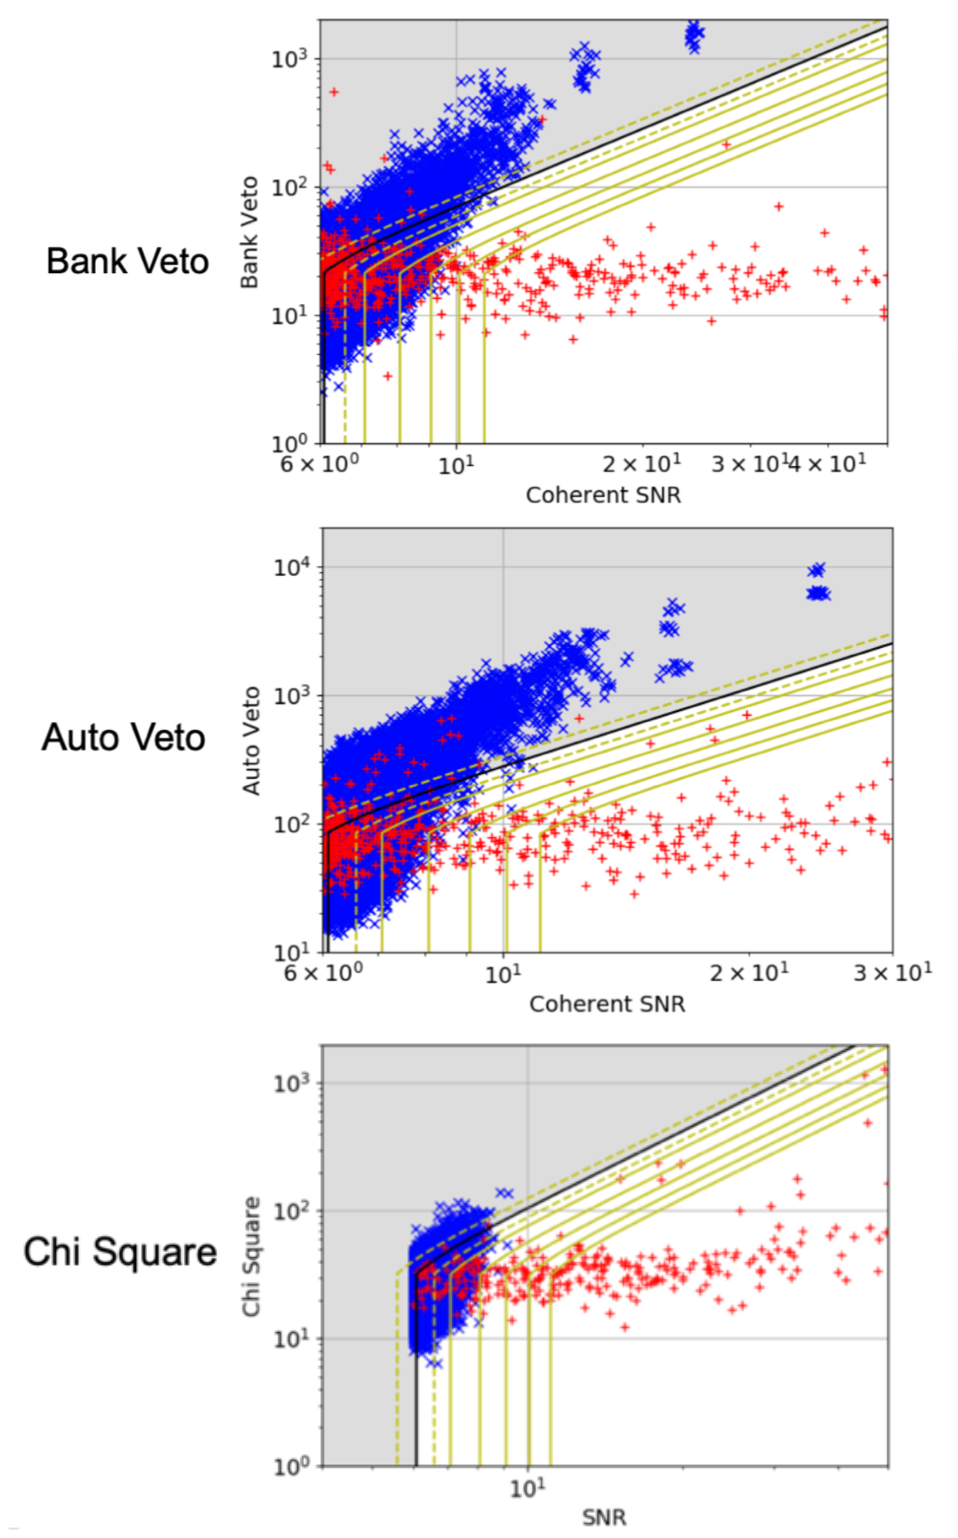
\includegraphics[scale=0.68]{signalconsistencyplots1}}%
          \centering
          \caption{\textbf{$\chi^2$ signal consistency plots.} The panels show the $\chi^2$-test results for background data (blue crosses) and injected signals (red crosses) as a function of coherent SNR.   From top to bottom, the test reported are: the template bank test (``Bank Veto''), the autocorrelation test (``Auto Veto''), and the standard, frequency bin $\chi^2$-test (``Chi Square'').   The yellow lines mark contours of constant re-weighted SNR. See Sec.\,\ref{subsubsec:multidec_chi_test} for details on the three $\chi^2$-tests.}
          \label{fig:signalconsistencyplots1}
       	\end{figure}
	Additional signal consistency tests are reported in Fig.\,\ref{fig:detector1}. 
	Here, the single detector SNR is shown as a function of the coherent SNR, 
	for the background data and injected signals (blue and red crosses, respectively).
	The expected trend for astrophysical signals is given by the middle, green line, 
	whereas the other two green lines, the magenta lines, and the cyan lines represent $1\sigma$, $2\sigma$, 
	and $3\sigma$ deviations, respectively.
	The behaviour of H1, which in this case is less sensitive than L1, 
	is qualitatively worse but still acceptable.  
	The background data clearly depart from the expected behaviour of astrophysical signals.
        
	Finally, the black horizontal line and the shaded area beneath it mark a search threshold 
	that is no logner used, so we will not discuss it.
        \begin{figure}[!t]
          \noindent
          \label{detector1}
          \makebox[\textwidth]{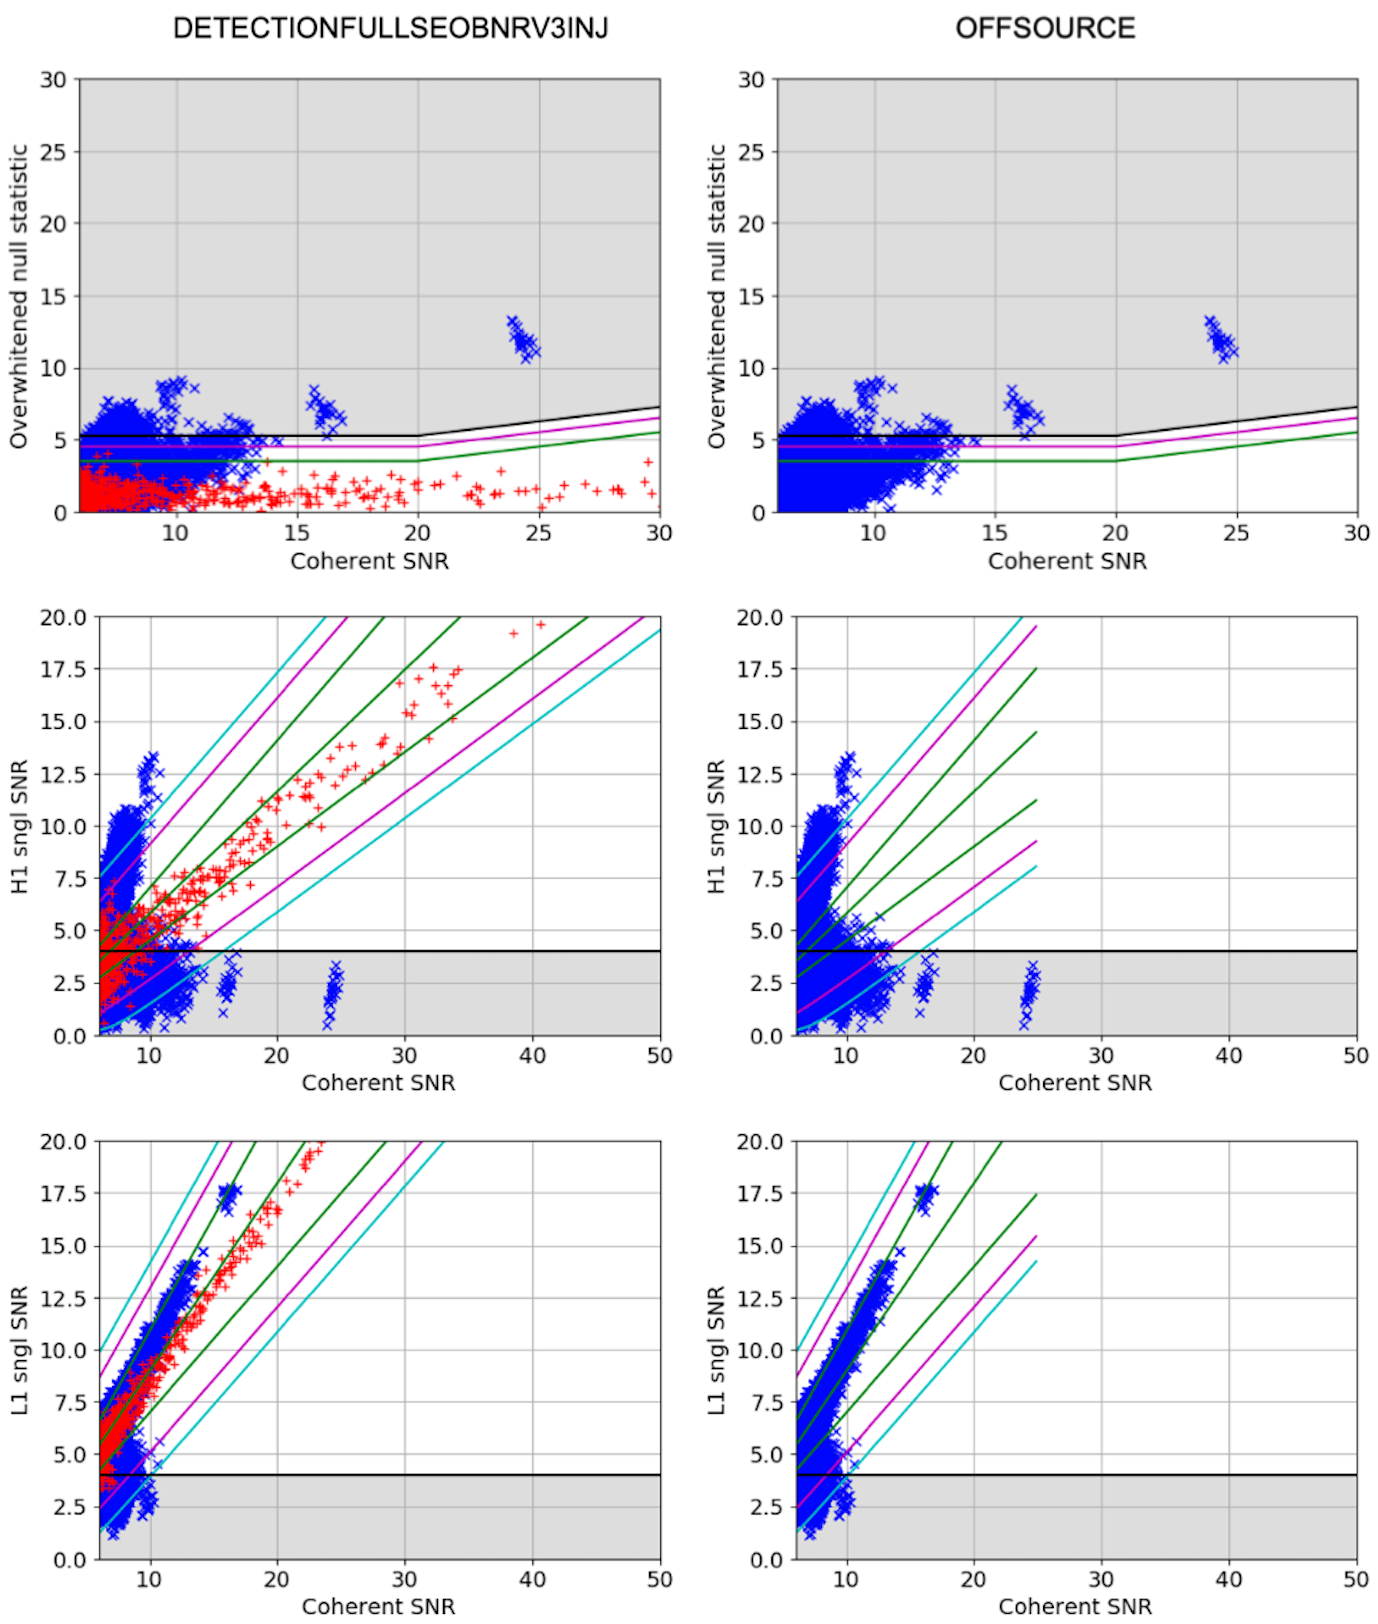
\includegraphics[width=\textwidth]{detector1}}%
          \centering
          \caption{\textbf{SNR signal consistency plots.} The two plots show the single detector SNR as a function of the coherent SNR, for H1 and L1, respectively.  Blue and red crosses represent background data and injected signals.  The expected trend for GW signals of astrophysical origin is marked by the middle, green line; the other two green lines, the two magenta lines, and the two cyan lines represent $1\sigma$, $2\sigma$, and $3\sigma$ deviations, respectively.}
          \label{fig:detector1}
        \end{figure}
	The plots in Fig.\,\ref{fig:missinj1} are an example of the results 
	one looks at to inspect the performance of the search in recover injections.
        These examples refer to the sets of precessing BNS (left) and non-precessing NSBH (right) 
	injections and display the injectioon distance as a funciton of the injection time.  
	Qualitatively, one expects the search to perform progressively worse 
	as the distances of the injections increase. 
	The distance at which the analysis begins to fail at recovering injections 
	depends on the sensitivity range of the GW detectors used in the analysis, 
	at the time of the GRB and in its directions.
	In both plots, blue crosses indicate injections that are found 
	and were more significant than any background event;
	as expected, these are found mainly nearby.
	Black crosses indicate that no trigger was found for that specific injections: 
	as expected these results dominate large distances.
	Red crosses indicate that a trigger is found in correspondence with an injection, 			
	but it was vetoed.  
	This kind of results is found in an intermediate region, 
	where the injection is weak and may be over taken by noise.  
	If a cross of this kind appears for a nearby injection, instead, 
	it generally is due to the presence of noise glitch. 
	Finally, coloured circles indicate that the injection was found, and not vetoed, 
	but was not louder than all the background triggers;  
	the circles are colour-codeded with the FAP of the recovered trigger.
	
	As discussed in Sec.\,\ref{subsec:pygrb}, the FAP is assigned to a trigger 
	by calculating the probability that a trial of the same duration as the on-source window 
	might contain a backgroung event louder than the statistics of the trigger.
        One expects circles to dominate an intermediate transition regime from 
	not confidently recovered injections (blue crosses) to not recovered injections (black crosses).  
	This transition distance is further out for more massive systems, i.e., NSBHs, 
	as the GW amplitude scales with the (chirp) mass of the source. 
	We note that missed injections can also occur within the network range.  
	Aside from the aforementioned case of glitches being present in the data, 
	this can be also be due to discrepancies between 
	the waveforms models in the template bank and the injected signals. 
	The template bank contains waveforms that do not account for precession effects, 
	and consider a maximum NS spin of $0.05$, whereas the injections sets can admit 
	precession and NS spin magnitudes up to $0.4$.
	In other words, the parameter space of the injections is larger 
	than the on strictly targetted by the template bank.
	In the case of this GRB follow up, there are 7 injections at nearby distances ($<100\,$Mpc), 
	within the BNS injection set, that warrant additional consideration: 
        2 are red crosses (missed due to vetoes) and 5 are circles (not confidently recovered).
	All of them have a high amount of precession in their dynamics and spin magnitudes greater than $0.05$ for both NSs.
	The aligned spin NSBH injection set shows a single missed injection that warrants follow up, 
	at around $-500\,$s.
	This had an antialigned BH spin of $-0.65$. 
	The injected and recovered chirp masses agree to 3 significant figures. 
	Calculating the match between the injection and the template using the same approximant returns $\sim 0.85$, 
	therefore the injection is missed due to differences between the approximant 
	used for the template (IMRPhenomD) and for the injection (SEOBNRv3).  
	These are intentially chosen to be different to account for our incomplete knowledge 
	of the \emph{exact} signal emitted by compact binaries.
        All in all, the pipeline performance in recovering the injection sets is clean.  
	Since the response to the precessing NSBH injection set is in-between the ones to the BNS and aligned NSBH injection sets,\footnote{BNSs are less massive and therefore recovered at lower distances, while aligned-spin NSBHs can be recovered up to higher distances because they lack precession effects.}
	we will show only the latter for each GRB.	

        \begin{figure}[!t]
          \noindent
          \label{missinj1}
          \centering
          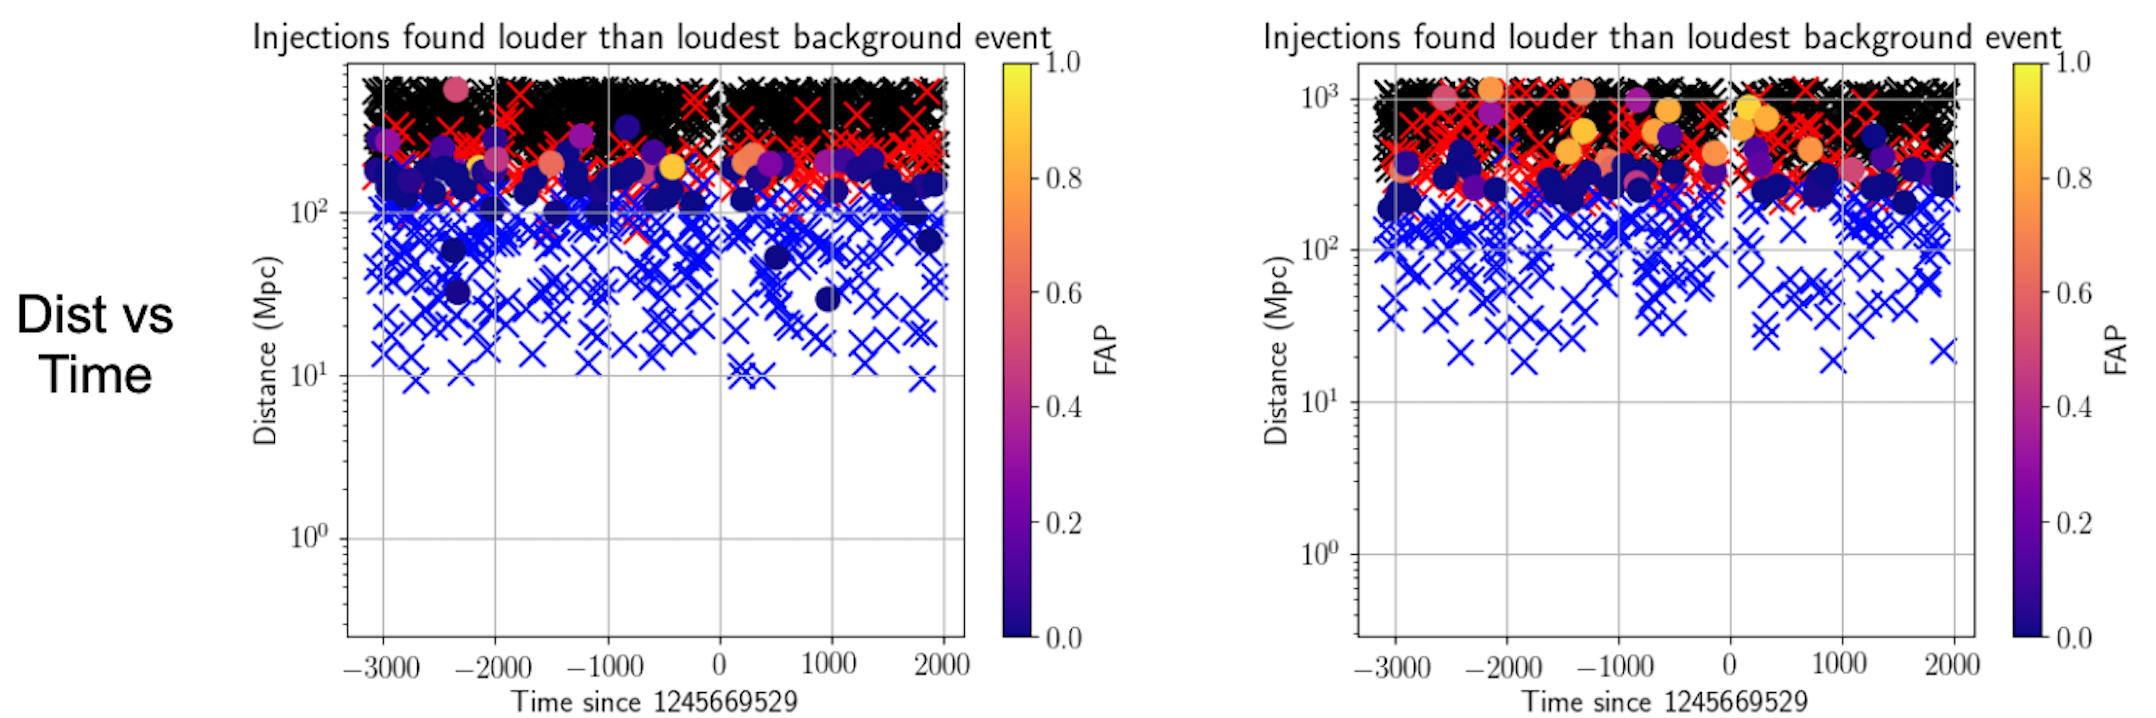
\includegraphics[width=\textwidth]{missinj1}
          \caption{\textbf{Found/missed injection plots.} Plots of the injections distance against time. Each panel represents a different injection set, with precessing BNS systems on the left and aligned-spin NSBH sources on the right. A blu cross denotes an injection that was found and that was louder than all background triggers. A coloured circle indicates that a trigger was found coincident with the injection, but it was not louder than all offsource events: its colour code is given by the FAP of the trigger.  A Red cross indicates a trigger was found coincident with the injection but it was vetoed, while a black cross indicates no trigger was found coincident with the injection.}
          \label{fig:missinj1}
        \end{figure}

	The distribution of FAPs for the background events is shown in Fig.\,\ref{fig:loudestoffsourcevent1} 
	as a function of the detection statistic, i.e., the re-weighted SNR (or ``BestNR'').
	This distribution is expected to be roughly flat up until a BestNR value of about $6$ 
	--- as triggers are kept only if $\rho_{\rm coinc} > 6$ --- 
	and to fall off linearly in this log plot from there onwards.  
	This smooth linear fall off is the behaviour of a Gaussian distribution, 
	which is what the pipeline aims at obtaining with its detection statistic.  
	The fall off should end at a BestNR  of about $8$, 
	which is the threshold for detection candidates. 
	Uneaven fall offs, or tails in the distribution are potentially signs 
	of failures in correctly handling glitches present in the background data. 
	The specific distribution in Fig.\,\ref{fig:loudestoffsourcevent1} is smooth 
	but has a small tail at the higher end of the re-weighted SNR. 
	An inspection of the list of loudest offsource events revealed that 
	this is simply a plotting artifact, as the loudest event has an upper limit on its FAP, 
	rather than a specific assigned value.  
	This upper limit coincides, of course, with the FAP of the second loudest event and hence the plotting artifact.

	Since the study of the background gave good results overall,
	the analysis proceeded by looking at the results for the on-source data.
	In order to claim the detection of a GW candidate event, this 
	must have a FAP of $\sim 10^{-4}$.  If a trigger of this kind does not emerge from the on-source window,
	a lower limit on the source distance is determined.
        This is known as the 90\% confidence exclusion distance, and is
	defined as the distance within which 90\% of the injections of a given set is recovered.
        \begin{figure}[!t]
          \noindent
          \label{loudestoffsourcevent1}
          \makebox[\textwidth]{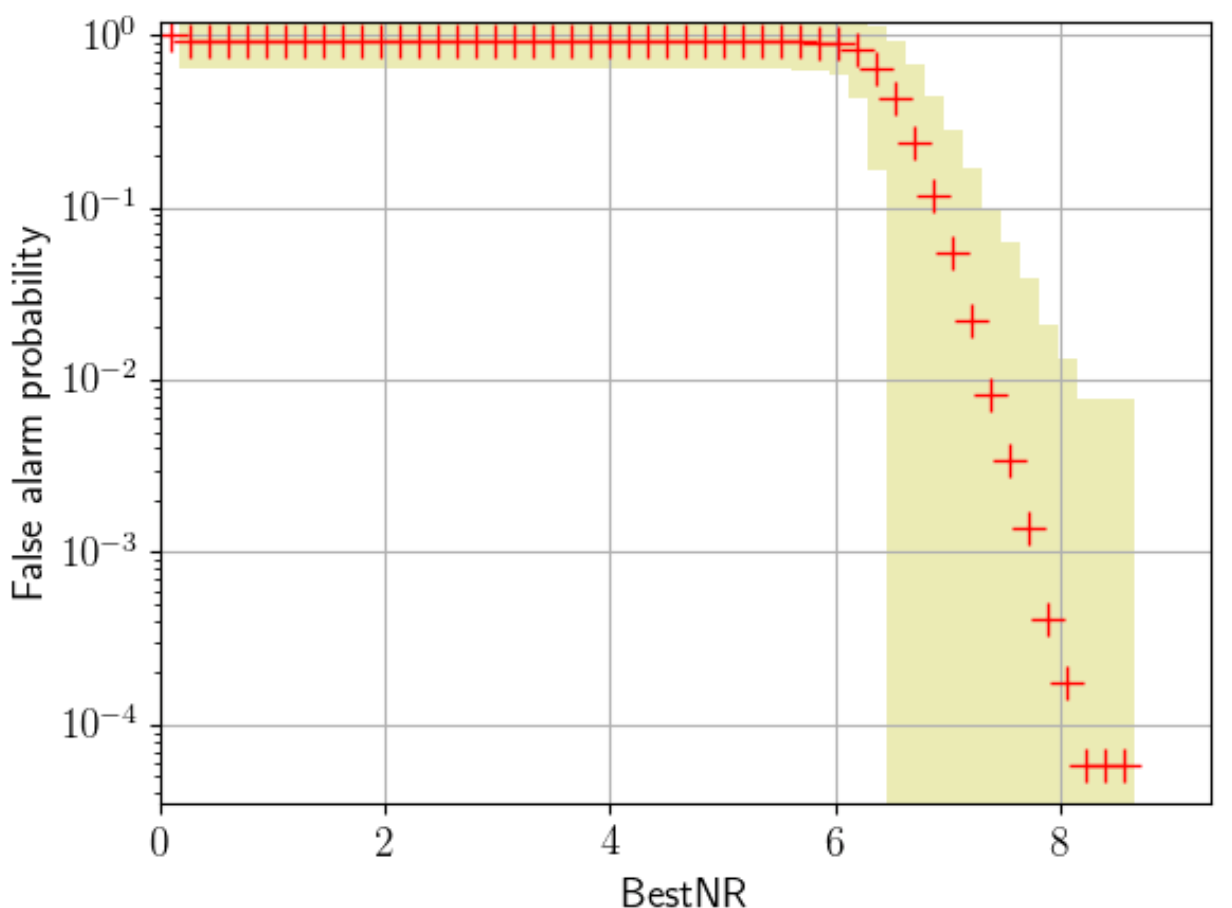
\includegraphics[scale=0.4]{loudestoffsourcevent1}}%
          \centering
          \caption{\textbf{Loudest offsource events.} Distribution of the background significance (FAP) as a function of the detection statistic (BestNR).}
          \label{fig:loudestoffsourcevent1}
        \end{figure}
	The on-source results returned a FAP of 0.481 for the loudest on source trigger, i.e., no significant event. 
	The 90\% confidence exclusion distances for the three injection sets are 115\,Mpc for BNSs, 
	139\,Mpc for precessing NSBHs, and 211 Mpc for aligned NSBHs, as reported in \cite{43}.


\subsection{GRB 190728271}
        \begin{figure}[!t]
          \noindent
          \label{scplots2_final}
          \centering
            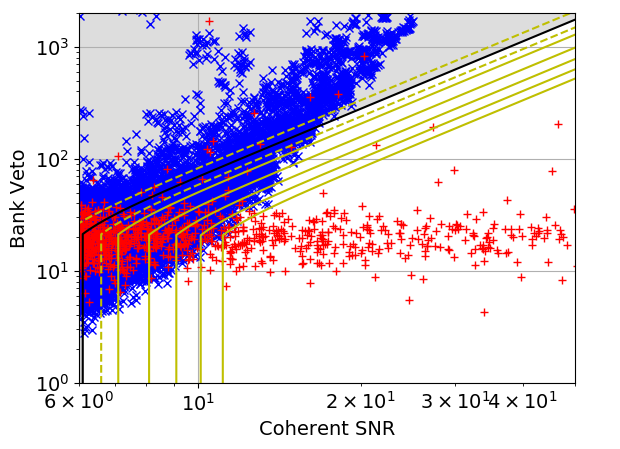
\includegraphics[width=0.67\textwidth]{GRB190728271_bank_veto_vs_snr_zoom}\\
            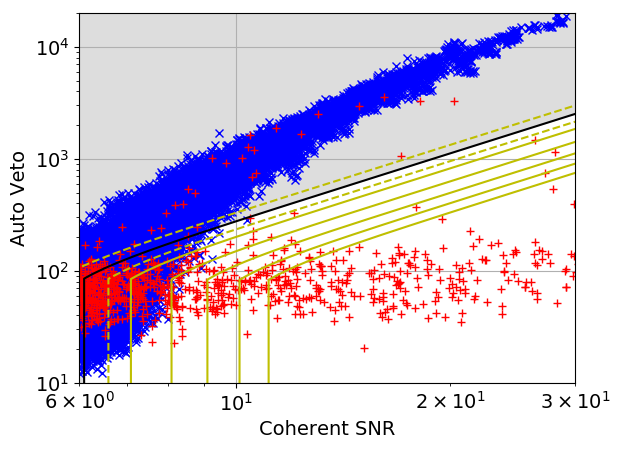
\includegraphics[width=0.67\textwidth]{GRB190728271_auto_veto_vs_snr_zoom}\\
            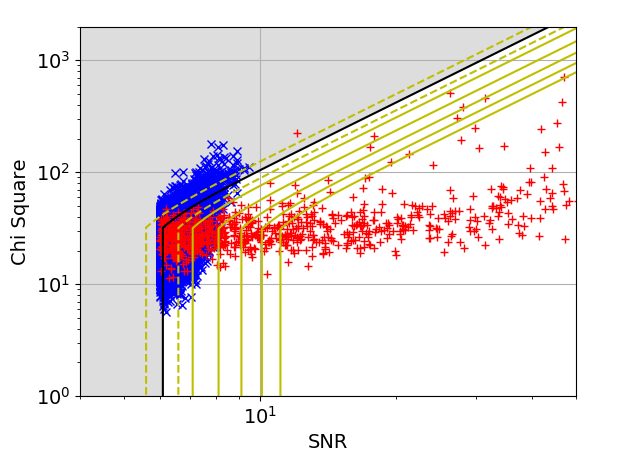
\includegraphics[width=0.67\textwidth]{GRB190728271_chi_square_vs_snr_zoom}%
          \caption{\textbf{$\chi^2$ signal consistency plots.} Same as Fig.\,\ref{fig:signalconsistencyplots1} but for GRB 190728271.}
          \label{fig:scplots2_final}
        \end{figure}

        {\it Fermi}/GBM triggered on GRB 190728271 at 06:30:36 UTC on July 28, 2019.
        The GRB was located at $RA = \ang{356.7}$, $Dec = \ang{5.4}$
        with a statistical uncertainty of $\ang{5.7}$, while the duration was $T_{90} = (0.832 \pm 0.905)\,$s.
        All three GW detectors were operating at the time of this GRB,
        and their responses in its direction were 0.271, 0.665, and 0.463 for H1, L1, and V1, respectively.

	The $\chi^2$-tests are shown in Fig.\,\ref{fig:scplots2_final}.
        In the case of the bank and auto vetoes, several injections are dragged in the vetoed area by the background.  Three auto-vetoed injections (middle panel) and a single standard-vetoed injection are not superimposed to the background triggers: these correspond to highly precessing injections and are therefore not worrisome.
        The single SNR versus coherent SNR plots (Fig.\,\ref{fig:detector2_final}) reveal that 
	the L1 has the best performance, which is in line with it having the highest antenna factor; overall these plots did not flag any issue.

        \begin{figure}[!t]
          \noindent
          \label{detector2_final}
          \centering
            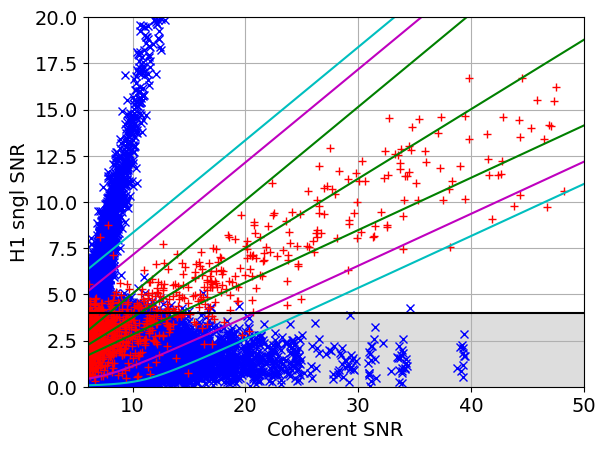
\includegraphics[width=0.64\textwidth]{GRB190728271_H1_snr_vs_snr_zoom}\\
            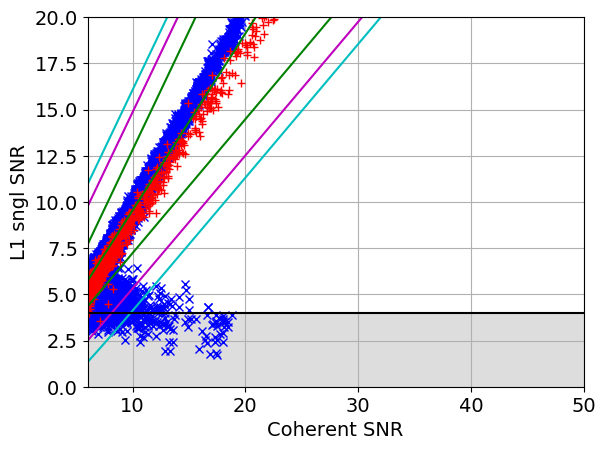
\includegraphics[width=0.64\textwidth]{GRB190728271_L1_snr_vs_snr_zoom}\\
            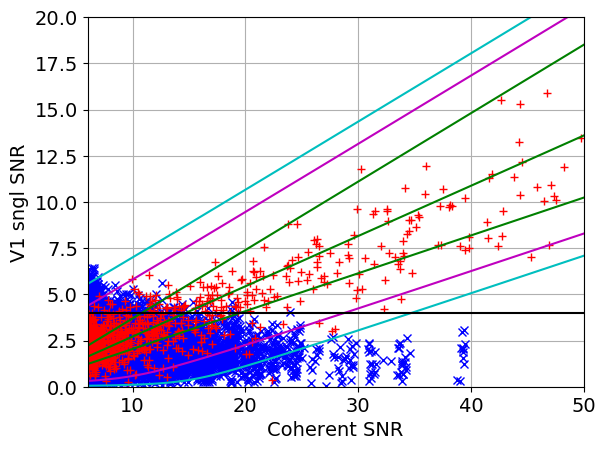
\includegraphics[width=0.64\textwidth]{GRB190728271_V1_snr_vs_snr_zoom}%
          \caption{{\bf SNR signal consistency plots.} Same as Fig.\,\ref{fig:detector1}, but for GRB 190728271 and for three detectors this time.}
          \label{fig:detector2_final}
        \end{figure}

        \begin{figure}[!t]
          \noindent
          \label{missinj2_3}
          \makebox[\textwidth]{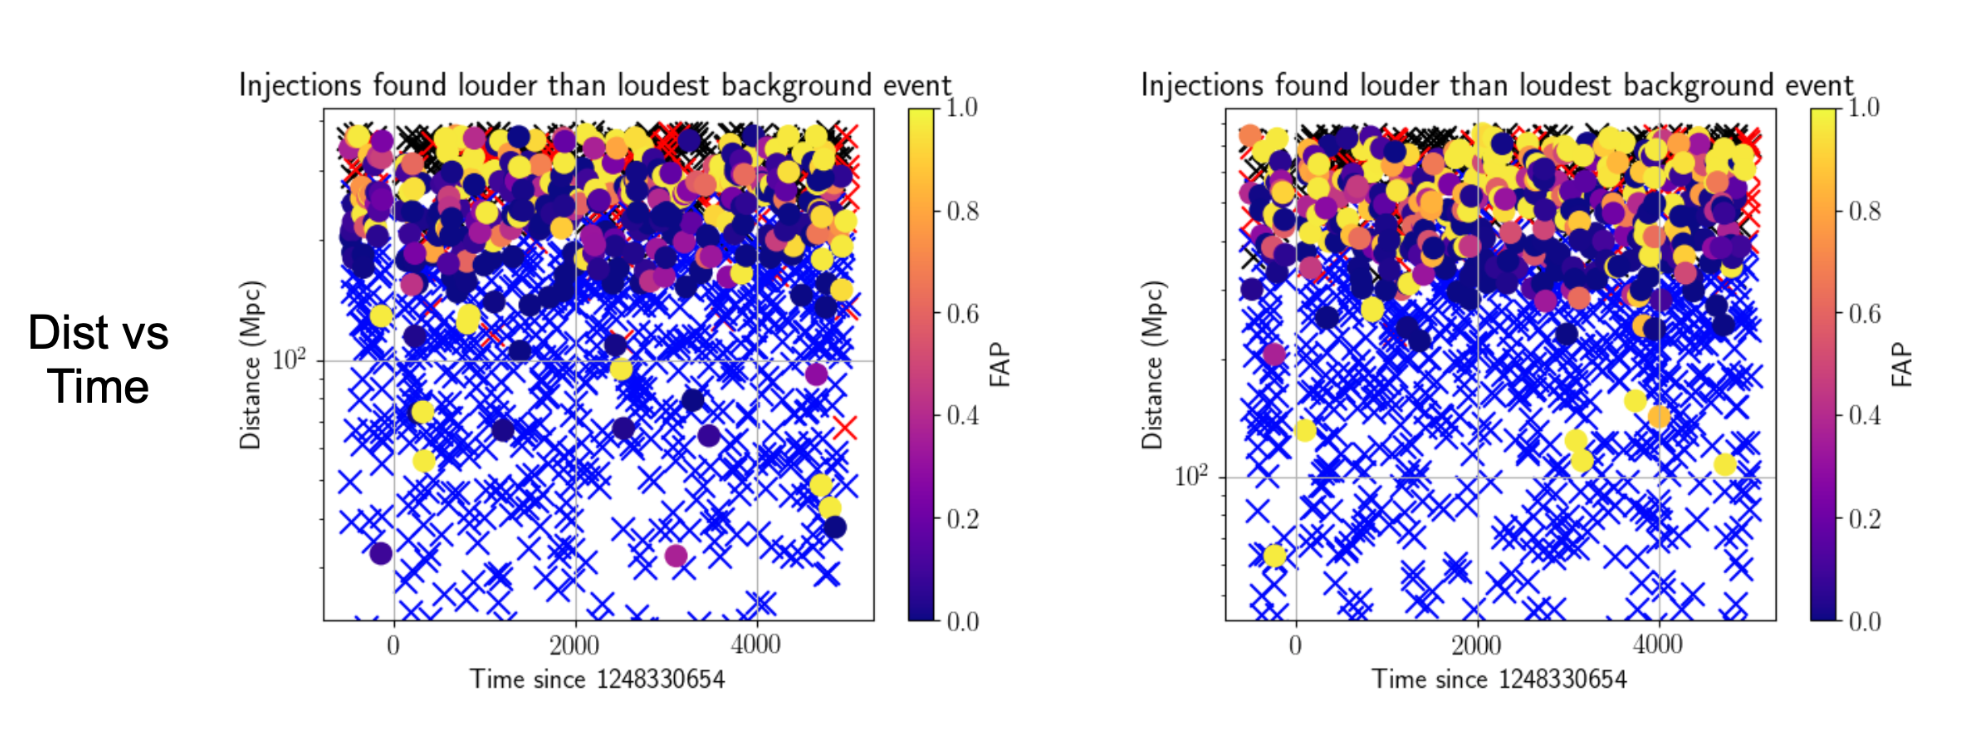
\includegraphics[width=\textwidth]{missinj2_3}}%
          \centering
          \caption{\textbf{Found/missed injection plots.} Same as Fig.\,\ref{fig:missinj1} but for GRB 190728271.}
          \label{fig:missinj2_3}
        \end{figure}

        Finally, Fig.\,\ref{fig:missinj2_3} shows the result of the injection recovery study.  Twenty nearby BNS injections were found not to be recovered confidently.
        All of them have at least one spin magnitude greater than 0.05, with moderate to high precession. 
	Further, two injections were missed due to high $\chi^2$ and NullSNR values, caused by a glitch in the L1 data.
	A high NS spin magnitude ($\sim 0.3$) also caused a single nearby NSBH injections to not be recovered as louder than all the background events.
        As for GRB 190627A, this background analysis gave overall good results,
	and the on-source data results were investigated.
	The loudest onsource event was given a FAP of 0.513, so it is not of astrophysical origin.  The $90\%$ confidence exclusion distances for the on-source window are 160\,Mpc, 204\,Mpc and 272\,Mpc for the BNS, the precessing and aligned NSBH, respectively, as reported in \cite{43}.

\subsection{GRB 190425089}
        GRB 190425089 was observed at 02:07:43 on April 25, 2019 by the Swift satellite,
        with a sky position of $RA=\ang{126.5}$ and $Dec=\ang{-58.1}$.

	Initially the follow-up analysis of this GRB was carried out using data from all three available GW detectors.
        However, the antenna factor for V1 (0.47) in this case was much lower than those of H1 (0.852) and L1 (0.923).
        This inhomogeneous antenna response emerges in an evident manner in the  single detector SNR versus coherent SNR plots (Fig.\,\ref{fig:detector3}):
        while the distribution of injections looks clean for H1 and L1, with the exception of a single one outside the $3 \sigma$ region for H1,
        the V1 plot does not show the expected trend for astrophysical signals.
        \begin{figure}[!t]
          \noindent
          \label{detector3}
          \makebox[\textwidth]{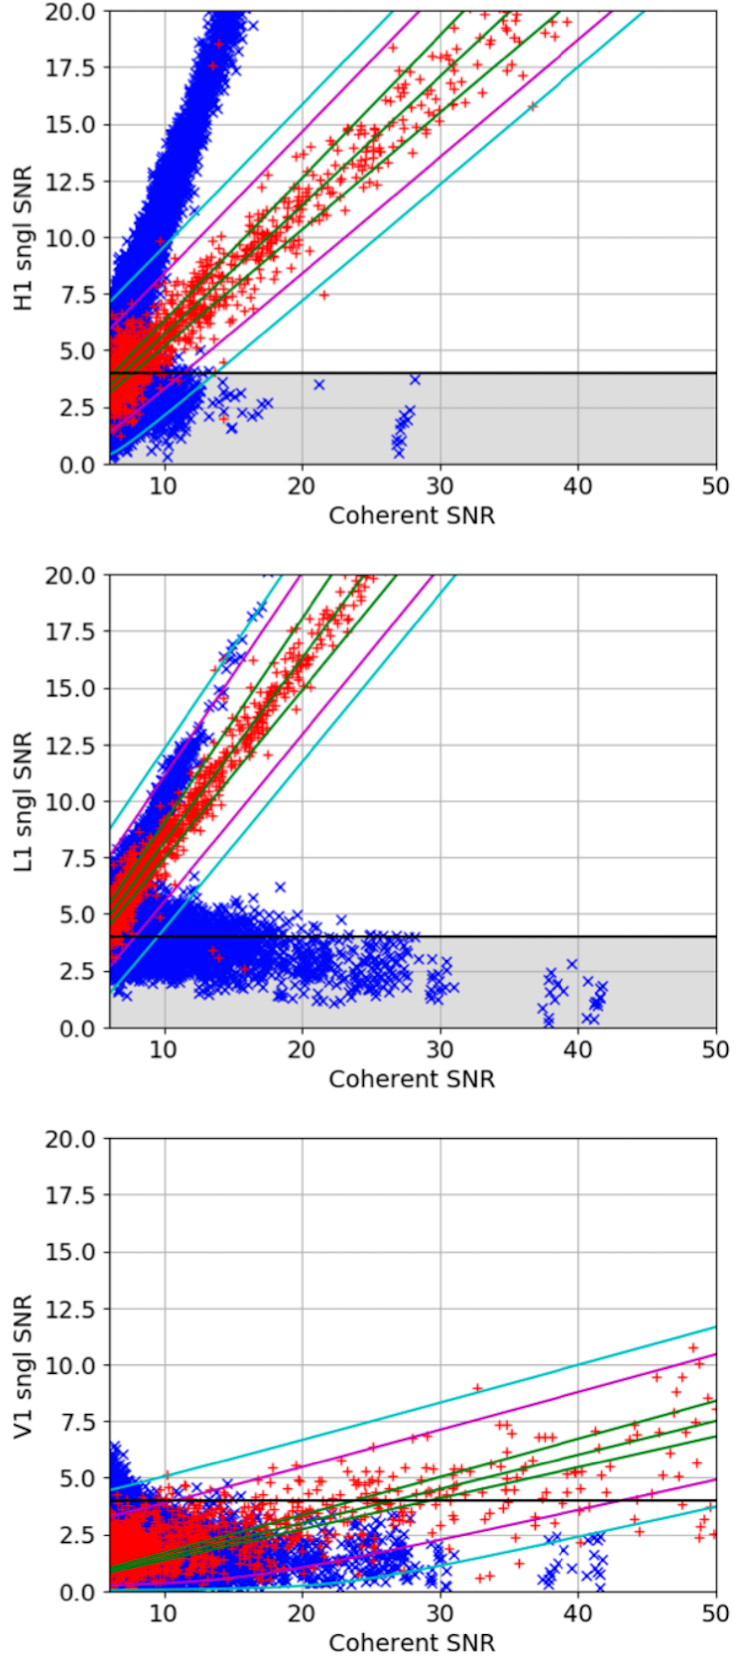
\includegraphics[width=0.66\textwidth]{detector3}}%
          \centering
          \caption{{\bf SNR signal consistency plots.} Same as Fig.\,\ref{fig:detector1} but for GRB 190425089.}
          \label{fig:detector3}
        \end{figure}

 	Therefore, the production analysis was conducted without considering the V1 data.
	The results of the $\chi^2$-tests are shown in Fig.\,\ref{fig:signalconsistencyplots3_final}:
       	a few injections that overlap with glitches in the data are dragged into the vetoed area of the bank and auto veto tests, while a single injection is vetoed by the $\chi^2$-test.  This corresponded to a BNS with spin $\sim 0.4$ for one of its two components and is therefore not worrisome.  In summary, the performance of the pipeline is adequate.

        \begin{figure}[!t]
          \noindent
          \label{signalconsistencyplots3_final}
          \makebox[\textwidth]{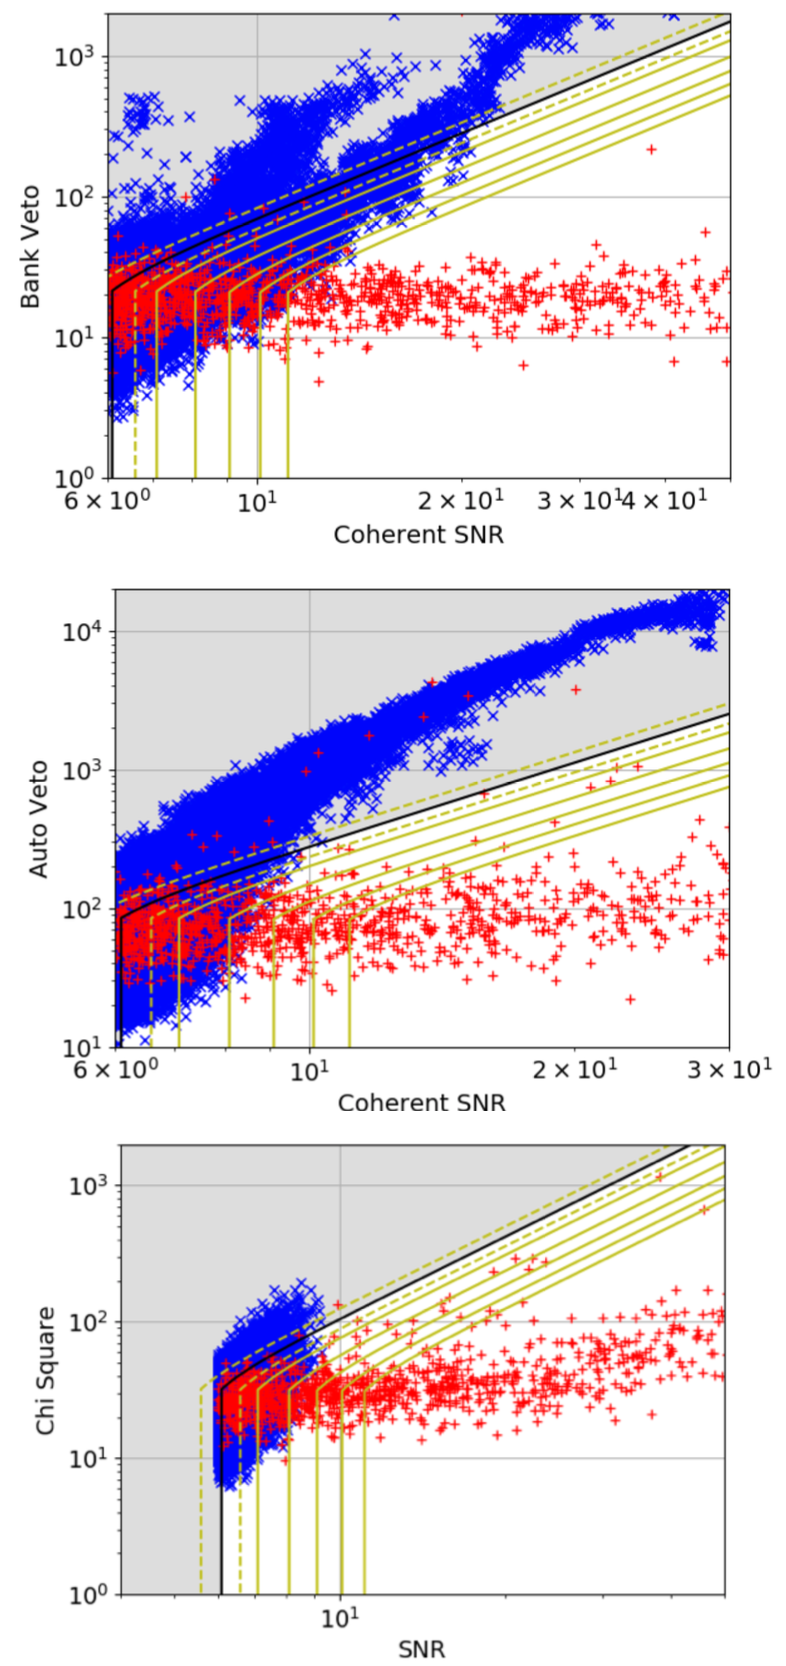
\includegraphics[width=0.69\textwidth]{signalconsistencyplots3_final}}%
          \centering
          \caption{\textbf{$\chi^2$ signal consistency plots.} Same as Fig.\,\ref{fig:signalconsistencyplots1} but for GRB 190425089.}
          \label{fig:signalconsistencyplots3_final}
        \end{figure}

	The plots of the of the single SNR versus coherent SNR reported in Fig.\,\ref{fig:detector3_final} show that both H1 and L1
	follow the expected astrophysical trend overall, with just one injection falling out the 3$\sigma$ deviation in H1.  This corresponds to a BNS with highly spinning and precessing NSs and is therefore not surprising.
        \begin{figure}[!t]
          \noindent
          \label{detector3_final}
          \makebox[\textwidth]{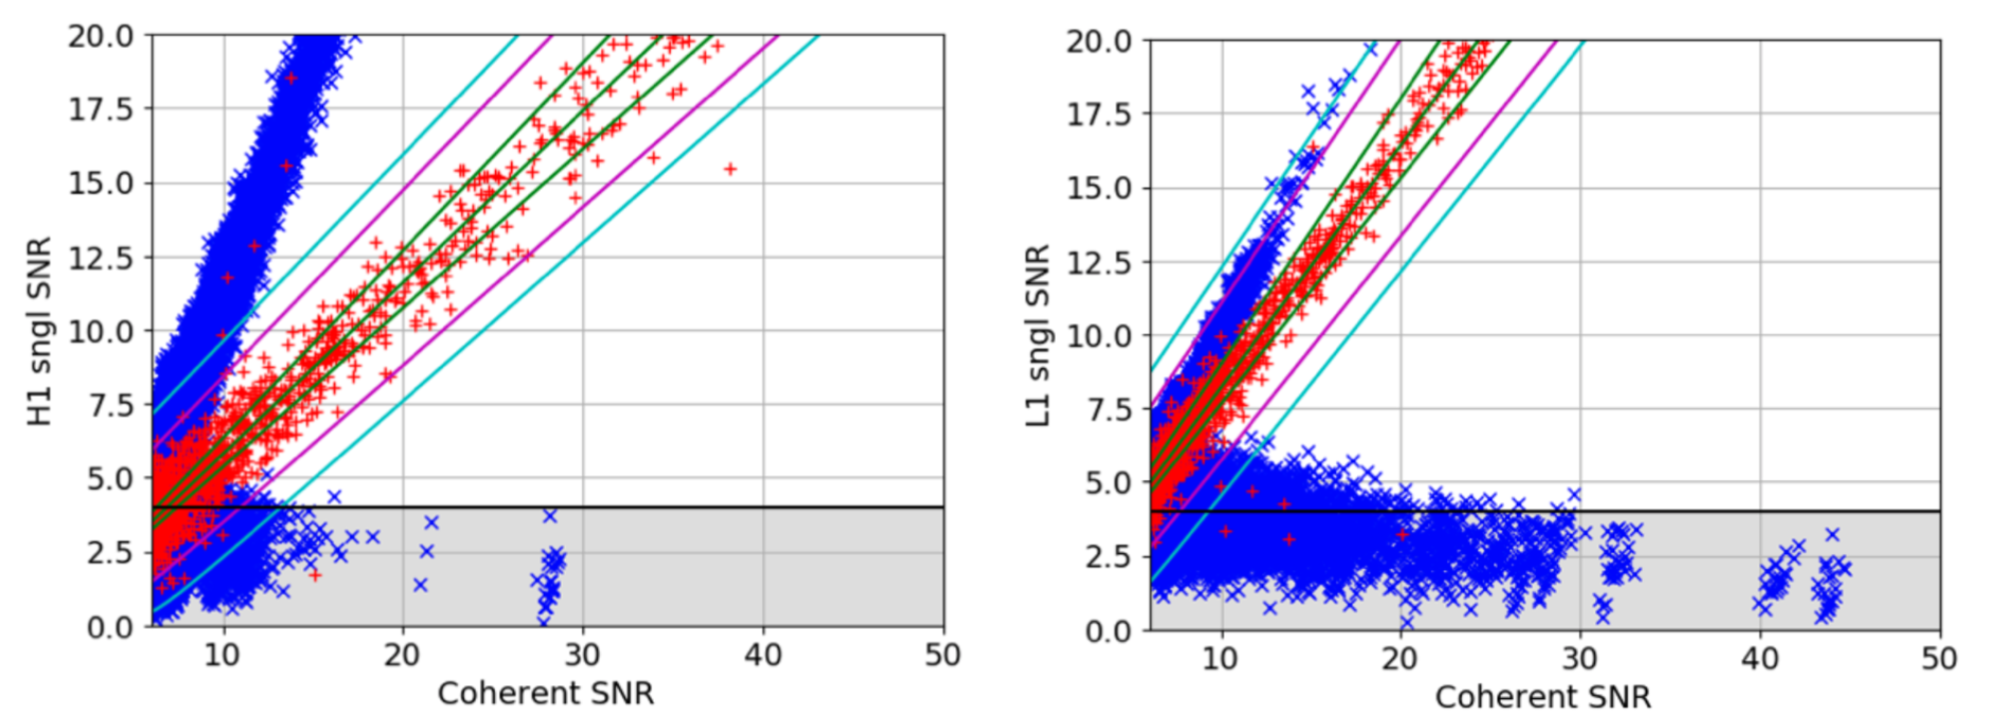
\includegraphics[width=\textwidth]{detector3_final}}%
          \centering
          \caption{\textbf{SNR consistency plots.} Same as Fig.\,\ref{fig:detector1} but for GRB 190425089. These plot show the re-analysis of  GRB 190425089 without V1.}
          \label{fig:detector3_final}
        \end{figure}
	
        Finally, the found and missed injections are reported in the panels of Fig.\,\ref{fig:missinj3_5}.  An inspection of the aligned spin NSBH missed injections shows that they overlap with glithces in one of the two LIGO interferometers, while the nearby injections that are not recovered as louder than all the background have a NS with spin magnitude above $0.05$.
        Similar considerations apply to the BNS injection set.
        \begin{figure}[!t]
          \noindent
          \label{missinj3_5}
          \makebox[\textwidth]{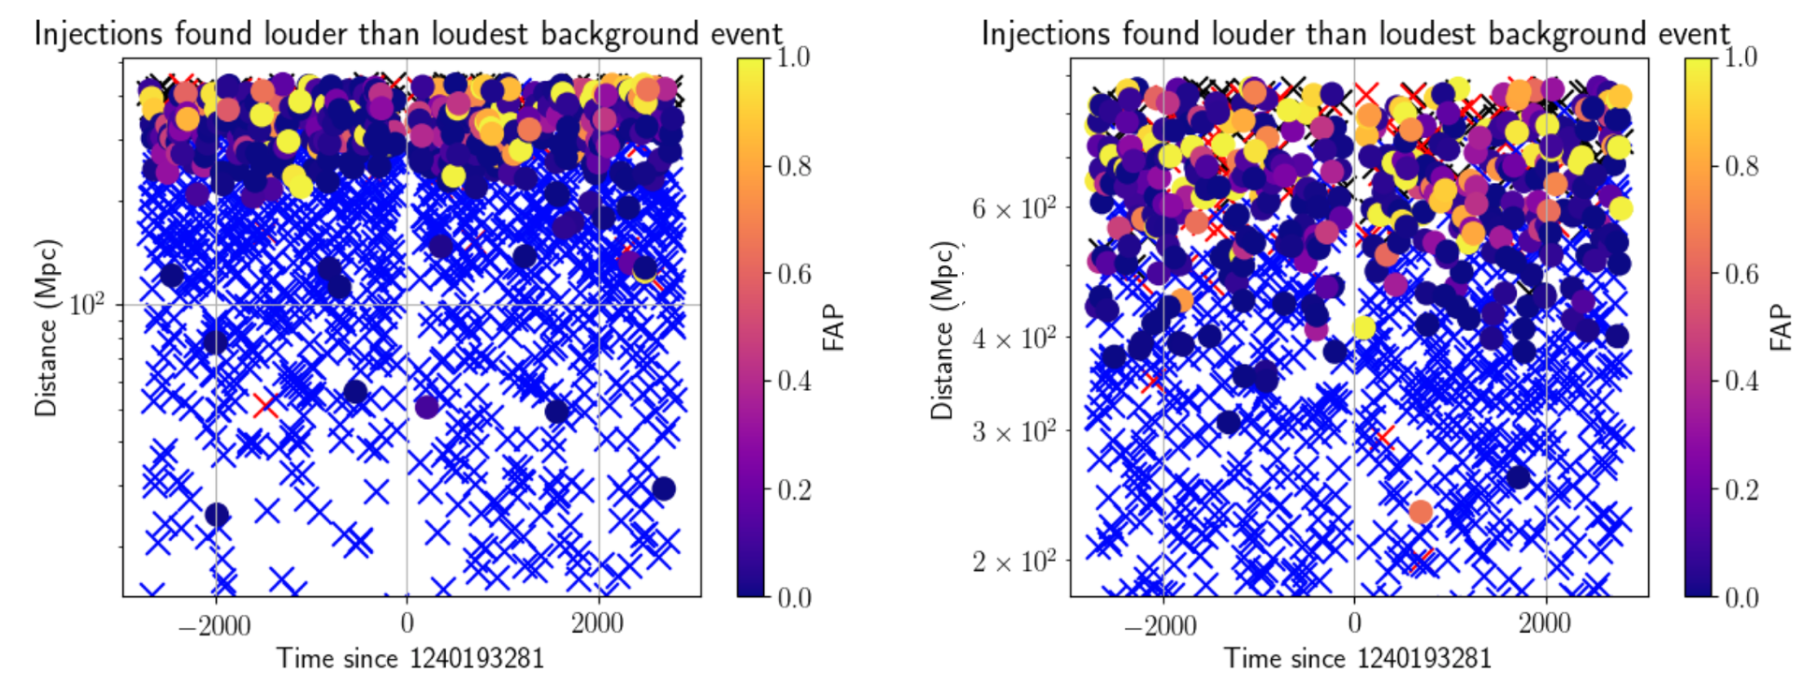
\includegraphics[width=\textwidth]{missinj3_5}}%
          \centering
          \caption{\textbf{Found/missed injections.} Same as Fig.\,\ref{fig:missinj1} but for GRB 190425089.}
          \label{fig:missinj3_5}
        \end{figure}
	Overall the background analysis gave acceptable results
	and the on-source data results were investigated: 
	the loudest event had a FAP of 0.075 which is not significant astrophysically.  The 90\% confidence exclusion distance for BNS, generic spin NSBH and aligned spin NSBH sources were found to be 204\,Mpc, 247\,Mpc and 440\,Mpc, respectively, as reported in \cite{43}.



\section{Coincident Analysis of a Chunk of O3b Data}
\label{sec:pycbc00}
	The {\texttt{PyCBC}} coincident search targets GWs from CBCs with a total mass of $2$--$500\,M_\odot$,
        and with maximal dimensionless spin parameters of 0.998 and 0.05 for BH s and NSs, respectively,
        providing a measure of their statistical significance.
        This analysis filters each single detector data stream with a template bank (Sec.\,\ref{subsec:mfcbc}),
        and calculates the coincident SNR for each combination of detectors (Sec.\,\ref{subsec:coincident}).

	Data from an observing run are split into \emph{chunks},
	stretches of data identified by their GPS start and stop times and
	determined operationally as follows.
	The chunk start time is when at least one detector is in observing mode;
	after five days of coincident time between all the detectors in the network are accumulated,
	the chunk ends as soon as the same starting network configuration is available.
        This time period is long enough to build an extended enough background, 
	but short enough that the sensitivity of the instruments does not vary too much. 
	Start and end times require to be padded on both ends with 8\,s of extra data 	
	to ensure a correct behaviour of the high/low pass filters.

        I analysed a chunk of data from the second half of the third observing run (O3b).  
	This chunk ran from 01:31:32 UTC on December 20, 2019 to 15:40:36 UTC on December 28, 2019.
	Since the detector outputs voltages at the anti-symmetric port, 
	data calibration is necessary to convert from units of volts to units of strain.
	The data immediately available is denoted by the label ``C00''  
	and it has higher uncertainties in the function used to convert from voltage to strain, 
	with respect to final calibration data versions that require longer times to be produced, as
        numerous data quality checks and calibration studies are carried out.
        While this process takes place, C00 data is analyzed to provide preliminary results.
	The data I processed was C00 data and came from the two LIGO detectors.
	It contained 8.59 days of raw calibrated data,
        of which 6.235 days (72\%) constituted coincident time.
        Since the LIGO-Virgo Collaboration has not published O3b results yet, 
	I will not disclose any of the foreground, but I will limit the discussion to the analysis of the background.

        \begin{figure}[!t]
          \noindent
          \label{asd}
          \makebox[\textwidth]{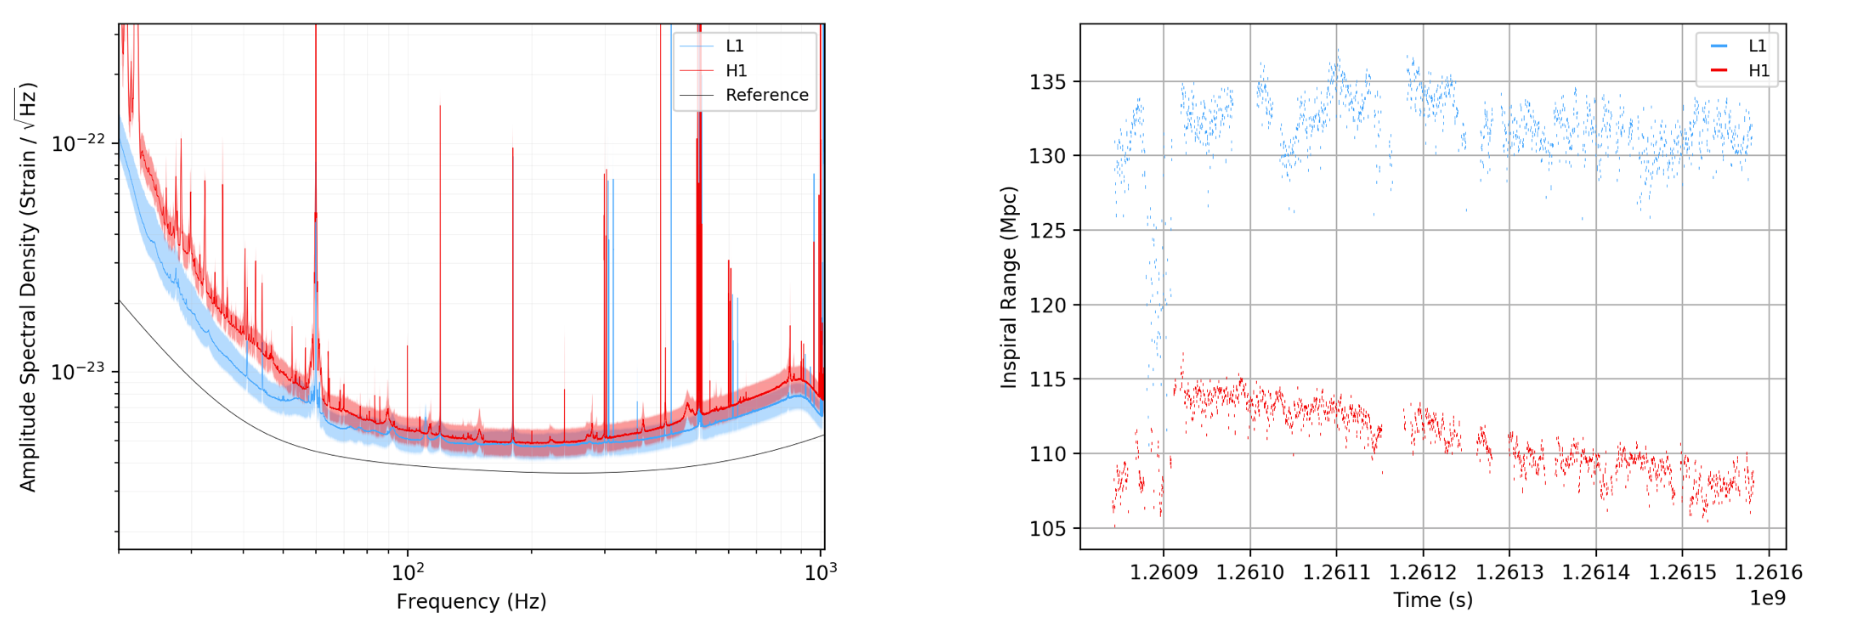
\includegraphics[width=\textwidth]{asd}}%
          \centering
          \caption{(\textit{Left}) Amplitude spectral density as a function of frequency for the Hanford (H1) and Livingston (L1) detectors. The grey line labelled as ``Reference'' is the design sensitivity for the Advanced LIGO detectors. (\textit{Right}) Inspiral range as a function of time for a binary neutron star with $m1 = m2 = 1.4 M_\odot$ at a single detector SNR $\rho = 8$.}
          \label{fig:asd}
        \end{figure}
        \begin{figure}[!t]
          \noindent
          \label{snrhistogram}
          \makebox[\textwidth]{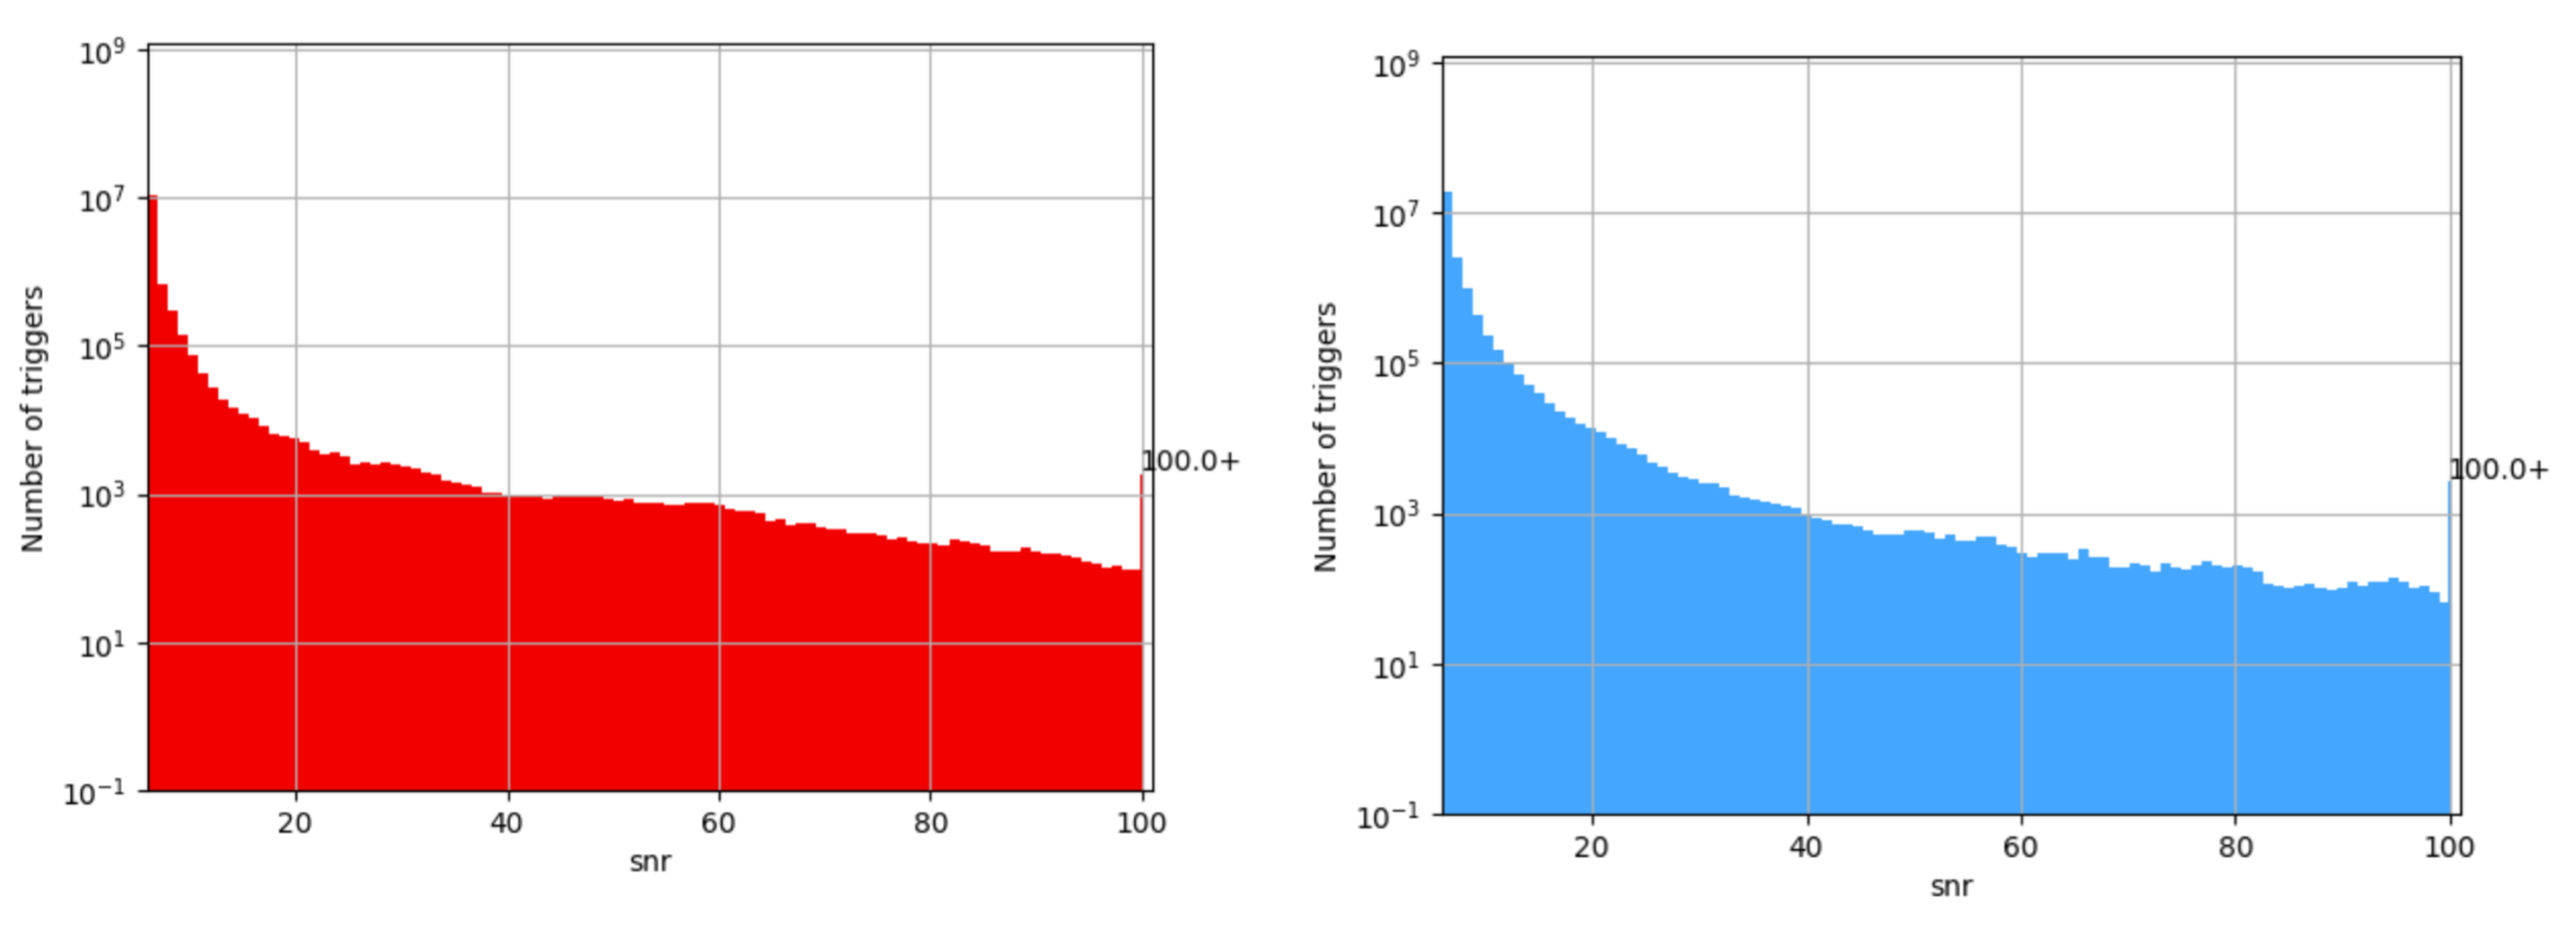
\includegraphics[width=\textwidth]{snrhistogram}}%
          \centering
          \caption{Histograms of the re-weighted SNR of the background events for the Hanford detector (\textit{left}) and the Livingston detector (\textit{right}).}
          \label{fig:snrhistogram}
        \end{figure}

	One of the goals of the offline analysis is to perform basic sanity checks 
	by identifying problematic noise transients in the data or analysis issues.
	Long time scale non-stationarity in the data can be obtained from the amplitude spectral density 
	and the inspiral range measured in the search, shown in Fig.\,\ref{fig:asd}.
	The detector sensitivity can be affected by times of troubling data, 
	and a symptom of this is embodied  by  an abrupt inspiral range drop.
	Short transients manifest themselves as high re-weighted SNR triggers in the background distribution. 
	To identify these glitches and subsequently  assess if they can be vetoed before the coincidence test, 
	the histograms of the background SNR and re-weighted SNR (see example in Fig.\,\ref{fig:snrhistogram}) 
	may be inspected to look for an excess of noise transients in the data.
	Accordingly, the loudest background triggers are followed up individually, 
	as described in the next section.
	A data quality flag is applied to those times when known instrumental noise transients are found, 
	indicating that they should be vetoed by the analysis. 
	With the new data quality information, the search analysis is then repeated.  
        For the chunk under investigation here, these preliminary analyses did not reveal any particular issue.

        \begin{figure}[t]
          \noindent
          \label{sens_vt}
          \makebox[\textwidth]{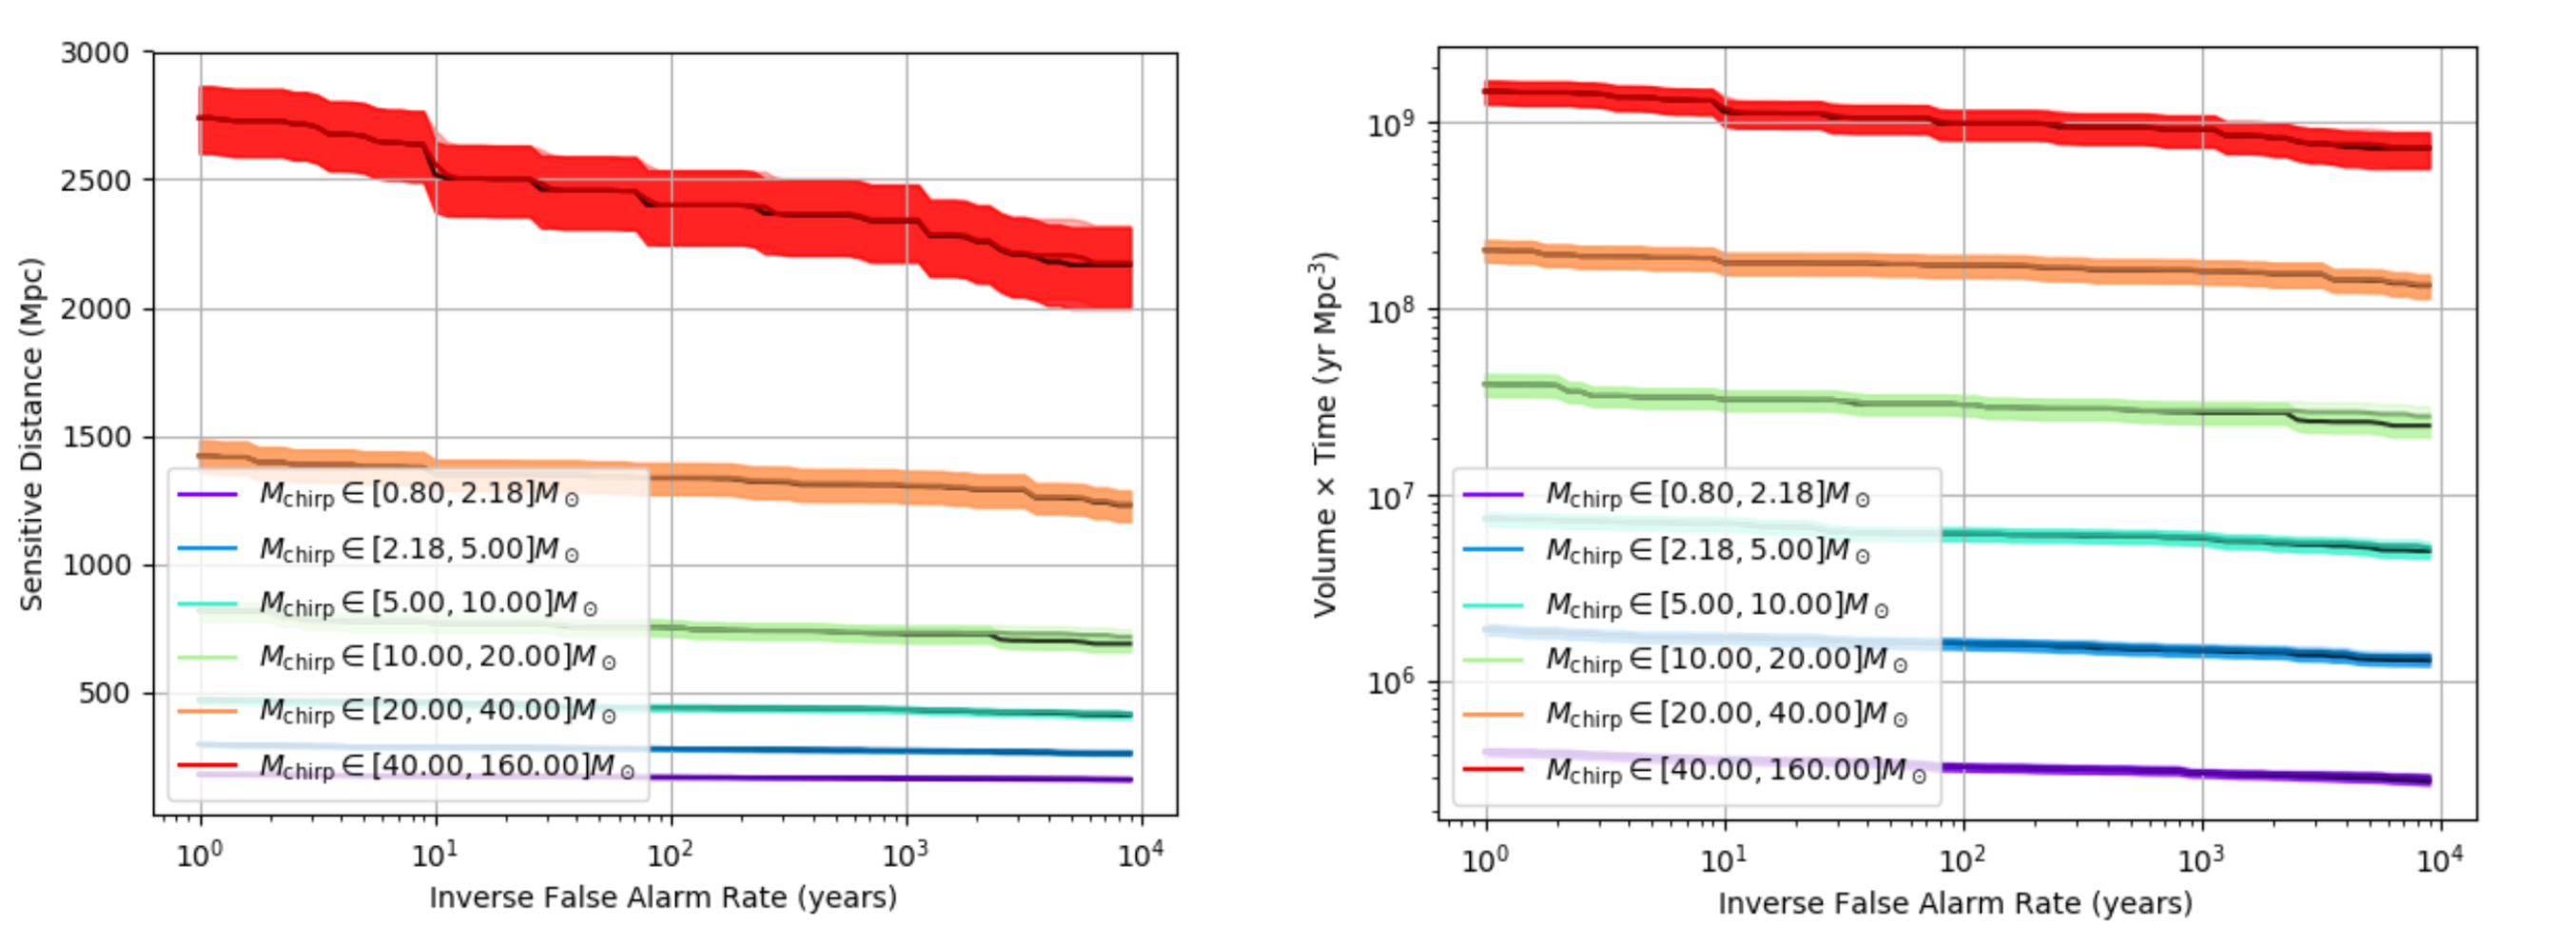
\includegraphics[width=\textwidth]{sens_vt}}%
          \centering
          \caption{Sensitive distance (\textit{left}) and sensitive volume $\times$ time (\textit{right}) of the {\texttt{PyCBC}} search as functions of the inverse false-alarm rate for six chirp-mass bins. The sensitivity is estimated from the missed and found injections added to the data. Darker lines represent the significance without including injections in their own background, while lighter lines include each injection individually in the background estimation for that signal.}
          \label{fig:sens_vt}
        \end{figure}

	The analysis carried out must assign a statistical significance to candidate events.
        The data is therefore used to study the background by looking at the effects of a time-shifted analysis in which, 
	as stated in Sec.\,\ref{subsec:far}, the data streams of the instruments are repeatedly shifted by a constant time offset with respect to each other. 
	Typically, the time-shift used to construct HL backgrouns is 0.1\,s.
	The time-shifted analysis candidates, i.e., coincidences contained in this artificial data, 
	are not candidates of astrophysical origin, as the time shift is greater than the light travel time between detectors.
	In the two-detector configuration, applying time shifts is straightforward as shifting one detector 
	is entirely equivalent to shifting the other detector in the other direction. 
        At the same time, this background data is used to assess the performance of the pipeline in terms of its sensitivity, 
	ability to discriminate between signal and background, ability to predict the background model, etc. 
	Like for most other detection pipelines, this is done by using a large number of simulated signals (injections) that are added to the background data in software and recovered.
 	The fraction of simulated signals that the pipeline is able to identify at a given false-alarm rate gives a measure of the search sensitive volume.
	The results of this processes are shown in  Fig.\,\ref{fig:sens_vt}: 
	the injections are grouped into chirp mass bins, since the GW amplitude scales with the chirp mass,
	and the sensitivity is determined for each bin.
	The sensitive volumes multiplied by the analysis time are also shown to quantify the amount of time removed by data quality vetoes.

        The individual follow up of loud single-detector noise triggers (``singles'') and missed injections is 
	described in the next two sections; the outcome of these invastigations can lead to a re-analysis of the data whenever an unexpected behaviour of the pipeline is identified. 


\subsection{Loudest Singles}
	After the data from each detector is individually match filtered,
	triggers are generated by thresholding and clustering the
        single-interferometer SNR timeseries.
        Whenever the threshold of 5.5 is exceeded,
        the pipeline produces a single-detector trigger associated with the detector,
        the parameters of the template, and the coalescence time.
	A list of triggers is generated for the detectors present in the network --- namely, two for the specific analysis discussed herein --- and divided into bins according to the template-length.  The bins contain:
	\begin{enumerate}
        \item triggers with template duration $<0.6\,$s; 
        \item triggers with template duration between 0.6\,s and 4.0\,s, and
        \item the remaining triggers, with template duration greater
          than $4.0\,$s.
        \end{enumerate}
        The first bin is likelier to catch noise transients, given its templates are short and can latch onto noise transients more easily.
	Since single detector triggers may also be caused by noise transients,
	other than by GW signals, 
	it is crucial to identify the nature of the origin of the loudest non-coincident triggers in both detectors.
        Strain spectrograms (``heat maps'' in the time-frequency plane) are generated around the times of the loudest triggers with this purpose.
        Further, the triggers are subject to a chi-squared test (Sec.\,\ref{subsec:chi_square_test}).

%H1_Loudest
        \begin{figure}[t]
          \noindent
          \label{glitch}
          \makebox[\textwidth]{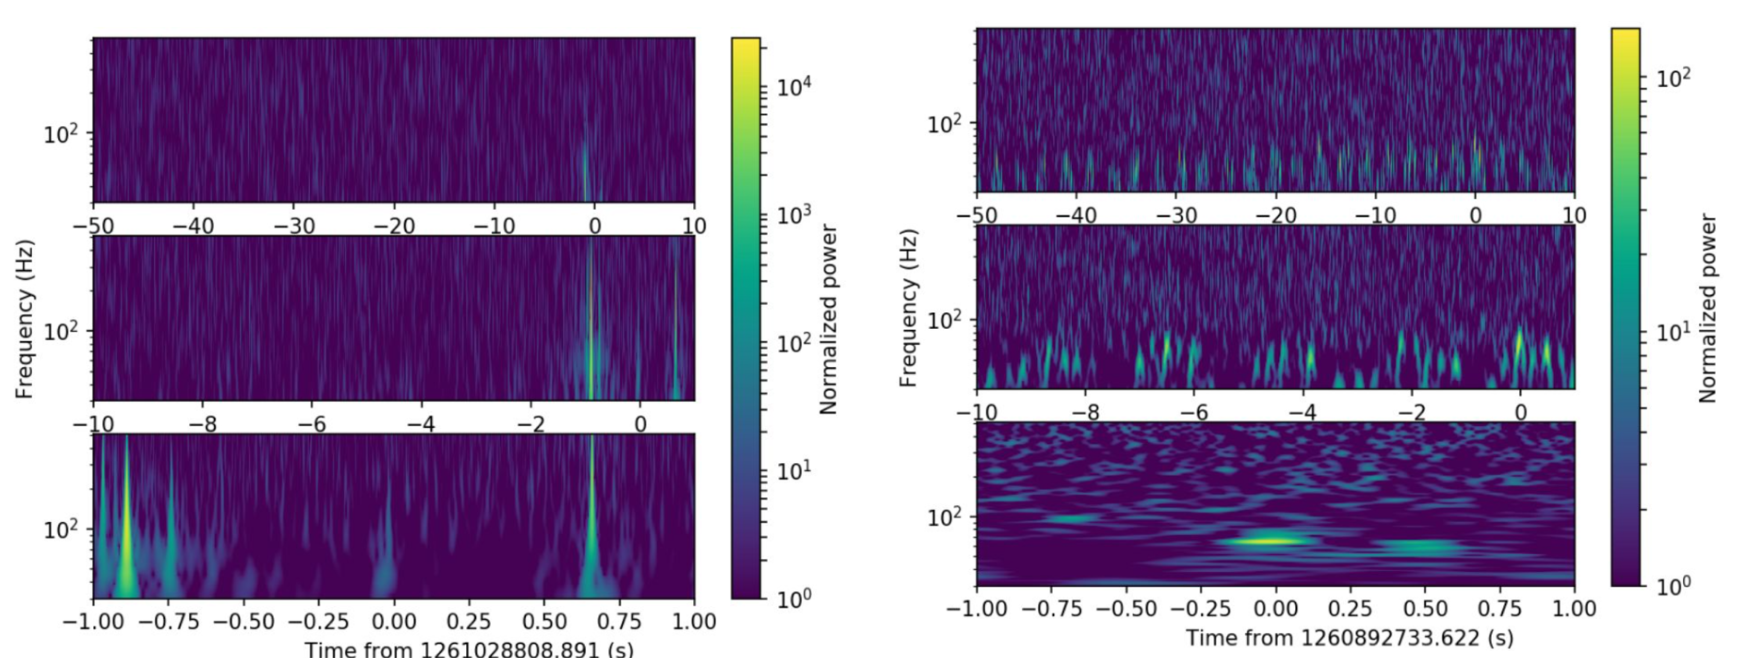
\includegraphics[scale=0.45]{glitch}}%
          \centering
          \caption{{\bf Blip and comb-like glitches.} Time-frequency spectrogram of $2\,$s around a loud blip glitch in H1 (left) and for a comb-like glitch in L1 (right).  The horizontal axis shows how long the glitch lasts and the vertical axis shows its frequency content, i.e., where it ``rings'' the template.  The colourcode represent the loudness of the glitch.}
          \label{fig:glitches}
        \end{figure}

	When looking at the loudest --- i.e., greater than 8 --- H1-only triggers in my dataset,
	it was possible to identify various kinds of glitches as the cause of the high SNR value.
	In the majority of cases, these fell in proximity of loud glitches that had been gated out (Sec.\,\ref{sec:ranking}) during the analysis.
	By inspecting their spectrograms, three loud single-detector triggers were identified as {\it blip}-like glitches,
	short-duration glitches with a symmetric ``teardrop'' shape that have been witnessed to happen randomly in time in GW detectors.
	The left panel in Fig.\,\ref{fig:glitches} shows one of these loud blip glitches in H1, with a few fainter blip glitches around it on a $\sim 1\,$s timescale.
        Glitches of this kind are particularly harmful to the search since they survive the $\chi^2$-test: 
	Fig.\,\ref{fig:chisquared} shows the behaviour of the reduced $\chi^2$ time-series, which perfectly mimics the beahviour of a real signal.
	Besides short blip glitches, five \emph{scratchy blips} spanning a duration of $\gtrsim 2\,$s were identified in the second bin.
	As expected, the third bin, with its templates containing several cycles, was the quietest: the majority of the triggers it cointained looked like random noise barely above threshold, and 
	lacking any distinctive features in the spectrograms.

	 \begin{figure}[t]
          \noindent
          \label{chisquared}
          \makebox[\textwidth]{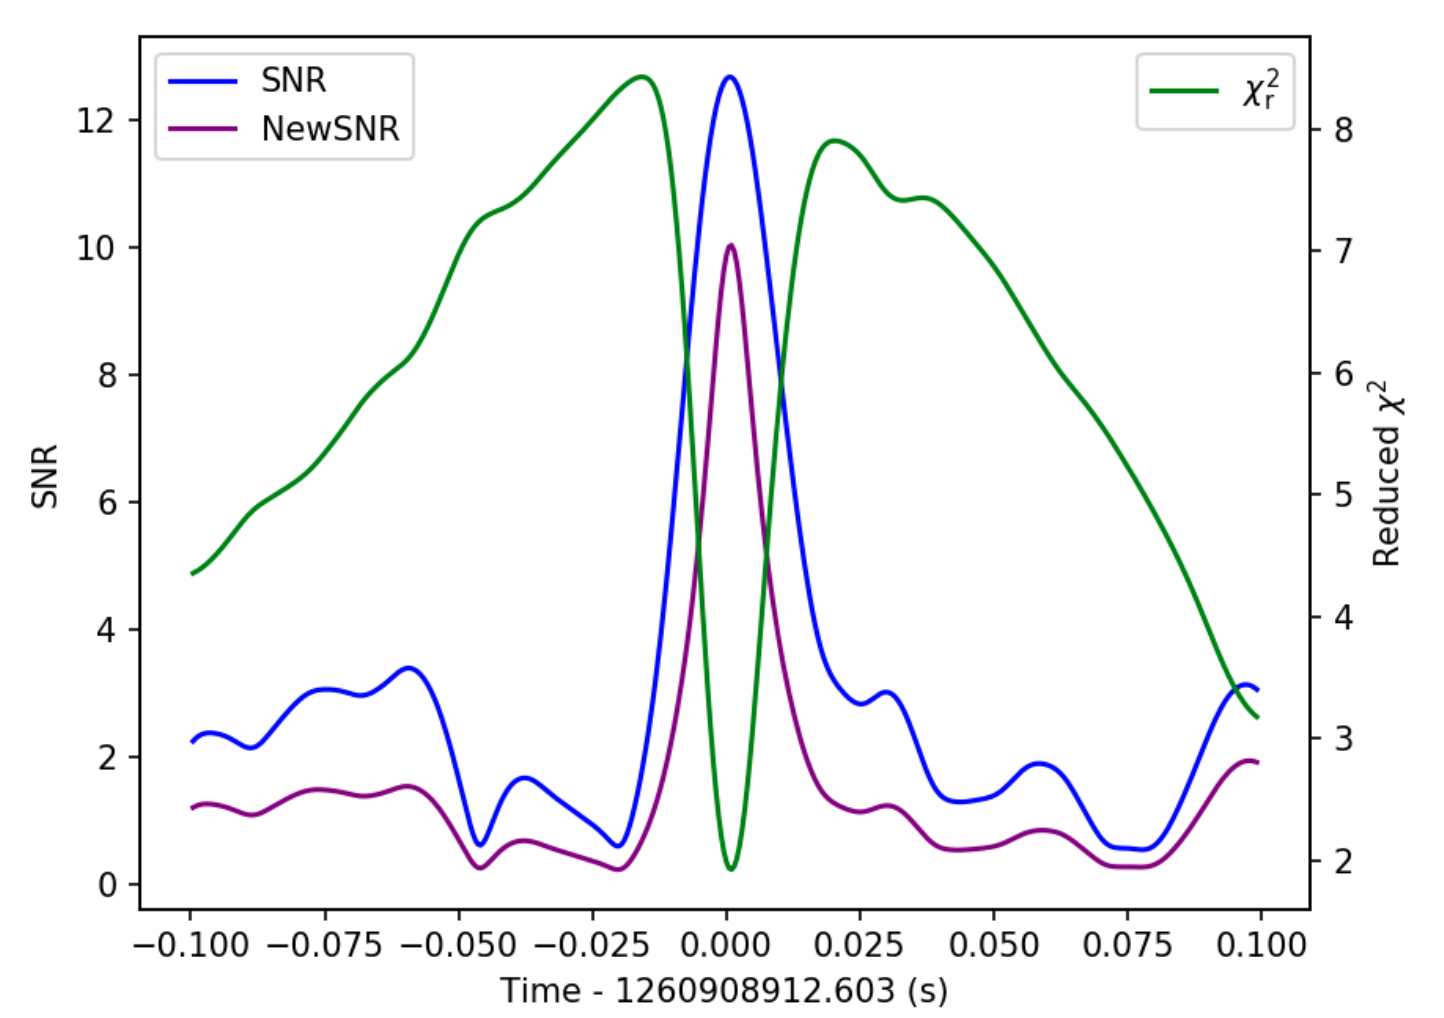
\includegraphics[scale=0.45]{chisquared}}%
          \centering
          \caption{Reduced $\chi^2$-test, SNR, and reweighted SNR
            (``NewSNR'') behaviour at the time of a the blip glitch
            shown in the left panel of Fig.\,\ref{fig:glitches}.  The
            timeseries are reported in green, blue, and purple,
            respectively.}
          \label{fig:chisquared}
        \end{figure}

%L1_Loudest
	The same study is repeated for the loudest single-detector triggers in L1.
	Once more, blip glitches emerged, but also {\it comb-like} glitch packs did (Fig.\,\ref{fig:glitches}, right panel).
        The latter were found to dominate the second bin in the case of L1.
	No other characteristic features were seen in the spectrograms.
	
	A list of the loudest coincident triggers, resulting from the coincident test on the background triggers, 	
	is also available and the follow-up procedure imitates the steps for the loudest single follow-up.
	Events that pass the coincident test are subject to further scrutiny, 
	as these may be affected by glitches or gated data.
        \fpg{Ma del background a 2 detector hai deciso di non parlare?}
        % coincident SNR time series [Eq.\,(\ref{eq:rhocoincPyCBC})].  This operation is repeated with multiple timeshifts to generate the {\it background} trigger distribution, to which the discussion here is limited; the non-timeshifted distribution of triggers constitutes the {\it foreground}, and is not presented in this thesis.

\subsection{Missed Injections}
 The injection campaign consists in generating signals using different waveform models,
        with simulated source parameters generated by random draws from the (multidimensional) prior distribution of physical properties of the sources;
        these sets of simulated GW signals are then injected in the detector data streams.
        Finally, the pipeline runs on such modified (virtual) data streams to recover the injections: this allows one to estimate the search sensitivity and assess its performance.  \fpg{Punta al luogo nella tesi in cui hai discusso queste priors.}

        Figure \ref{fig:inj_plots} summarizes the result of the injection campaigns carried out on the chunk of O3b data.
        Each point in the left panel of Fig.\ref{fig:inj_plots} represents an injection;
        it is placed in the plot according to its chirp mass and optimal SNR,
        a measure of the SNR of the injected waveform assuming no noise is present,
        and it is coloured according to the outcome of its recovery:
        a red cross is an injection that was not recovered,
        while circles are recovered injections coloured by their FAR,
        the dark blue ones being identified undoubtedly as signals, that is,
        they were found to be louder than all background events.

        The right panel in Fig.\ref{fig:inj_plots} shows the distribution of injections and their recovery
        as a function of the injected decisive distance and chirp mass.
        The injected decisive distance is  defined as the injected effective
        distance\footnote{The effective distance of a source is the distance at which an optimally-oriented and located signal would have the produced the same SNR as the given simulation }
        in the second   loudest detector in the detector network.
	Injections with higher chirp mass tend to be found better 
	since they have shorter templates that produce higher SNR triggers. 

        The ability to detect an event depends upon the decisive distance:
        since coincidence is required in at least two detectors for a detection
        if a system has an effective distance small enough to be seen in one detector,
        if the next largest effective distance in another detector is outside the that detector’s range,
        no trigger will be created in that detector, and so no coincident trigger will be generated.

        For all these reasons, the decisive distance along with the chirp mass
        (as the overall amplitude of the GW signal scales with it)
        are the best parameters that encode the expected sensitivity of the search.

         \begin{figure}[t]
          \noindent
          \label{inj_plots}
          \makebox[\textwidth]{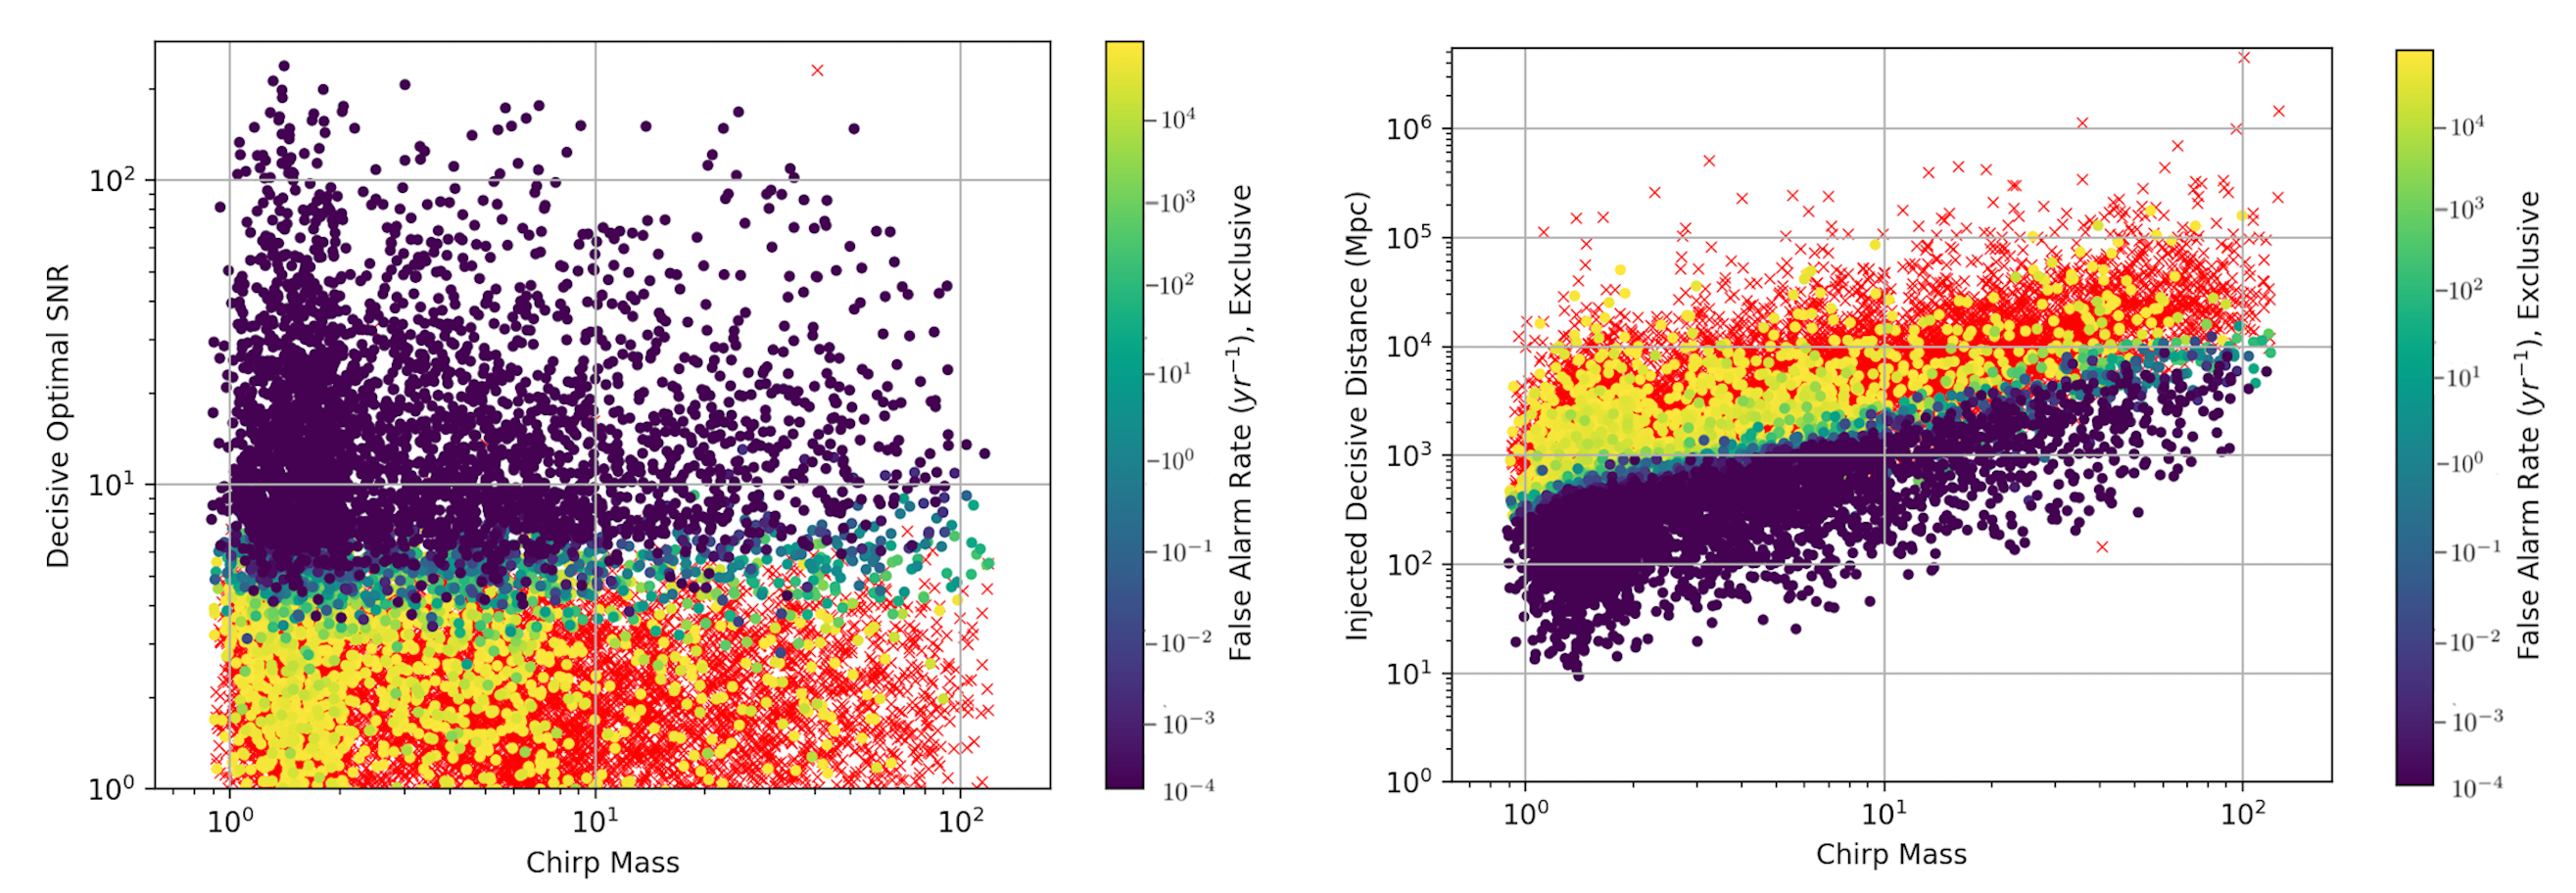
\includegraphics[width=\textwidth]{inj_plots}}%
          \centering
          \caption{{\bf Injection results.} {\textit Left:} Each point represents the source of a simulated GW signal injected in the data and recovered from it.  The horizontal axis reports the chirp mass of the source, while the vertical one is the decisive optimal SNR of the signal, which is the expected SNR in the second most sensitive instrument to that particular source. {\textit Right:} the injected decisive distance  is plotted as a function of the chirp mass.}
          \label{fig:inj_plots}
        \end{figure}

	The loudest missed injections and the poorly recovered ones with optimal SNR greater than 8 are
        examined in detail, in all injection categories.
	Several reasons can cause an injection to be missed or not recovered.
       	\begin{itemize}
          \item Its (optimal) SNR is to weak: this constitutes the bulk of the red crosses in the plot, which represent sources that are too far away to yield a signal that is strong enough to be observed.  Additionally, the search SNR is not necessarily equal to the optimal SNR: the noise realisation around the time of the injection can cause an injection's SNR to drop below the search threshold.
            This is a particularly common cause behind missed BNS injections, as the SNR is accumulated over a wide bandwidth.
          \item A glitch occurred near the injection. For a time much longer than the length of the peak, 
            loud glitches corrupt the SNR and the $\chi^2$ timeseries, which prevents the search from clearly identifying the SNR peak associated with the injection alone.
          \item The injection is near the beginning or the end of a lock period\footnote{Interferometric GW are amplified by several resonant cavities: the interferometer is said to be locked when all of these cavities are held on resonance \cite{108} \fpg{Undefined reference}.}. The high-pass filtering and re-sampling performed by the search alter data at the beginning and end of a segment. Therefore, near a lock transition, the search discards eight seconds of data and injections within or near those eight seconds can be missed.
          \item The physical parameters of the simulated signal fall outside the waveform template parameter range.  Notably, this can happen when an injection represents a strongly precessing system, along the lines of what was discussed for the coherent search.  Since precession significantly modifies the waveform's shape and the template bank only includes waveforms with aligned spins, simulated signals with the spins of the individual objects not aligned with the orbital angular momentum have a non-negligible chance of not being recovered.
          % \item The injection is auto-gated by the search. For example, high-mass injections are very short and easily confused with glitches, leading to be auto-gated by the search.
          \item The injection (partially) overlaps with gated glitches before and just around the time of merger.  An example of this is provided in the spectrogram in Fig.\,\ref{fig:gated_glitch}: the track of the loudest template rung by a BNS injection (blue) is seen to cross two stretches of gated data (green shaded areas), one of which is particularly close to the merger time.
            Gating of data containing glitches is the most frequent cause of missed BBH injections:
            the top panel of Fig.\,\ref{fig:gated} shows the case of an injection with high optimals SNR in both detectors that is not recovered as a coincident trigger because of gated data in L1 around the time of merger.
            Similarly, in the bottom panel the recovery of the injected chirp signal is unsuccessful because of the presence of a loud gated glitch.
        \end{itemize}
    	
        \begin{figure}[t]
          \noindent
          \label{gated_glitch}
          \makebox[\textwidth]{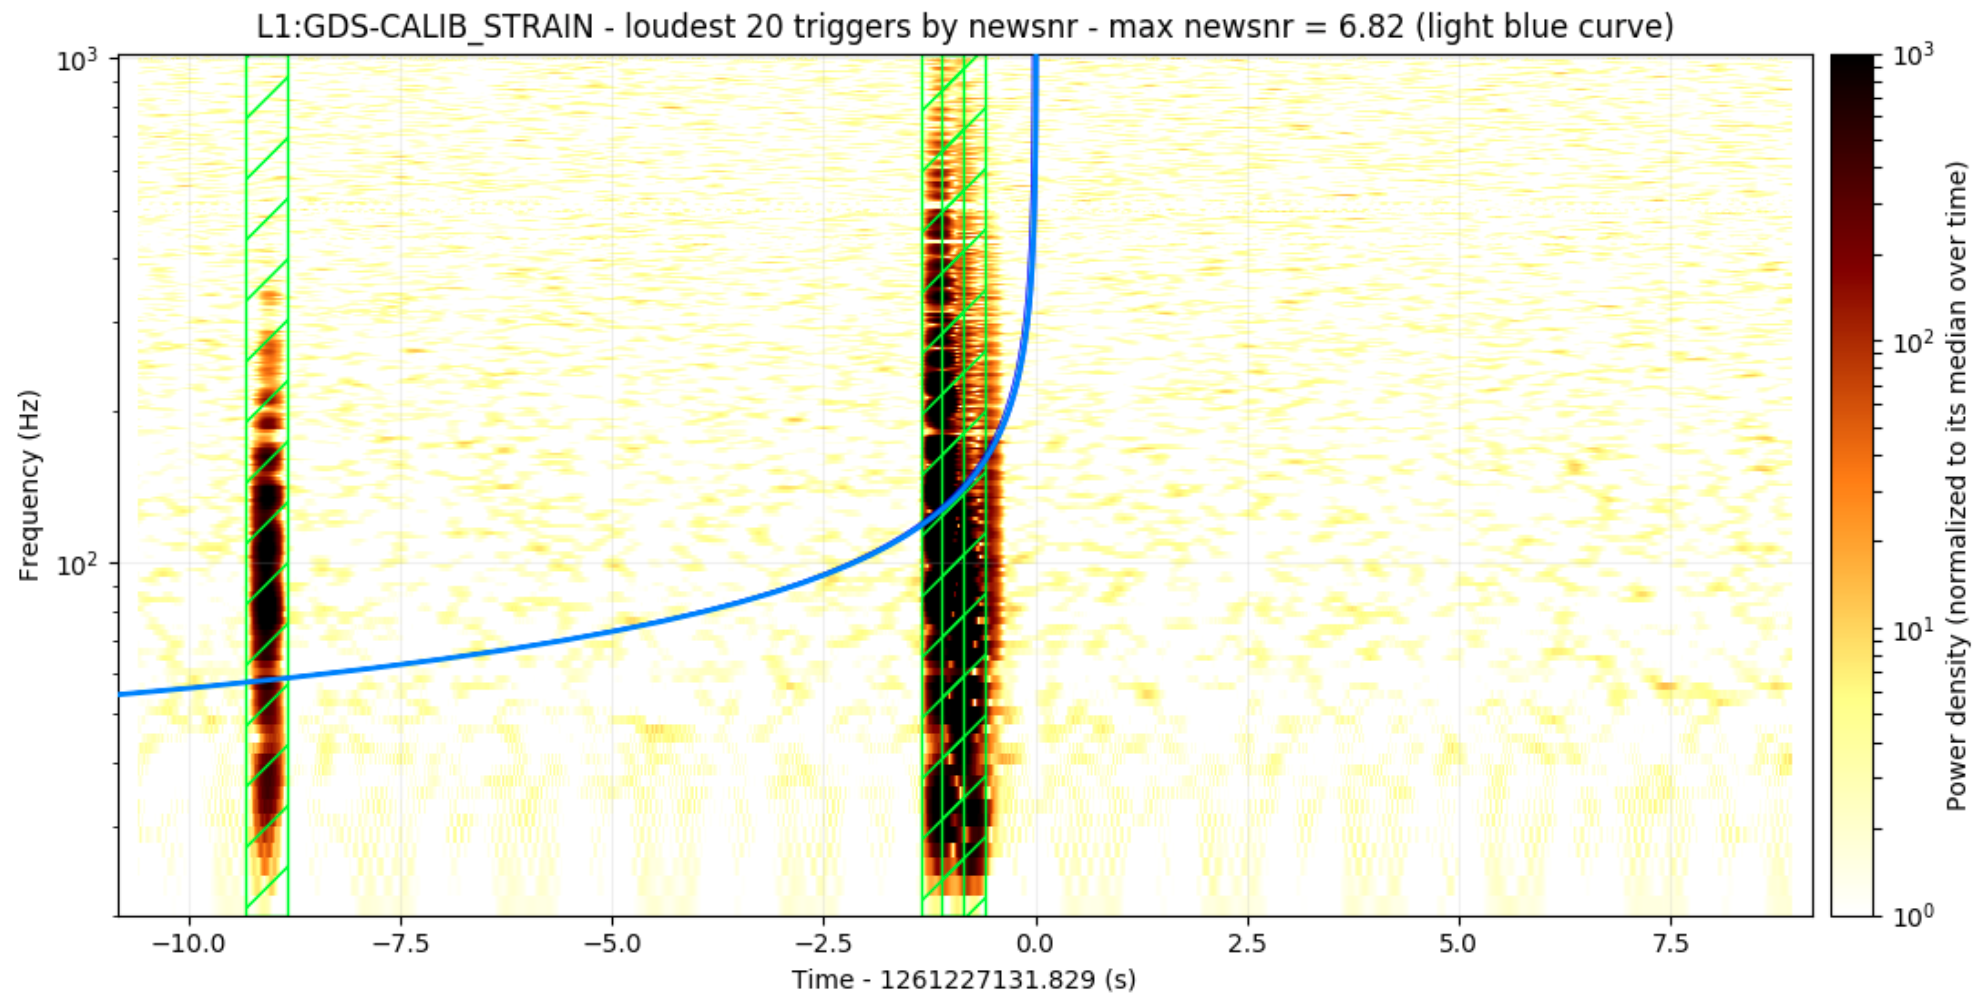
\includegraphics[width=\textwidth]{gated_glitch}}%
          \centering
          \caption{The strain spectrogram for a missed BNS injection: the dark regions represent loud glitches, which are gated by the pipeline (green lines). The ligth blue curve is the loudest template.}
          \label{fig:gated_glitch}
        \end{figure}

        \begin{figure}[t]
          \noindent
          \label{gated}
          \makebox[\textwidth]{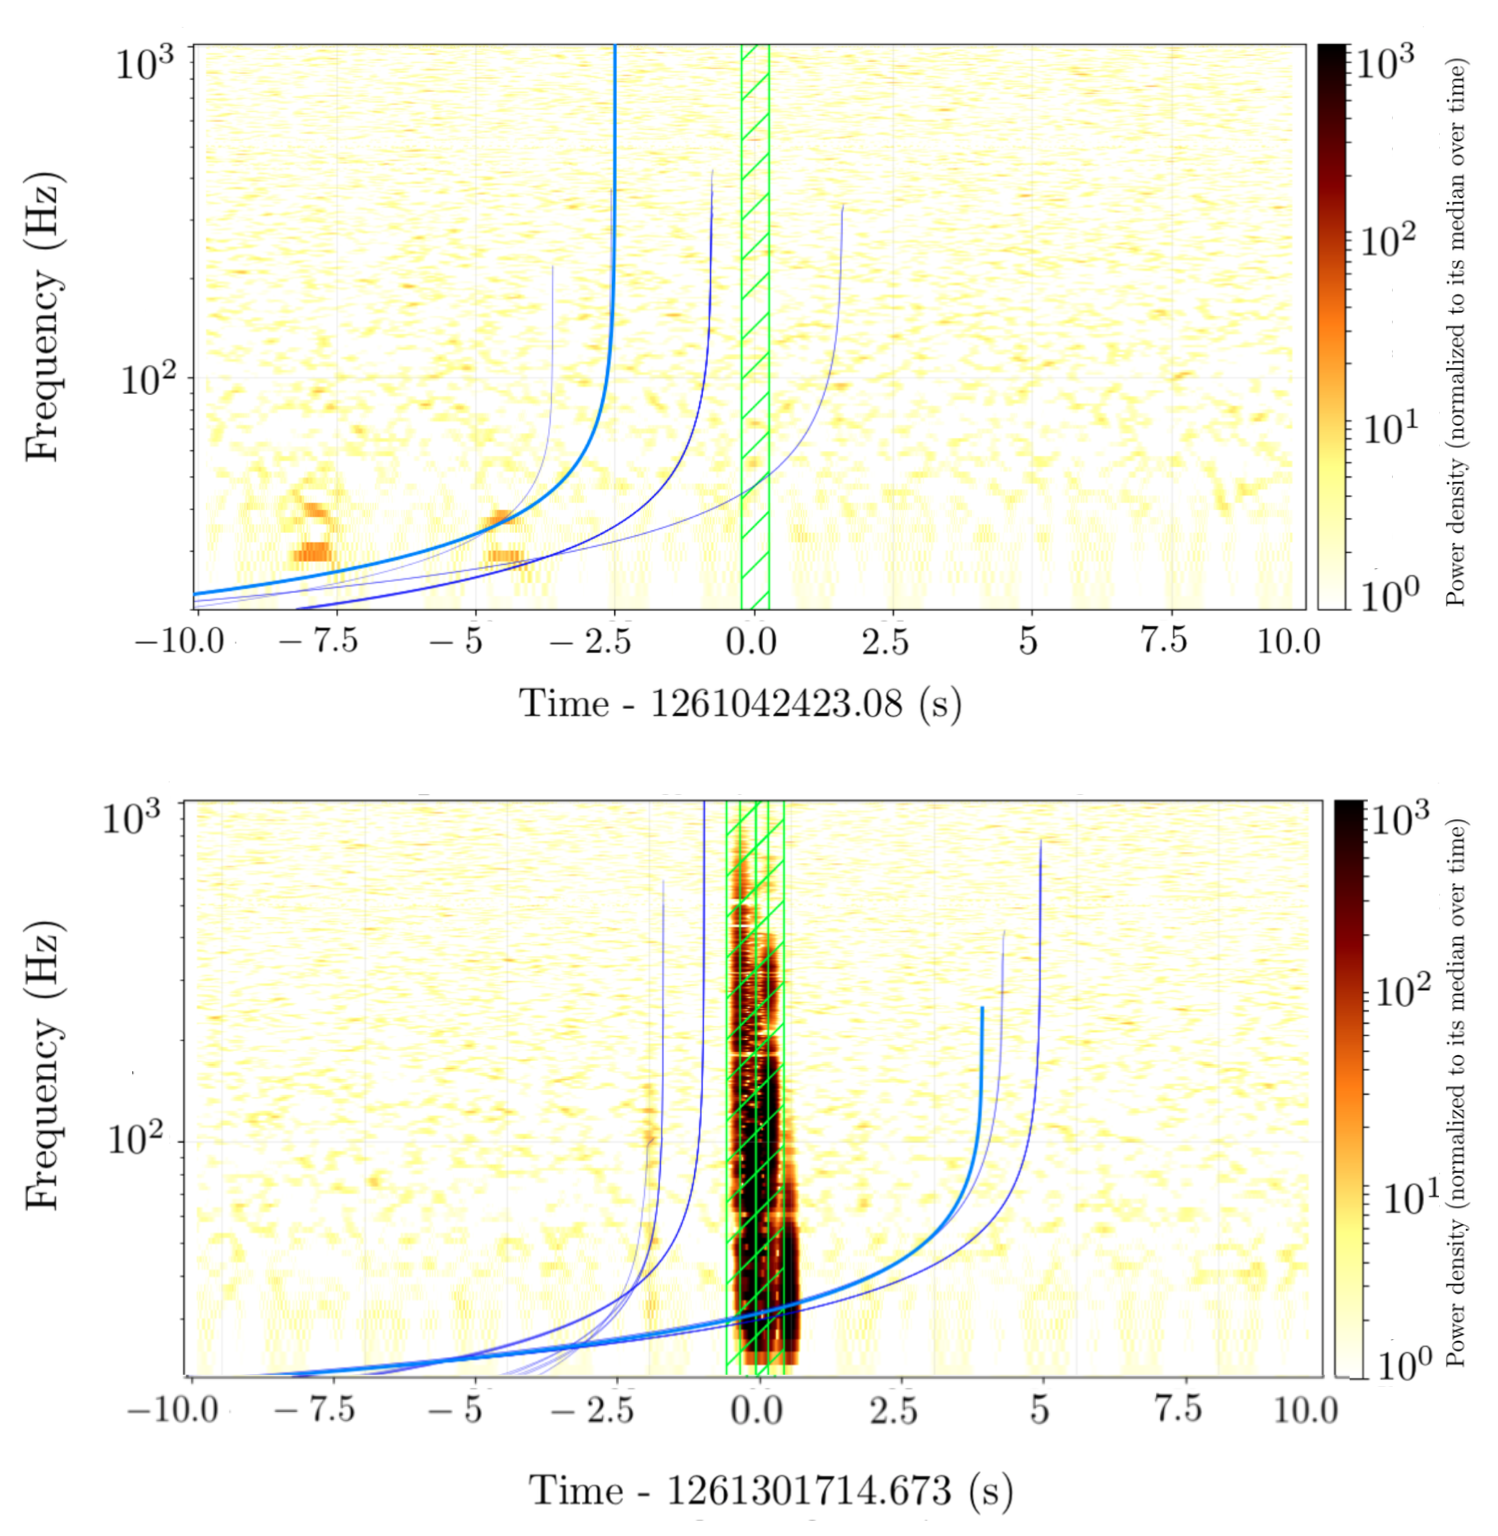
\includegraphics[scale=0.5]{gated}}%
          \centering
          \caption{Spectrogram of two missed BBH injections: the contiuous curves represent the loudest triggers, while gated data is marked by the green mesh.  The top and bottom panels refer to an injection missed due to a gated glitch in L1 data and H1, respectively, that falls nearby the merger time of the injections.  \fpg{Ma perch\'e ci sono varie tracce?}}
          \label{fig:gated}
        \end{figure}

	The follow-up of missed injections with a large SNR is a a useful diagnostic check, 
	as it can be indicative of a noise transient, a gating artefact, or a problem with the analysis configuration itself.
        \fpg{Un paio di frasi su quello che \`e capitato nel tuo chunk.}
	The missed injections in this specific chunk were lost mostly because of very low SNR values.
	However, the loudest missed injection is a BBH simulated signal shown in the top panel of Fig.\,\ref{fig:gated},
	with a decisive optimal SNR of $\sim 230$ and chirp mass of $\sim 40$,
	which also stands out in the left panel of Fig.\,\ref{fig:inj_plots}.
	The background investigations yielded overall good results,
	leading to uncovering of the foreground results:
	these were shared and discussed within the LIGO-Virgo Collaboration, but cannot be discolsed yet.

%--------------------------------------------------------
\chapter*{Conclusions}
\fpg{Giri di correzione: 0.}%
\fpg{Anche qui da quello che vedo il discorso fila poco.  Dividi in capoversi, batti sulla centralit\`a della template bank per fare un intero run, riporta i risultati delle 3 GRB, evidenzia la pubblicazione, ecc.}

	The first measurement of the effect of GWs has opened the gateway to GW astronomy 
	and a new window to the universe, enabling astronomers to look into regions of our cosmos 
	that were inaccessible to regular astronomical observation.
	It has required long years of development, first from a theoretical, 
	then from a technological — especially that of precision laser interferometry— point of view,
	for the detections to become more and more regular recently.
	
	The first direct proof of the existence of BBH was the outcome of years of development, 
	first from a theoretical, then from a technological — especially that of precision laser interferometry— point of view;
	Recently, the detections become more and more regular as the detectors and the data analysis techniques are still improving.
	Search pipelines are algorithms designed to identify GW signals in detector data.
	In this work, I focused explicitly on two offline searches for compact binary coalescences, 
	which are crucial to accurately estimate the significance of the candidate and confidently establish its astrophysical origin.
	describing the different approaches to GW data analysis behind the two searches: coherent and coincident.
	After outlining the theoretical framework of GW astronomy,
        the aforementioned data analysis strategies have been investigated.

	Algorithms requiring coincident detection of a source by multiple detectors,
        are the primary method to detect BBH mergers,
        as shown in the GW event overview in Chapter \ref{ch:ObservingRuns}.
        The benefits of this procedure, described in Sec.\ref{subsec:coincident} are plenty:
        first it immediately eliminates the great majority of noise background
        by rejecting any triggers which are uncorrelated in time in two or more detectors;
        secondly, it is not computationally expensive.
        The dominant cost of the search is in performing the matched filtering (see, Sec.\ref{sec:matched_filtering})
        of the data against the template bank (see, Section \ref{sec:template_banks}).
        The {\ttfamily PyCBC} offline analysis has been developed implementing this method in its algorithms.

        A coherent approach, described in Sec.\ref{subsec:coherent}, on the other hand,
        it is computationally expensive in the case of modelled searches,
        however, knowing the time and sky-location of the source can cut the cost of the search.
        It enables a more extensive search in the GW data, potentially uncovering signals
        that are not within reach to all-sky, all-time searches.
        Moreover, the coherent analysis allows for some additional tests
        which are not readily available in the coincidence case.
        The most significant of these is the null SNR (see, Sec.\ref{subsubsec:nullsnr}) which can be used to reject events which are
        not consistent with two GW polarisations.
        This method is the  basis which the  {\ttfamily PyGRB}  pipeline is built upon (see, Sec.\ref{subsec:pygrb}).

	The two approaches have one main thing in common: the use of a template bank.
	This is the core tool in a matched filtering search,  
	therefore it is crucial that it works efficiently in order to achieve successful detections.
	However, the two pipelines, built upon these two methods, differ in one important aspect: 
	while {\ttfamily PyCBC}  is an all-sky search, {\ttfamily PyGRB} is a targeted one.
	This difference affects the construction of the template bank implemented in the pipeline.
	Since {\ttfamily PyGRB} conducts the analysis only when the CBC signal is associated with an EM transient, GRBs,
	it is sufficient that the template bank covers the parameter space associated with binaries that are EM bright.
	In order to exclude CBC sources that are EM dark from the bank, 
	it is useful to have reliable models of the GW and EM signals powered by EM sources.
	Since one of the likely progenitors of short GRBs are systems that 
	lead to the formation of an accretion torus around the final BH,
	up until O2 included, the EM bright bank employed in the search 
	was generated making use of a remnant mass predictive model.
 	In Sec.\ref{subsubsec:mrem_model} of Chapter \ref{ch:datanalysis} we have compared this model \cite{50}
        with an updated one \cite{54} for the remnant mass of a NSBH system,
	We proceeded to implement this into the EM-bright template bank,
        generated  it within a well defined parameter space and tested it.
        All the results suggest that the template bank is performing exactly as expected,
        covering section of the parameter space which were not well covered before,
        with an average fitting factor for the entire bank of 0.98.
\addcontentsline{toc}{chapter}{Conclusions}
\markboth{Introduction}{Conclusions}

\backmatter
\cleardoublepage

\phantomsection % Give this command only if hyperref is loaded \addcontentsline{toc}{chapter}{\bibname}

\bibliographystyle{plain}
\bibliography{reference}
\end{document} 

